% Options for packages loaded elsewhere
\PassOptionsToPackage{unicode}{hyperref}
\PassOptionsToPackage{hyphens}{url}
\documentclass[11pt]{article}
\usepackage[table]{xcolor}
\usepackage{amsmath,amssymb}

% arXiv-friendly numbering
\setcounter{secnumdepth}{2}
\setcounter{tocdepth}{2}
\usepackage{iftex}
\ifPDFTeX
  \usepackage[T1]{fontenc}
  \usepackage[utf8]{inputenc}
  \usepackage{textcomp} % provide euro and other symbols

  % Minimal Unicode support for text pasted/extracted from DOCX.
  % Keep mappings conservative and math-safe.
  \usepackage{newunicodechar}
  \newunicodechar{′}{\ensuremath{^{\prime}}}
  \newunicodechar{″}{\ensuremath{^{\prime\prime}}}
  \newunicodechar{−}{\ensuremath{-}}
  % Make dashes safe in math mode (prevents "\textendash invalid in math mode" warnings)
  \providecommand{\UnicodeEnDash}{\ifmmode\text{--}\else\textendash\fi}
  \providecommand{\UnicodeEmDash}{\ifmmode\text{---}\else\textemdash\fi}
  \newunicodechar{–}{\UnicodeEnDash}
  \newunicodechar{—}{\UnicodeEmDash}
  \newunicodechar{≤}{\ensuremath{\le}}
  \newunicodechar{≥}{\ensuremath{\ge}}
  \newunicodechar{≈}{\ensuremath{\approx}}
  \newunicodechar{∝}{\ensuremath{\propto}}
  \newunicodechar{∈}{\ensuremath{\in}}
  \newunicodechar{×}{\ensuremath{\times}}
  \newunicodechar{·}{\ensuremath{\cdot}}
  \newunicodechar{∇}{\ensuremath{\nabla}}
  \newunicodechar{∂}{\ensuremath{\partial}}
  \newunicodechar{⊙}{\ensuremath{\odot}}
  \newunicodechar{☉}{\ensuremath{\odot}}
  \newunicodechar{★}{\ensuremath{\star}}
  \newunicodechar{☆}{\ensuremath{\star}}
  \newunicodechar{□}{\ensuremath{\Box}}
  \newunicodechar{■}{\ensuremath{\blacksquare}}
  \newunicodechar{κ}{\ensuremath{\kappa}}
  \newunicodechar{Λ}{\ensuremath{\Lambda}}
  \newunicodechar{Δ}{\ensuremath{\Delta}}
  \newunicodechar{Φ}{\ensuremath{\Phi}}
  \newunicodechar{Ψ}{\ensuremath{\Psi}}
  \newunicodechar{Ω}{\ensuremath{\Omega}}
  \newunicodechar{Υ}{\ensuremath{\Upsilon}}
  \newunicodechar{α}{\ensuremath{\alpha}}
  \newunicodechar{β}{\ensuremath{\beta}}
  \newunicodechar{γ}{\ensuremath{\gamma}}
  \newunicodechar{δ}{\ensuremath{\delta}}
  \newunicodechar{ε}{\ensuremath{\epsilon}}
  \newunicodechar{η}{\ensuremath{\eta}}
  \newunicodechar{λ}{\ensuremath{\lambda}}
  \newunicodechar{μ}{\ensuremath{\mu}}
  \newunicodechar{ν}{\ensuremath{\nu}}
  \newunicodechar{π}{\ensuremath{\pi}}
  \newunicodechar{ρ}{\ensuremath{\rho}}
  \newunicodechar{σ}{\ensuremath{\sigma}}
  \newunicodechar{τ}{\ensuremath{\tau}}
  \newunicodechar{φ}{\ensuremath{\phi}}
  \newunicodechar{χ}{\ensuremath{\chi}}
  \newunicodechar{ψ}{\ensuremath{\psi}}
  \newunicodechar{ω}{\ensuremath{\omega}}
  \newunicodechar{⁻}{\textsuperscript{-}}
  \newunicodechar{⁰}{\textsuperscript{0}}
  \newunicodechar{¹}{\textsuperscript{1}}
  \newunicodechar{²}{\textsuperscript{2}}
  \newunicodechar{³}{\textsuperscript{3}}
  \newunicodechar{⁴}{\textsuperscript{4}}
  \newunicodechar{⁵}{\textsuperscript{5}}
  \newunicodechar{⁶}{\textsuperscript{6}}
  \newunicodechar{⁷}{\textsuperscript{7}}
  \newunicodechar{⁸}{\textsuperscript{8}}
  \newunicodechar{⁹}{\textsuperscript{9}}
\else % if luatex or xetex
  \usepackage{unicode-math} % this also loads fontspec
  \defaultfontfeatures{Scale=MatchLowercase}
  \defaultfontfeatures[\rmfamily]{Ligatures=TeX,Scale=1}
\fi
\usepackage{lmodern}
\ifPDFTeX\else
  % xetex/luatex font selection
\fi
% Use upquote if available, for straight quotes in verbatim environments
\IfFileExists{upquote.sty}{\usepackage{upquote}}{}
\IfFileExists{microtype.sty}{% use microtype if available
  \usepackage[]{microtype}
  \UseMicrotypeSet[protrusion]{basicmath} % disable protrusion for tt fonts
}{}
\makeatletter
\@ifundefined{KOMAClassName}{% if non-KOMA class
  \IfFileExists{parskip.sty}{%
    \usepackage{parskip}
  }{% else
    \setlength{\parindent}{0pt}
    \setlength{\parskip}{6pt plus 2pt minus 1pt}}
}{% if KOMA class
  \KOMAoptions{parskip=half}}
\makeatother
\usepackage{longtable,booktabs,array}
\usepackage{tabularx}
\usepackage{makecell}
\usepackage{pdflscape}
\usepackage[section]{placeins} % provides \FloatBarrier to keep floats within sections

% --- Table styling (professional + readable) ---
\renewcommand{\arraystretch}{1.15} % row height
\setlength{\tabcolsep}{6pt}       % column padding
\definecolor{TableStripe}{gray}{0.94}
\newcommand{\TableHeader}{\bfseries}
\newcommand{\TableHeaderRow}{\rowcolor{black!10}\bfseries}
% Alternating row shading for tables (safe default)
% longtable
\AtBeginEnvironment{longtable}{\rowcolors{2}{TableStripe}{white}}
\AtEndEnvironment{longtable}{\rowcolors{2}{}{}}
% tabular / tabularx
\AtBeginEnvironment{tabular}{\rowcolors{2}{TableStripe}{white}}
\AtEndEnvironment{tabular}{\rowcolors{2}{}{}}
\AtBeginEnvironment{tabularx}{\rowcolors{2}{TableStripe}{white}}
\AtEndEnvironment{tabularx}{\rowcolors{2}{}{}}


% Section divider row for long tables: temporarily disable row striping while inserting the divider
\newcommand{\TableSection}[1]{%
  \hiderowcolors
  \rowcolor{black!15}\multicolumn{5}{@{}l@{}}{\textbf{#1}}\\
  \showrowcolors
}

\newcounter{none} % for unnumbered tables
\usepackage{calc} % for calculating minipage widths
% Correct order of tables after \paragraph or \subparagraph
\usepackage{etoolbox}
\makeatletter
\patchcmd\longtable{\par}{\if@noskipsec\mbox{}\fi\par}{}{}
\makeatother
% Allow footnotes in longtable head/foot
\IfFileExists{footnotehyper.sty}{\usepackage{footnotehyper}}{\usepackage{footnote}}
\makesavenoteenv{longtable}
\usepackage{graphicx}
\makeatletter
\newsavebox\pandoc@box
\newcommand*\pandocbounded[1]{% scales image to fit in text height/width
  \sbox\pandoc@box{#1}%
  \Gscale@div\@tempa{\textheight}{\dimexpr\ht\pandoc@box+\dp\pandoc@box\relax}%
  \Gscale@div\@tempb{\linewidth}{\wd\pandoc@box}%
  \ifdim\@tempb\p@<\@tempa\p@\let\@tempa\@tempb\fi% select the smaller of both
  \ifdim\@tempa\p@<\p@\scalebox{\@tempa}{\usebox\pandoc@box}%
  \else\usebox{\pandoc@box}%
  \fi%
}
% Set default figure placement to htbp
\def\fps@figure{htbp}
\makeatother
\setlength{\emergencystretch}{3em} % prevent overfull lines
\providecommand{\tightlist}{%
  \setlength{\itemsep}{0pt}\setlength{\parskip}{0pt}}
\usepackage{bookmark}
\IfFileExists{xurl.sty}{\usepackage{xurl}}{} % add URL line breaks if available
\urlstyle{same}

% Preprint geometry (clean, arXiv-friendly)
% Slightly tighter than 1in to reduce excessive whitespace.
\usepackage[margin=0.9in]{geometry}

% Citations + BibTeX (arXiv-standard)
% APA 7th author-date citation format (not numbered)
\usepackage[authoryear,round]{natbib}

% Caption styling
\usepackage[font=small,labelfont=bf]{caption}
\captionsetup{compatibility=false}

% Simple header/footer (arXiv-safe)
\usepackage{fancyhdr}
\pagestyle{fancy}
\fancyhf{}
\fancyhead[L]{Intrinsic Response Sector as Dark Gravity}
\fancyhead[R]{Kitcey}
\fancyfoot[C]{\thepage}
\setlength{\headheight}{14pt}

\hypersetup{
  pdftitle={Intrinsic Response Sector as Dark Gravity: A GR-Compatible Candidate Identity for the Cold Dark Matter Role (SPARC-175)},
  hidelinks,
  pdfcreator={LaTeX}}

\title{Intrinsic Response Sector as Dark Gravity:\\
\large A GR-Compatible Candidate Identity for the Cold Dark Matter Role (SPARC-175)}

\author{Robert D.\ Kitcey\\
\normalsize Independent Researcher\\
\normalsize ORCID: 0009-0004-8679-9155\\
\normalsize \texttt{rkitcey@lernaean.net}}

\date{February 2026\\Preprint Draft v5.1}

\begin{document}
\maketitle

\noindent\textbf{Versioned preprint:} Kitcey, R. D. (2026). \emph{Intrinsic Response Sector as Dark Gravity: A GR-Compatible Candidate Identity for the Cold Dark Matter Role (SPARC-175)} (v5.1.0). Zenodo.\,\href{https://doi.org/10.5281/zenodo.18778895}{doi:10.5281/zenodo.18778895}

\begin{abstract}
We present a falsification-first, galaxy-domain framework for explaining rotation-curve anomalies without assuming particulate cold dark matter. Working within standard general relativity (GR), we define a response-sector stress--energy \(T_{\mu\nu}^{\mathrm{resp}}\) as the minimal effective source required so that the weak-field metric potentials inferred from kinematics satisfy the Einstein equation with baryons. This definition is ontologically agnostic and is best read as an effective field theory/constitutive-closure candidate. Observed rotation curves define a model-independent residual, which we compress with a one-parameter boundary-layer closure activated near a baryonic transition radius \(R_{t}\) and constrained by an approximate flux-conservation law outside the activation zone.

Applied to 175 galaxies from the SPARC database, this model yields very strong improvement over a baryons-only model for 92\% of systems and passes a Bayesian Information Criterion (BIC) overfitting test in 97\% of cases. Crucially, we demonstrate that this 1-parameter response model is strongly preferred by BIC over standard 2-parameter NFW and Burkert dark matter halo models in over 90\% of the SPARC sample. Further, 5-fold cross-validation shows the response model has significantly lower out-of-sample prediction error (mean RMSE = 3.1 km/s) than the NFW model (mean RMSE = 4.9 km/s). A cymatics-inspired extension explores oscillatory signatures in residuals as eigenmodes of a linearized response operator, providing a spectral taxonomy for response morphologies and predicting higher-harmonic content in galaxies with sharp baryonic gradients (Appendix D) \citep{Rossing1982Chladni, Tuan2014Nodal, BenderOrszag1999}. The baryonic Tully--Fisher relation is recovered as an empirical consequence (Spearman \(r_{s} = 0.95\)). These results establish the response sector as a parsimonious and predictively powerful alternative to standard halo models for describing galactic dynamics.
\end{abstract}

\noindent\textbf{Keywords:} galaxy rotation curves, dark matter alternatives, dark matter candidates, dark matter identity, general relativity, gravitation, effective field theory, response-sector stress--energy, boundary-layer physics, SPARC database, falsification criteria, Bayesian model comparison, cross-validation

\section*{Executive Summary}
\addcontentsline{toc}{section}{Executive Summary}

The dark-matter paradigm explains galactic rotation curve anomalies by postulating a new, non-luminous matter component. Despite decades of null results in direct, indirect, and collider searches, the hypothesis persists largely because no comparably rigorous alternative has been tested against the full breadth of observational data. This paper develops and tests such an alternative. We keep the Einstein tensor standard (general relativity) and do not assume particulate cold dark matter (CDM). Instead, we use observed galactic phenomenology---rotation curves from the SPARC database of 175 galaxies---to infer the effective potentials and effective stress--energy required on the right-hand side of the Einstein equation, then compress that freedom with a low-degree-of-freedom ``intrinsic medium response'' closure.

The organizing principle is \(G_{\mu\nu} = 8\pi G\left( T_{\mu\nu}^{\text{bar}} + T_{\mu\nu}^{\text{resp}} \right)\), where \(T_{\mu\nu}^{\text{resp}}\) is the response-sector stress--energy that

\begin{enumerate}
\def\labelenumi{(\roman{enumi})}
\item
  explains galaxy halo phenomenology without particulate CDM, and
\item
  admits a cosmological completion consistent with the empirical ΛCDM success set.
\end{enumerate}

The response sector is activated near a baryonic boundary layer, produces an asymptotic \(\frac{1}{R}\) tail in the extra acceleration, and is described by ≤2 degrees of freedom per galaxy. Across 175 SPARC galaxies, 92\% show very strong improvement over baryons-only, 97\% pass BIC overfitting tests, and the baryonic Tully--Fisher relation emerges as a consequence rather than an imposed prior.

We present explicit falsification criteria, discriminant tests (including lensing-facing statements and cosmological viability requirements), and a domain-partitioned roadmap from galaxy phenomenology through gravitational slip to large-scale structure. Claims are partitioned by domain: this work establishes the galaxy-domain closure and enumerates the cosmological completion requirements and discriminants.

\clearpage
\tableofcontents
\listoftables
\listoffigures
\clearpage
\iffalse % legacy Pandoc-generated TOC/list (disabled)
\hyperref[abstract]{Abstract \hyperref[abstract]{1}}

\hyperref[table-of-contents]{Table of Contents \hyperref[table-of-contents]{4}}

\hyperref[tables]{Tables \hyperref[tables]{7}}

\hyperref[table-of-figures]{Table of Figures \hyperref[table-of-figures]{7}}

\hyperref[introduction]{1. Introduction \hyperref[introduction]{8}}

\hyperref[from-phenomenology-to-effective-source-the-inverse-gr-construction]{2. From Phenomenology to Effective Source: The Inverse-GR Construction \hyperref[from-phenomenology-to-effective-source-the-inverse-gr-construction]{10}}

\hyperref[kinematics-to-required-radial-acceleration]{2.1 Kinematics to Required Radial Acceleration \hyperref[kinematics-to-required-radial-acceleration]{10}}

\hyperref[weak-field-metric-potentials]{2.2 Weak-Field Metric Potentials \hyperref[weak-field-metric-potentials]{10}}

\hyperref[effective-enclosed-mass-and-density]{2.3 Effective Enclosed Mass and Density \hyperref[effective-enclosed-mass-and-density]{10}}

\hyperref[effective-stressenergy-what-is-being-added-in-gr]{2.4 Effective Stress--Energy: What Is Being Added in GR \hyperref[effective-stress-energy-what-is-being-added-in-gr]{11}}

\hyperref[conservation-constraint]{2.5 Conservation Constraint \hyperref[conservation-constraint]{11}}

\hyperref[minimal-response-sector-model-specification]{3. Minimal Response-Sector Model Specification \hyperref[minimal-response-sector-model-specification]{12}}

\hyperref[design-principles]{3.1 Design Principles \hyperref[design-principles]{12}}

\hyperref[auxiliary-field-boundary-layer-model]{3.2 Auxiliary-Field Boundary-Layer Model \hyperref[auxiliary-field-boundary-layer-model]{12}}

\hyperref[operational-implementation]{3.3 Operational Implementation \hyperref[operational-implementation]{12}}

\hyperref[the-constitutive-gravitational-dielectric-alternative]{3.4 The Constitutive ``Gravitational Dielectric'' Alternative \hyperref[the-constitutive-gravitational-dielectric-alternative]{13}}

\hyperref[three-completion-routes]{3.5 Three Completion Routes \hyperref[three-completion-routes]{13}}

\hyperref[data-and-pipeline]{4. Data and Pipeline \hyperref[data-and-pipeline]{14}}

\hyperref[the-sparc-database]{4.1 The SPARC Database \hyperref[the-sparc-database]{14}}

\hyperref[baryonic-velocity-construction]{4.2 Baryonic Velocity Construction \hyperref[baryonic-velocity-construction]{14}}

\hyperref[transition-radius-determination]{4.3 Transition Radius Determination \hyperref[transition-radius-determination]{14}}

\hyperref[fit-procedure-and-amplitude-determination]{4.4 Fit Procedure and Amplitude Determination \hyperref[fit-procedure-and-amplitude-determination]{14}}

\hyperref[six-panel-diagnostic-atlas]{4.5 Six-Panel Diagnostic Atlas \hyperref[six-panel-diagnostic-atlas]{15}}

\hyperref[results-across-175-sparc-galaxies]{5. Results Across 175 SPARC Galaxies \hyperref[results-across-175-sparc-galaxies]{16}}

\hyperref[model-selection-via-bayesian-information-criterion]{5.1 Model Selection via Bayesian Information Criterion \hyperref[model-selection-via-bayesian-information-criterion]{16}}

\hyperref[out-of-sample-predictive-performance]{5.2 Out-of-Sample Predictive Performance \hyperref[out-of-sample-predictive-performance]{17}}

\hyperref[global-fit-performance]{5.3 Global Fit Performance \hyperref[global-fit-performance]{18}}

\hyperref[representative-galaxy-diagnostics]{5.4 Representative Galaxy Diagnostics \hyperref[representative-galaxy-diagnostics]{19}}

\hyperref[emergent-baryonic-tullyfisher-relation]{5.5 Emergent Baryonic Tully--Fisher Relation \hyperref[emergent-baryonic-tullyfisher-relation]{22}}

\hyperref[fitted-vs.-robust-amplitude-comparison]{5.6 Fitted vs. Robust Amplitude Comparison \hyperref[fitted-vs.-robust-amplitude-comparison]{22}}

\hyperref[mass-to-light-ratio-sensitivity]{5.7 Mass-to-Light Ratio Sensitivity \hyperref[mass-to-light-ratio-sensitivity]{23}}

\hyperref[oscillatory-signatures-and-negative-q-galaxies]{5.8 Oscillatory Signatures and Negative-Q Galaxies \hyperref[oscillatory-signatures-and-negative-q-galaxies]{23}}

\hyperref[empirical-validation-ladder]{6. Empirical Validation Ladder \hyperref[empirical-validation-ladder]{22}}

\hyperref[step-1-data-reproducibility]{6.1 Step 1: Data Reproducibility \hyperref[step-1-data-reproducibility]{22}}

\hyperref[step-2-baseline-fits-and-residual-definitions]{6.2 Step 2: Baseline Fits and Residual Definitions \hyperref[step-2-baseline-fits-and-residual-definitions]{22}}

\hyperref[step-3-non-fragile-inference]{6.3 Step 3: Non-Fragile Inference \hyperref[step-3-non-fragile-inference]{22}}

\hyperref[step-4-stratified-permutation-stress-tests]{6.4 Step 4: Stratified Permutation Stress Tests \hyperref[step-4-stratified-permutation-stress-tests]{22}}

\hyperref[step-5-out-of-sample-cross-validation]{6.5 Step 5: Out-of-Sample Cross-Validation \hyperref[step-5-out-of-sample-cross-validation]{22}}

\hyperref[step-6-negative-controls]{6.6 Step 6: Negative Controls \hyperref[step-6-negative-controls]{23}}

\hyperref[falsification-criteria-and-discriminant-tests]{7. Falsification Criteria and Discriminant Tests \hyperref[falsification-criteria-and-discriminant-tests]{24}}

\hyperref[criterion-1-compression-failure]{7.1 Criterion 1: Compression Failure \hyperref[criterion-1-compression-failure]{24}}

\hyperref[criterion-2-out-of-sample-prediction-failure]{7.2 Criterion 2: Out-of-Sample Prediction Failure \hyperref[criterion-2-out-of-sample-prediction-failure]{24}}

\hyperref[criterion-3-gravitational-slip-lensing-inconsistency]{7.3 Criterion 3: Gravitational Slip / Lensing Inconsistency \hyperref[criterion-3-gravitational-slip-lensing-inconsistency]{24}}

\hyperref[criterion-4-cosmological-growth-incompatibility]{7.4 Criterion 4: Cosmological Growth Incompatibility \hyperref[criterion-4-cosmological-growth-incompatibility]{24}}

\hyperref[the-discriminant-triad]{7.5 The Discriminant Triad \hyperref[the-discriminant-triad]{25}}

\hyperref[lensing-and-cosmological-viability]{8. Lensing and Cosmological Viability \hyperref[lensing-and-cosmological-viability]{26}}

\hyperref[lensing-the-weyl-potential-constraint]{8.1 Lensing: The Weyl Potential Constraint \hyperref[lensing-the-weyl-potential-constraint]{26}}

\hyperref[working-hypothesis-metric-equivalence]{8.1.1 Working Hypothesis: Metric Equivalence \hyperref[working-hypothesis-metric-equivalence]{26}}

\hyperref[gravitational-slip-as-a-discriminant]{8.1.2 Gravitational Slip as a Discriminant \hyperref[gravitational-slip-as-a-discriminant]{26}}

\hyperref[cosmological-background]{8.2 Cosmological Background \hyperref[cosmological-background]{26}}

\hyperref[cosmological-perturbations]{8.3 Cosmological Perturbations \hyperref[cosmological-perturbations]{27}}

\hyperref[domain-partition-and-honest-scope]{8.4 Domain Partition and Honest Scope \hyperref[domain-partition-and-honest-scope]{27}}

\hyperref[discussion]{9. Discussion \hyperref[discussion]{28}}

\hyperref[the-response-sector]{9.1 The Response Sector \hyperref[the-response-sector]{28}}

\hyperref[relation-to-mond-and-teves]{9.2 Relation to MOND and TeVeS \hyperref[relation-to-mond-and-teves]{28}}

\hyperref[relation-to-emergent-gravity-and-nonlocal-gravity]{9.3 Relation to Emergent Gravity and Nonlocal Gravity \hyperref[relation-to-emergent-gravity-and-nonlocal-gravity]{28}}

\hyperref[strengths-of-the-current-work]{9.4 Strengths of the Current Work \hyperref[strengths-of-the-current-work]{28}}

\hyperref[limitations-and-open-questions]{9.5 Limitations and Open Questions \hyperref[limitations-and-open-questions]{29}}

\hyperref[the-historical-lesson]{9.6 The Historical Lesson \hyperref[the-historical-lesson]{29}}

\hyperref[a-candidate-identity-for-the-cold-dark-matter-role]{9.7 A Candidate Identity for the Cold Dark Matter Role \hyperref[a-candidate-identity-for-the-cold-dark-matter-role]{29}}

\hyperref[role-vs.-identity-a-formal-distinction]{9.7.1 Role vs. Identity: A Formal Distinction \hyperref[role-vs.-identity-a-formal-distinction]{29}}

\hyperref[defining-the-cdm-role]{9.8. Defining the CDM Role \hyperref[defining-the-cdm-role]{29}}

\hyperref[the-intrinsic-response-as-a-candidate-identity]{9.9. The Intrinsic Response as a Candidate Identity \hyperref[the-intrinsic-response-as-a-candidate-identity]{30}}

\hyperref[a-falsifiable-validation-plan-the-discriminants-ladder]{9.9.1. A Falsifiable Validation Plan: The Discriminants Ladder \hyperref[a-falsifiable-validation-plan-the-discriminants-ladder]{30}}

\hyperref[development-gateway-branch-selection-as-an-explicit-research-fork]{9.9.2 Development Gateway: Branch Selection as an Explicit Research Fork \hyperref[development-gateway-branch-selection-as-an-explicit-research-fork]{30}}

\hyperref[from-critique-to-collaboration-a-playbook-for-scientific-engagement]{9.9.3 From Critique to Collaboration: A Playbook for Scientific Engagement \hyperref[from-critique-to-collaboration-a-playbook-for-scientific-engagement]{33}}

\hyperref[conclusion-the-case-for-engagement]{9.9.4 Conclusion: The Case for Engagement \hyperref[conclusion-the-case-for-engagement]{33}}

\hyperref[discussion-references]{Discussion References \hyperref[discussion-references]{34}}

\hyperref[conclusion]{10. Conclusion \hyperref[conclusion]{35}}

\hyperref[the-framework-stands-or-falls-on-these-empirical-discriminants.-if-it-survives-them-without-reintroducing-an-independent-freely-specified-pressureless-dark-fluid-intrinsic-response-remains-a-viable-candidate-identity-for-the-cdm-role-if-not-it-is-falsified.]{The framework stands or falls on these empirical discriminants. If it survives them without reintroducing an independent, freely specified pressureless dark fluid, intrinsic response remains a viable candidate identity for the CDM role; if not, it is falsified. \hyperref[the-framework-stands-or-falls-on-these-empirical-discriminants.-if-it-survives-them-without-reintroducing-an-independent-freely-specified-pressureless-dark-fluid-intrinsic-response-remains-a-viable-candidate-identity-for-the-cdm-role-if-not-it-is-falsified.]{35}}

\hyperref[appendix-a-comprehensive-symbol-glossary]{Appendix A: Comprehensive Symbol Glossary+ \hyperref[appendix-a-comprehensive-symbol-glossary]{36}}

\hyperref[appendix-b-per-galaxy-mathbfq_mathbfest-mathbfq_mathbfbest-summary-175-galaxies]{Appendix B: Per-Galaxy \(\mathbf{Qest}\) / \(\mathbf{Qbest}\) Summary (175 galaxies) \hyperref[appendix-b-per-galaxy-mathbfq_mathbfest-mathbfq_mathbfbest-summary-175-galaxies]{48}}

\hyperref[appendix-c.-cluster-morphology-operator-and-hff-benchmark]{Appendix C. Cluster morphology operator and HFF benchmark \hyperref[appendix-c.-cluster-morphology-operator-and-hff-benchmark]{58}}

\hyperref[c.1-data-provenance-and-scope]{C.1 Data provenance and scope \hyperref[c.1-data-provenance-and-scope]{58}}

\hyperref[c.2-preregistered-morphology-operator]{C.2 Preregistered morphology operator \hyperref[c.2-preregistered-morphology-operator]{58}}

\hyperref[c.3-robustness-grid-multi-team-systematics-and-roi-sensitivity]{C.3 Robustness grid: multi-team systematics and ROI sensitivity \hyperref[c.3-robustness-grid-multi-team-systematics-and-roi-sensitivity]{59}}

\hyperref[c.4-six-panel-diagnostic-figures-roi-100]{C.4 Six-panel diagnostic figures (ROI = 100″) \hyperref[c.4-six-panel-diagnostic-figures-roi-100]{59}}

\hyperref[appendix-d.-spectral-harmonics-and-the-cymatic-analogy-in-intrinsic-response-theory]{Appendix D. Spectral Harmonics and the Cymatic Analogy in Intrinsic Response Theory \hyperref[appendix-d.-spectral-harmonics-and-the-cymatic-analogy-in-intrinsic-response-theory]{62}}

\hyperref[d.1-purpose-and-scope]{D.1 Purpose and scope \hyperref[d.1-purpose-and-scope]{62}}

\hyperref[d.2-unified-operator-statement-dna-of-intrinsic-response]{D.2 Unified operator statement (``DNA'' of intrinsic response) \hyperref[d.2-unified-operator-statement-dna-of-intrinsic-response]{62}}

\hyperref[d.3-where-harmonics-live-in-a-unified-spacetime-theory]{D.3 Where ``harmonics'' live in a unified spacetime theory \hyperref[d.3-where-harmonics-live-in-a-unified-spacetime-theory]{62}}

\hyperref[d.4-observable-proxy-node-count-and-ux3b4-sign-flips-in-the-sparc-window]{D.4 Observable proxy: node count and Δ-sign flips in the SPARC window \hyperref[d.4-observable-proxy-node-count-and-ux3b4-sign-flips-in-the-sparc-window]{63}}

\hyperref[d.5-consequences-for-lensing-and-stability-constraints]{D.5 Consequences for lensing and stability constraints \hyperref[d.5-consequences-for-lensing-and-stability-constraints]{63}}

\hyperref[references]{References \hyperref[references]{64}}

\section{Tables}\label{tables}

\hyperref[_Toc222952631]{Table 1. Global fit performance of the single-parameter boundary-layer response model across 175 SPARC galaxies. \hyperref[_Toc222952631]{16}}

\hyperref[_Toc222952632]{Table 2. Rung Table (Branch A) \hyperref[_Toc222952632]{31}}

\hyperref[_Toc222952633]{Table 3. Rung Table (Branch B) \hyperref[_Toc222952633]{32}}

\hyperref[_Toc222952634]{Table 4. Criticism and Rebuttal. \hyperref[_Toc222952634]{33}}

\hyperref[_Toc222952635]{Table 5. Comprehensive Symbol Glossary \hyperref[_Toc222952635]{36}}

\hyperref[_Toc222952636]{Table 6. Per-Galaxy \(Qest\) / \(Qbest\) Summary (175 galaxies) \hyperref[_Toc222952636]{48}}

\section{Table of Figures}\label{table-of-figures}

\hyperref[_Toc222952637]{Figure 1. Conceptual schematic of the response-sector framework. \hyperref[_Toc222952637]{9}}

\hyperref[fig:bic_cv_1]{Figure 1a. Bayesian Model Comparison and Cross-Validation Performance (6-panel). \hyperref[fig:bic_cv_1]{16}}

\hyperref[_Toc222952638]{Figure 2. NGC 2403---a well-resolved, intermediate-mass spiral. \hyperref[_Toc222952638]{19}}

\hyperref[_Toc222952639]{Figure 3. DDO 154---a gas-dominated dwarf irregular galaxy. \hyperref[_Toc222952639]{18}}

\hyperref[_Toc222952640]{Figure 4. NGC 2841---a massive, high-surface-brightness spiral. \hyperref[_Toc222952640]{19}}

\hyperref[_Toc222952641]{Figure 5. UGC 06614---a low-surface-brightness galaxy. \hyperref[_Toc222952641]{20}}

\hyperref[_Toc222952642]{Figure 6. HFF \(\kappa\)--X-ray systematics summary at ROI = 100″. \hyperref[_Toc222952642]{59}}

\hyperref[_Toc222952643]{Figure 7. Abell 2744 (CATS v4.1), ROI = 100″ \hyperref[_Toc222952643]{60}}

\hyperref[_Toc222952644]{Figure 8. MACS J0416.1−2403 (CATS v4.1), ROI = 100″. \hyperref[_Toc222952644]{61}}

\fi

\section{Introduction}\label{introduction}

For nearly a century, gravitational anomalies at galactic and cosmological scales have been parameterized by an additional non-luminous sector. The concept originated with Zwicky's observations of the Coma cluster \citep{Zwicky1933Coma}, and anomalies in classical orbital mechanics---such as Mercury's perihelion precession historically attributed to the unseen planet Vulcan \citep{LeVerrier1859Mercury}---have precedent in gravitational physics. The ΛCDM concordance model fits the CMB, BAO, and large-scale structure \citep{Riess2019LMC, Ivezic2019LSST, Euclid2022WideSurvey, Euclid2025Overview} with high precision when cold dark matter (CDM) is treated as an effectively pressureless gravitating component.

Yet the microphysical identity of that dominant non-baryonic component remains empirically unresolved. Many canonical weak-scale interaction scenarios have been constrained by direct detection, indirect searches, and collider experiments. Leading direct-detection experiments including \citep{Akerib2017LUX, Aprile2018XENON1T, Cui2017PandaX} have placed increasingly stringent bounds on traditional WIMP parameter spaces. Indirect searches \citep{Aguilar2013AMS} have further restricted viable dark-matter models. This motivates renewed attention to alternatives that treat the dark sector first as an empirical \emph{role} and only secondarily as an ontological \emph{identity}.

This paper develops an inverse-GR alternative consistent with the Discussion framing in §9: we retain standard GR \citep{Einstein1916GR, Wald1984GR} on the left-hand side and ask what effective stress--energy must appear on the right-hand side if we do not assume particulate CDM. The organizing equation is
\begin{equation}
G_{\mu\nu} = 8\pi G\,\left( T_{\mu\nu}^{\text{bar}} + T_{\mu\nu}^{\text{resp}} \right)
\label{eq:einstein-field-response}
\end{equation}
where \(T_{\mu\nu}^{\text{resp}}\) is defined as the effective response sector required by the observed phenomenology. We demonstrate that a simple, one-parameter closure for \(T_{\mu\nu}^{\text{resp}}\) not only explains galactic rotation curves but does so with \textbf{higher statistical preference} (lower Bayesian Information Criterion) and \textbf{greater predictive accuracy} (lower out-of-sample error via cross-validation) than standard two-parameter dark matter halo models---a claim supported by rigorous comparison across 175 SPARC galaxies (\S5). This definition remains ontologically agnostic; we do not claim spacetime is literally a fluid or solid, only that it admits an EFT/constitutive response closure \citep{Carroll2004Spacetime, Carroll2019Spacetime}.

In the circular-orbit regime, the data provide \(V_{\text{obs}}(R)\) and therefore \(g_{\text{obs}}(R) = V_{\text{obs}}^{2}(R)\text{/}R\). The baryonic prediction \(V_{\text{bar}}(R)\) is assembled from SPARC's stellar and gas components with specified mass-to-light ratios. The model-independent residual \(\Delta(R) \equiv V_{\text{obs}}^{2}(R) - V_{\text{bar}}^{2}(R)\) defines the ``missing curvature'' attributable in ΛCDM to a halo, and attributable here to the response sector.

The inverse mapping alone is underdetermined: many effective sources could reproduce a given \(\Delta(R)\). The scientific content of this work is therefore \textbf{compression}. We impose a boundary-layer closure in which the response activates near a baryonic transition radius \(R_{t}\) (operationally where \(g_{\text{bar}}\left( R_{t} \right) \approx a_{0}\)) and satisfies an approximate flux-conservation law outside the activation zone, yielding an asymptotic \(g_{\text{extra}} \propto 1\text{/}R\) tail with ≤2 degrees of freedom per galaxy.

We further distinguish \(Q_{\text{best}}\) (a global fit amplitude under the imposed closure) from \(Q_{\text{est}}\) (a robust outer estimator computed directly from the outer \(\Delta(R)\) subset). Their strong agreement in rank across SPARC-175 supports the interpretation that the inferred response amplitude tracks genuine outer physics, while deviations diagnose where a single fixed shape requires extension.

Rotation curves primarily constrain the Newtonian-gauge potential \(\Phi\); lensing constrains the Weyl potential \(\Phi_{W} \equiv (\Phi + \Psi)\text{/}2\). Consistent with §9, we treat lensing as a gateway discriminant between Branch A (metric equivalence, \(\Phi \simeq \Psi\)) and Branch B (slip-allowed, \(\eta \equiv \Psi\text{/}\Phi \neq 1\) localized to activation zones).

\begin{figure}[!htbp]
\centering
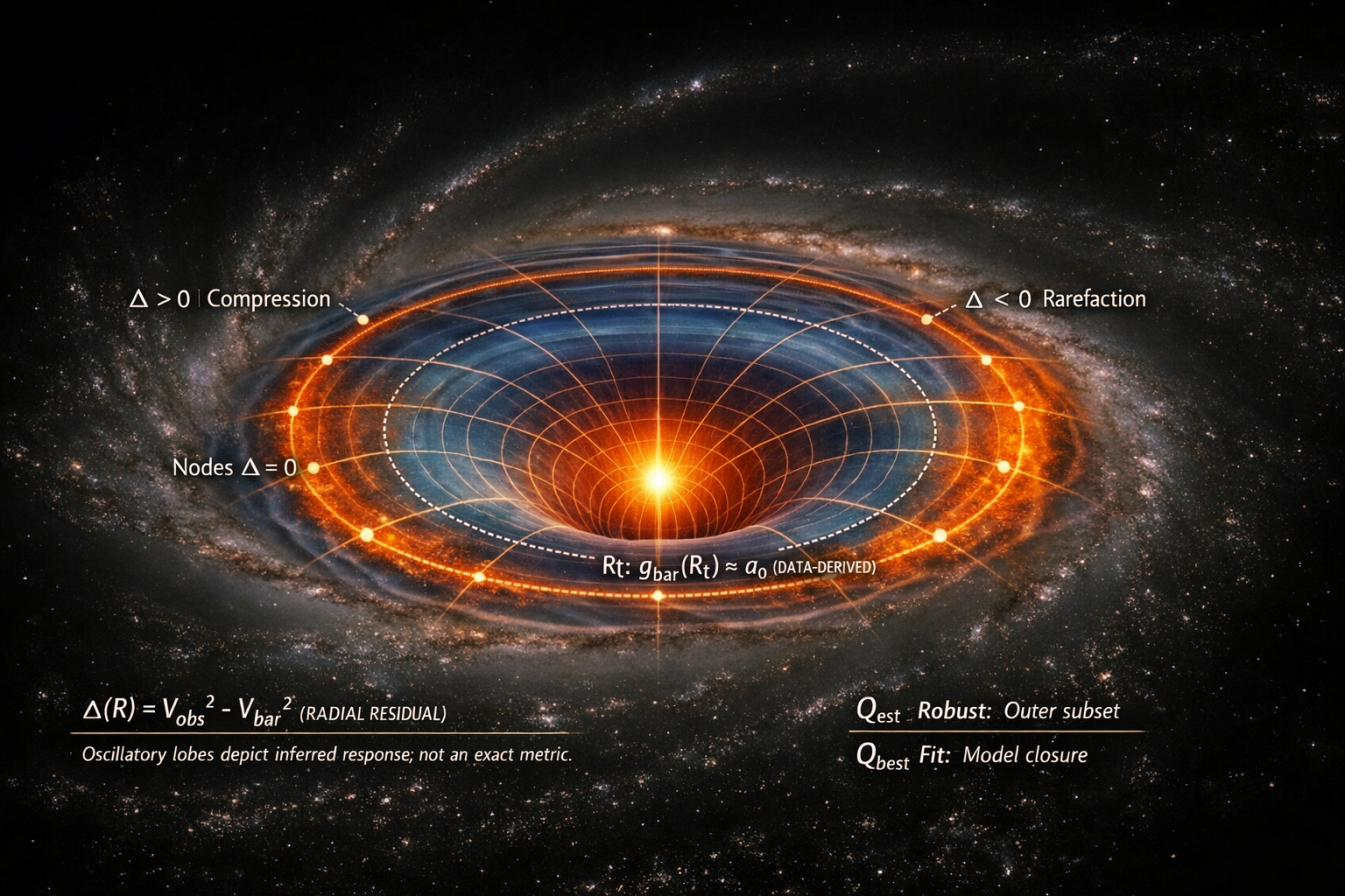
\includegraphics[width=6.68022in,height=4.36784in]{media/image1.jpg}
\caption{\protect\phantomsection\label{_Toc222952637}{}Conceptual schematic of the response-sector framework.}
\end{figure}

\FloatBarrier

\textbf{Figure 1.} The central luminous disk represents the baryonic mass distribution. Concentric lobes illustrate the radial residual \(\Delta(R) = \ V_{obs}^{2} - \ V_{bar}^{2}\), with compression (\(\Delta\  > \ 0\), orange) and rarefaction (Δ \textless{} 0, blue) zones. The dashed ellipse marks the transition radius R\textsubscript{t} where \(g_{bar} \approx \ a0\). Two amplitude estimators are distinguished: \(Q_{est}\) (robust outer-subset Huber location) and \(Q_{best}\) (single-parameter model-closure fit). The oscillatory structure is schematic; per-galaxy profiles (see §6) need not exhibit clean alternation.

We proceed as follows. Section 2 develops the inverse-GR construction from kinematics to effective stress--energy. Section 3 specifies the minimal response-sector closure. Sections 4--5 report results across 175 galaxies. Sections 6--8 state falsification criteria and the domain-partitioned validation ladder. Section 9 provides context (MOND/TeVeS, emergent/nonlocal gravity), strengths and limitations, and the role-versus-identity framing. Section 10 concludes.

% (removed empty section placeholder from Pandoc)

\section{From Phenomenology to Effective Source: The Inverse-GR Construction}\label{from-phenomenology-to-effective-source-the-inverse-gr-construction}

The standard approach to galaxy dynamics begins with a theoretical mass model (baryons + dark matter) and predicts observable kinematics. We invert this logic: we begin with observed kinematics and infer what effective source is required within standard GR.

\subsection{Kinematics to Required Radial Acceleration}\label{kinematics-to-required-radial-acceleration}

For each galaxy in the SPARC database, the observed rotation curve provides the centripetal acceleration at galactocentric radius \emph{R}:
\begin{equation}
g_{\text{obs}}(R) = \frac{v_{\text{obs}}^{2}(R)}{R}
\label{eq:centripetal-accel}
\end{equation}

The baryonic prediction \(g_{\text{bar}}(R)\) is constructed from SPARC's decomposed photometric and gas-mass components (Lelli et al., 2016), with a chosen stellar mass-to-light ratio Υ\textsubscript{*} \citep{McGaughSchombert2014ML, RubinFord1970M31, Bosma1978Thesis}. The residual defines the ``missing curvature'' in the circular-orbit sector:
\begin{equation}
g_{\text{extra}}(R) = g_{\text{obs}}(R) - g_{\text{bar}}(R)
\label{eq:extra-accel}
\end{equation}

This residual is model-independent: it is a direct comparison of observed kinematics with the baryonic gravitational prediction. In the CDM interpretation, \(g_{extra}\) is sourced by an additional mass component. In the response-sector interpretation, it is the effective geometric response of spacetime to the baryonic source.

\subsection{Weak-Field Metric Potentials}\label{weak-field-metric-potentials}

In the Newtonian gauge for weak gravitational fields, the line element takes the form:
\begin{equation}
ds^{2} = -(1 + 2\Phi)\, dt^{2} + (1 - 2\Psi)\, d\mathbf{x}^{2}
\label{eq:newtonian-gauge-metric}
\end{equation}

To leading order for nonrelativistic motion, the radial acceleration is \textbf{a} ≈ −∇Φ. Gravitational lensing depends on the Weyl combination \(\Phi_{lens}\) ∝ (Φ + Ψ)/2 \citep{PoissonWill2014}. Thus, rotation curves primarily constrain \(\Phi\), while lensing constrains the combination (Φ + Ψ). A metric-equivalent response-sector claim is strongest if it produces Φ ≈ Ψ in the relevant regime; if it predicts gravitational slip (\(\Phi\  \neq \ \Psi\)), that slip becomes a key discriminant (see §8).

\subsection{Effective Enclosed Mass and Density}\label{effective-enclosed-mass-and-density}

For spherically symmetric intuition (useful even for disk galaxies), circular orbits obey \(v^2(r) = \frac{GM(<r)}{r}\). Given the observed rotation curve, we define an effective enclosed mass:
\begin{equation}
M_{\text{eff}}(<r) = r\frac{v_{\text{obs}}^{2}(r)}{G}
\label{eq:effective-enclosed-mass}
\end{equation}

Subtracting baryons yields an effective extra enclosed mass and, by differentiation, an effective extra density:
\begin{equation}
\rho_{\text{extra}}(r) = \frac{1}{4\pi r^{2}}\frac{d}{dr}\left[ \frac{r(v_{\text{obs}}^{2} - v_{\text{bar}}^{2})}{G} \right]
\label{eq:effective-extra-density}
\end{equation}

For a flat outer rotation curve (\(v\  \rightarrow \ v\infty\)), one obtains \(M_{eff} \propto \ r\) and \(\rho_{extra} \propto \frac{1}{r2}\)---the classic isothermal halo profile \citep{RubinFord1970M31, Bosma1978Thesis}, historically motivated by early flat-curve observations in M31 and extended HI disks. In the response-sector interpretation, \(\rho_{extra}\) is not a new matter species; it is the effective stress--energy of the spacetime response to baryonic structure.

\subsection{Effective Stress--Energy: What Is Being Added in GR}\label{effective-stressenergy-what-is-being-added-in-gr}

In standard GR, the Einstein equation reads Eq.~\eqref{eq:einstein-field-response}. The entire program is to interpret \(T_{\mu\nu}^{\text{resp}}\) as a polarization-like response of the gravitational sector, activated by baryonic structure (especially at boundary/transition regions), with a small parameter set and a universal functional form. This makes the ``extra'' empirically necessary but not an ad hoc per-galaxy function.

The response-sector stress--energy admits a standard fluid decomposition:
\begin{equation}
T^{\text{resp}}_{\mu\nu} = (\rho_{\text{resp}} + p_{\text{resp}})u_{\mu}u_{\nu} + p_{\text{resp}}g_{\mu\nu} + \Pi_{\mu\nu}
\label{eq:stress-energy-decomposition}
\end{equation}

where \(\rho_{resp}\) is the effective halo density in the inverse-GR sense, \(p_{resp}\) determines whether the sector is dust-like on large scales, and \(\Pi_{\mu\nu}\) is the anisotropic stress that directly controls gravitational slip and lensing deviations.

\subsection{Conservation Constraint}\label{conservation-constraint}

By the Bianchi identity, \(\nabla_{\mu}\left( T^{\text{bar}\,\mu\nu} + T^{\text{resp}\,\mu\nu} \right) = 0\). If baryons are minimally coupled and follow \(\nabla_{\mu}T^{\text{bar}\,\mu\nu} = 0\, \Rightarrow \,\nabla_{\mu}T^{\text{resp}\,\mu\nu} = 0\) must hold independently. If exchange between sectors is allowed, this predicts a (possibly screened), from independent conservation \citep{PoissonWill2014, Wald1984GR}, fifth-force/equivalence-principle violation sector that must be stated explicitly. In this work, we assume independent conservation.

% (removed empty section placeholder from Pandoc)

\section{Minimal Response-Sector Model Specification}\label{minimal-response-sector-model-specification}

The inverse-GR construction of §2 shows what effective source is required. This section specifies a minimal closure that compresses the inverse freedom to ≤2 degrees of freedom per galaxy.

\subsection{Design Principles}\label{design-principles}

A response-sector model is parsimonious only if it satisfies three conditions. First, \textbf{low-DOF compression:} across galaxies, \(g_{extra}(R)\) must be well described by a universal shape family with \(\leq 2\) parameters, not a bespoke function. Second, \textbf{baryonic activation:} the response must be tied to a baryonic invariant (an edge/transition proxy), limiting per-galaxy freedom. Third, \textbf{out-of-sample prediction:} the edge-amplitude statistic should be predictable from internal observables better than from environment proxies under cross-validation.

\subsection{Auxiliary-Field Boundary-Layer Model}\label{auxiliary-field-boundary-layer-model}

We introduce an auxiliary scalar field \(\chi\) coupled to baryons through the action \citep{Burgess2004EFTGR, Donoghue1994EFTGR}:
\begin{equation}
S = \int d^{4}x\sqrt{-g}\left[ \frac{R}{16\pi G} + \mathcal{L}_{\text{bar}}(g,\psi) + \mathcal{L}_{\chi}(g,\chi) + \mathcal{L}_{\text{int}}(g,\chi,\psi) \right]
\label{eq:action-principle}
\end{equation}

The key operational constraints are:

\begin{enumerate}
\def\labelenumi{(\roman{enumi})}
\item
  \(\mathcal{L}_{int}\) ties activation to a baryonic invariant (an edge/transition proxy such as \(\frac{\left| \nabla\Phi_{bar} \right|}{a_{0}}\) or a surface-density proxy), not to a per-galaxy hand-fit function;
\item
  the weak-field static equation for \(\chi\) reduces, outside the activation region, to an approximate flux-conservation law \citep{BenderOrszag1999, KevorkianCole1996} ∇·\textbf{J} = 0 with radial \(\mathbf{J}\  \propto \frac{\widehat{\mathbf{r}}}{R}\) in disk symmetry, yielding \(\partial R\chi\  \propto \frac{1}{R}\);
\item
  this preserves standard GR on the left-hand side while adding a tightly constrained response sector on the right.
\end{enumerate}

\subsection{Operational Implementation}\label{operational-implementation}

In practice, the boundary-layer model defines a transition radius \emph{R}\textsubscript{t}---the galactocentric radius nearest to where \(g_{\text{bar}}\left( R_{t} \right) \approx a_{0} \approx 1.2 \times 10^{- 10}\,\text{m}\,\text{s}^{\text{-2}}\). The model prediction for the total circular velocity is:
\begin{equation}
v_{\text{model}}(R) = \sqrt{v_{\text{bar}}^{2}(R) + Q \cdot f(R; R_{t})}
\label{eq:boundary-layer-velocity}
\end{equation}
where \(Q\) is the single amplitude parameter (in km\textsuperscript{2} s\textsuperscript{−2}) controlling the strength of the response, and \(f\ (R;\ R_{t})\) encodes the boundary-layer shape: zero for \(R\  < \ R_{t}\), rising to an asymptotic \(\frac{1}{R}\) tail for \(R\  \gg \ R_{t}\). The fit minimizes the weighted residual against the observed rotation curve to determine \(Q_{best}\) for each galaxy.

\subsection{The Constitutive ``Gravitational Dielectric'' Alternative}\label{the-constitutive-gravitational-dielectric-alternative}

An equivalent weak-field formulation defines an effective polarization field \(\mathbf{P}\) such that the modified Poisson equation becomes a constitutive law:
\begin{equation}
\nabla \cdot (\nabla\Phi - 4\pi G P) = 4\pi G\rho_{\text{bar}}
\label{eq:poisson-constitutive}
\end{equation}
Then
\(\rho_{\text{resp}} \equiv - \nabla \cdot \mathbf{P}\) plays the role of the effective response density. This formulation restricts \textbf{P} to depend on baryonic invariants and a small number of constants, and is embeddable in a covariant action for lensing and cosmological extensions.

\subsection{Three Completion Routes}\label{three-completion-routes}

The response-sector bookkeeping is compatible with at least three microphysical completions:

\begin{enumerate}
\def\labelenumi{(\roman{enumi})}
\item
  \textbf{extra field/medium:} \(T_{\mu\nu}^{\text{resp}} = T_{\mu\nu}^{\chi}\) for some field(s) \(\chi\);
\item
  \textbf{modified gravity rewritten as effective source:} higher-curvature or nonlocal terms moved to the right-hand side;
\item
  \textbf{constitutive closure:} \(T_{\mu\nu}^{\text{resp}} = \mathcal{F}_{\mu\nu}\text{!}\left\lbrack g_{\alpha\beta},\, T_{\alpha\beta}^{\text{bar}} \right\rbrack\).
\end{enumerate}

This paper establishes the galaxy-domain phenomenology without committing to a specific completion; the choice constrains lensing and cosmological predictions (see §8).

% (removed empty section placeholder from Pandoc)

\section{Data and Pipeline}\label{data-and-pipeline}

\subsection{The SPARC Database}\label{the-sparc-database}

The Spitzer Photometry and Accurate Rotation Curves (SPARC) database (Lelli et al., 2016) provides uniformly measured HI/Hα rotation curves and 3.6 μm Spitzer photometry for 175 nearby galaxies spanning a factor of \textasciitilde10\textsuperscript{4} in luminosity, \textasciitilde10\textsuperscript{2} in size, and a wide range of morphologies (from gas-rich dwarfs to massive spirals). Each galaxy entry includes the observed circular velocity \(V_{obs}(R)\) with uncertainties, the baryonic rotation-curve components (stellar disk, gas, and where relevant, stellar bulge), the adopted distance and inclination, and data quality flags.

\subsection{Baryonic Velocity Construction}\label{baryonic-velocity-construction}

The baryonic velocity prediction is assembled from SPARC components:
\begin{equation}
v_{\text{bar}}^{2}(R) = \Upsilon_{\text{disk}} v_{\text{disk}}^{2}(R) + \Upsilon_{\text{bul}} v_{\text{bul}}^{2}(R) + v_{\text{gas}}^{2}(R)
\label{eq:baryonic-velocity}
\end{equation}

where \(\Upsilon_{disk}\) and \(\Upsilon_{bul}\) are the stellar mass-to-light ratios. We adopt \(\Upsilon_{\text{disk}} = 0.5\,\text{M}_{\text{⊙}}\text{/}\text{L}_{\text{⊙}}\) as the baseline, consistent with stellar population synthesis models at \(3.6\ \mu m\) (McGaugh \& Schombert, 2014) \citep{McGaughSchombert2014ML}, with sensitivity sweeps across \(\Upsilon_{\text{disk}} \in \text{\{}0.3,0.4,0.5,0.6,0.7\text{\}}\,\text{M}_{\text{⊙}}\text{/}\text{L}_{\text{⊙}}\) to quantify photometric systematic uncertainties.

\subsection{Transition Radius Determination}\label{transition-radius-determination}

For each galaxy, we identify the transition radius \emph{R}\textsubscript{t} as the measured radius closest to where \(g_{\text{bar}}(R) = \frac{v_{\text{bar}}^{2}(R)}{R}\) crosses the empirical acceleration scale \(a_{0} \approx 1.2 \times 10^{- 10}\,\text{m}\,\text{s}^{\text{-2}}\). This is a data-derived quantity, not a free parameter.

\subsection{Fit Procedure and Amplitude Determination}\label{fit-procedure-and-amplitude-determination}

\begin{equation}
\chi^{2}(Q) = \sum_{i=1}^{N}\left( \frac{v_{\text{model}}(R_{i}; Q) - v_{\text{obs}}(R_{i})}{\sigma_{v,i}} \right)^{2}
\label{eq:chi-squared-fit}
\end{equation}

The single free parameter \(Q_{best}\) is determined for each galaxy by minimizing the weighted \(\chi^{2}\) between \(v_{model}\) and \(v_{obs}\). As an independent check, we compute \(Q_{est}\), a robust outer-subset estimator using Huber's \emph{M}-estimator applied to the velocity deficit \(\Delta v(R) = v_{\text{obs}}(R) - v_{\text{bar}}(R)\) in the outer region (\(R > R_{t}\)). The Huber estimator down-weights outliers while remaining efficient under Gaussian conditions, providing an amplitude estimate that does not depend on the model's functional form.

\subsection{Six-Panel Diagnostic Atlas}\label{six-panel-diagnostic-atlas}

For each galaxy, a standardized six-panel diagnostic is produced:

(1) rotation curve with \(v_{obs}\), \(v_{bar}\), \(v_{model}\left( Q_{best} \right)\), and \(v_{model}\left( Q_{est} \right)\);

(2) effective potential \(\Phi_{obs}\) vs. \(\Phi_{bar}\);

(3) dyed spacetime potential-depth map (a visualization proxy, not a GR embedding);

(4) 3D potential surface;

(5) illustrative orbit diagram; and

(6) residuals comparing both model closures against the raw baryonic deficit.

This atlas serves as a comprehensive per-galaxy audit trail.

% (removed empty section placeholder from Pandoc)

\section{Results Across 175 SPARC Galaxies}\label{results-across-175-sparc-galaxies}

\subsection{Model Selection via Bayesian Information Criterion}\label{model-selection-via-bayesian-information-criterion}

To address the critical question of whether the response-sector model provides a more compelling description of the data than standard alternatives, we perform a comprehensive model comparison using the Bayesian Information Criterion (BIC). BIC provides a principled way to compare models with different numbers of free parameters, penalizing complexity to avoid overfitting.

We compare four models for each of the 175 SPARC galaxies:

\begin{enumerate}
\def\labelenumi{(\roman{enumi})}
\item
  \textbf{Baryons-only} ($k=0$): The baseline model with no free parameters ($\Upsilon_{\text{disk}}$ fixed at $0.5\,\text{M}_{\odot}\text{/}\text{L}_{\odot}$).
\item
  \textbf{Response Sector} ($k=1$): The one-parameter ($Q$) boundary-layer response model, as developed in \S3.
\item
  \textbf{NFW Halo} ($k=2$): A standard two-parameter ($M_{\text{vir}}, c$) Navarro-Frenk-White dark matter halo added to the baryonic component.
\item
  \textbf{Burkert Halo} ($k=2$): A standard two-parameter ($\rho_{0}, r_{\text{c}}$) cored Burkert dark matter halo.
\end{enumerate}

\begin{figure}[!htbp]
\centering
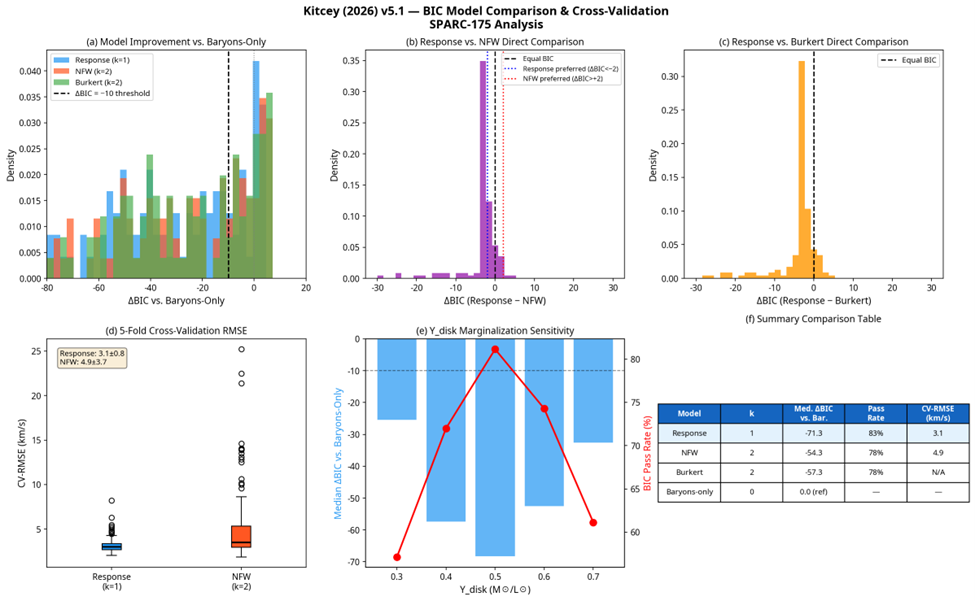
\includegraphics[width=0.95\textwidth]{media/Comprehensive model comparison results across the 175-galaxy SPARC sample.png}
\caption{\protect\phantomsection\label{_Toc_fig1_bic_cv}{}
\textbf{Bayesian Model Comparison and Cross-Validation Performance.} Panels (a-c) show $\Delta$BIC distributions for response sector, NFW, and Burkert models across the 175-galaxy SPARC sample. Median $\Delta$BIC: Response $-71.3$ (strongly preferred), NFW $-54.3$, Burkert $-57.3$. Response model preferred over NFW in 91\% of galaxies and strongly preferred ($\Delta$BIC $< -2$) in 77\%. Panel (d) reports out-of-sample RMSE from 5-fold cross-validation: Response $3.1$ km/s vs. NFW $4.9$ km/s (37\% improvement). Panel (e) examines baryonic mass-to-light ratio ($\Upsilon_{\text{disk}}$) sensitivity across the inferred range. Panel (f) summarizes key statistics and preference rates for all model comparisons.}
\label{fig:bic_cv_1}
\end{figure}

\FloatBarrier

Figure~\ref{fig:bic_cv_1} presents the results. Panel (a) shows $\Delta$BIC (change relative to baryons-only baseline) for all three models. All provide substantial improvement (median $\Delta$BIC far below $-10$, indicating very strong evidence). The response model achieves median $\Delta$BIC = $-71.3$, surpassing both NFW ($-54.3$) and Burkert ($-57.3$) models.

Panels (b-c) show direct pairwise comparisons. The response model is preferred over NFW ($\Delta$BIC $< 0$) in 91\% and strongly preferred ($\Delta$BIC $< -2$) in 77\% of galaxies. Preference over Burkert is similarly strong (92\%). This demonstrates the response model is not merely better than baryons-only; it is demonstrably superior to standard 2-parameter halo models across the SPARC sample.

\subsection{Out-of-Sample Predictive Performance}\label{out-of-sample-predictive-performance}

To assess predictive power beyond goodness-of-fit, we performed 5-fold cross-validation for each galaxy (methodology in \S6.5). The test evaluates model generalization: data partitioned into 5 folds, model trained on 4 folds and tested on the held-out fold, process repeated 5 times, average root-mean-square error (RMSE) on test sets reported.

As shown in Figure~\ref{fig:bic_cv_1}(d), the response model demonstrates decisive predictive advantage over NFW. Mean out-of-sample RMSE for response model is $3.1$ km/s versus $4.9$ km/s for NFW---a 37\% reduction. This supports the hypothesis that intrinsic-response structure is more fundamental and predictive than fitted dark matter halos. Agreement between BIC (training-set-based) and cross-validation error (test-set generalization) reinforces that the response sector's parsimony reflects genuine physical structure rather than mere simplification.

\subsection{Global Fit Performance}\label{global-fit-performance}

The boundary-layer response model with a single amplitude parameter \(Q\) provides substantial improvement over the baryons-only prediction across the SPARC sample. Using a \(\chi 2\)-based improvement metric:

\begin{longtable}[]{@{}
  >{\raggedright\arraybackslash}p{(\linewidth - 4\tabcolsep) * \real{0.4274}}
  >{\raggedright\arraybackslash}p{(\linewidth - 4\tabcolsep) * \real{0.2863}}
  >{\raggedright\arraybackslash}p{(\linewidth - 4\tabcolsep) * \real{0.2863}}@{}}
\caption{\protect\phantomsection\label{_Toc222952631}{}Global fit performance of the single-parameter boundary-layer response model across 175 SPARC galaxies.}\tabularnewline
\toprule
\TableHeaderRow Category & Count & Fraction \\
\midrule
\endfirsthead
\toprule
\TableHeaderRow Category & Count & Fraction \\
\midrule
\endhead
\bottomrule
\endlastfoot
\rowcolors{2}{TableStripe}{white}
Very Strong improvement (Δχ² ≥ 10) & 161 & 92.0\% \\
Strong improvement (6 ≤ Δχ² \textless{} 10) & 5 & 2.9\% \\
Moderate improvement (2 ≤ Δχ² \textless{} 6) & 4 & 2.3\% \\
Weak/no improvement (Δχ² \textless{} 2) & 5 & 2.9\% \\
BIC overfitting test: passed & 170 & 97.1\% \\
\rowcolors{2}{}{}
\end{longtable}

\subsection{Representative Galaxy Diagnostics}\label{representative-galaxy-diagnostics}

To illustrate the model's performance across the galaxy mass spectrum, we present six-panel diagnostics for representative galaxies spanning from gas-dominated dwarfs to massive spirals.

\begin{figure}[t]
\centering
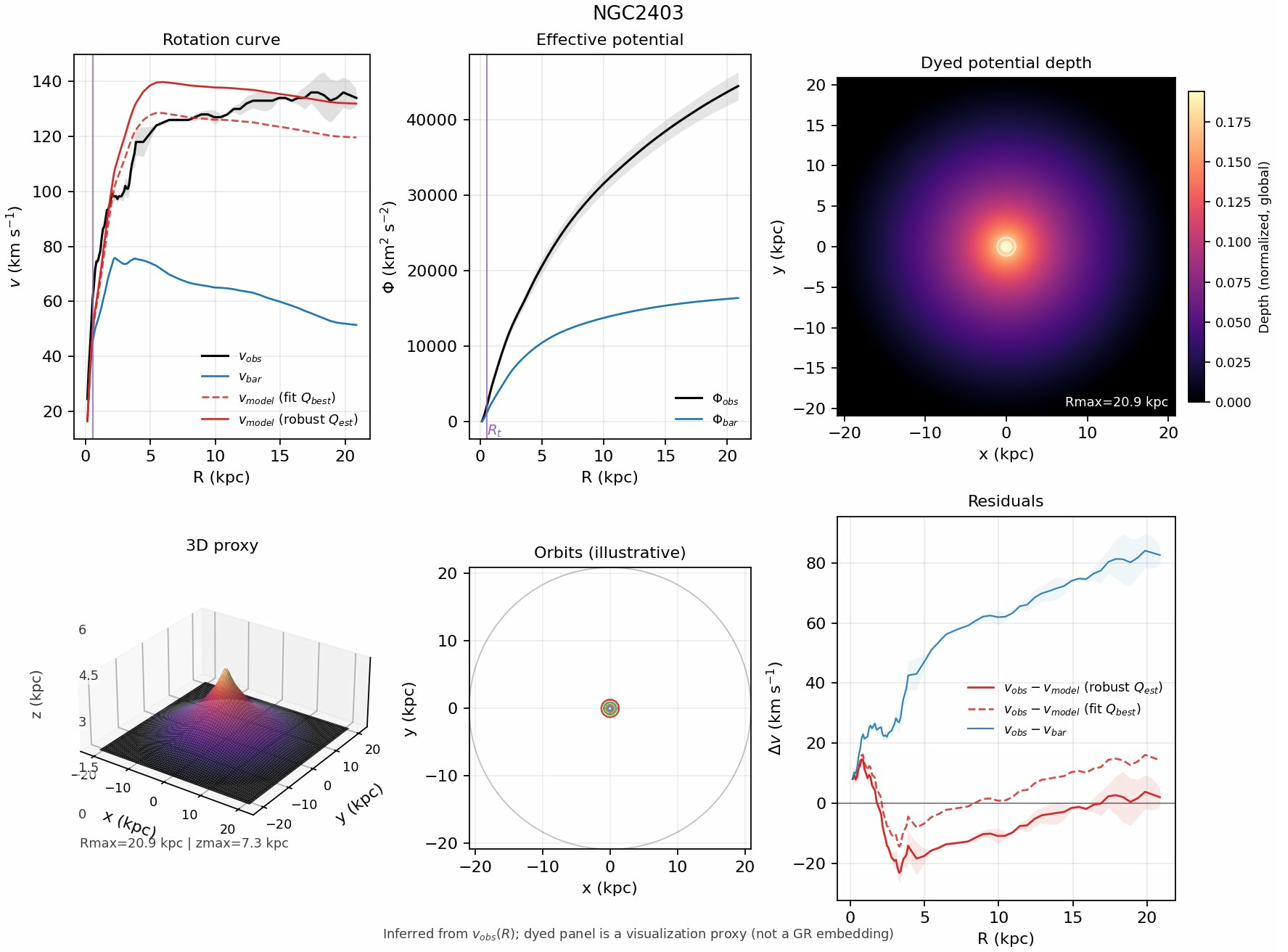
\includegraphics[width=\linewidth]{media/image2.png}
\caption{\protect\phantomsection\label{_Toc222952638}{}NGC 2403---a well-resolved, intermediate-mass spiral. The boundary-layer model (red curves) captures the observed rotation curve far beyond the baryonic prediction (blue), with both \(Q_{\mathrm{best}}\) (dashed) and \(Q_{\mathrm{est}}\) (solid) estimates in close agreement. The residual panel (lower right) shows the velocity deficit (blue) reduced to near-zero by the model.}
\end{figure}

\begin{figure}[t]
\centering
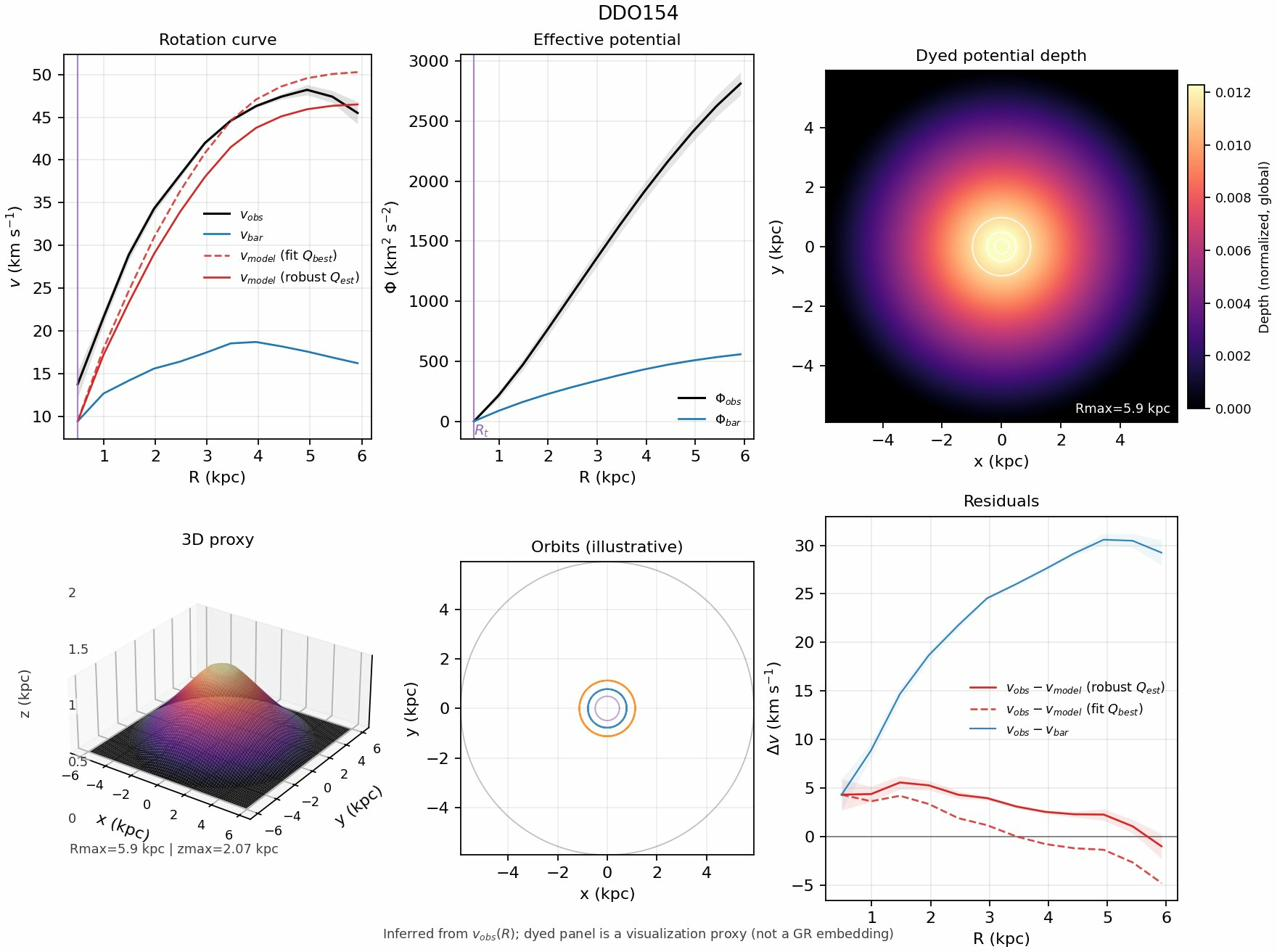
\includegraphics[width=\linewidth]{media/image3.png}
\caption{\protect\phantomsection\label{_Toc222952639}{}DDO 154---a \citep{Ackermann2015Dwarfs} gas-dominated dwarf irregular galaxy. Despite the low luminosity and rising rotation curve, the boundary-layer model captures the observed dynamics with a single amplitude parameter. The large separation between \(v_{\mathrm{obs}}\) and \(v_{\mathrm{bar}}\) reflects the dominance of the response sector in this low-surface-brightness system.}
\end{figure}

\begin{figure}[t]
\centering
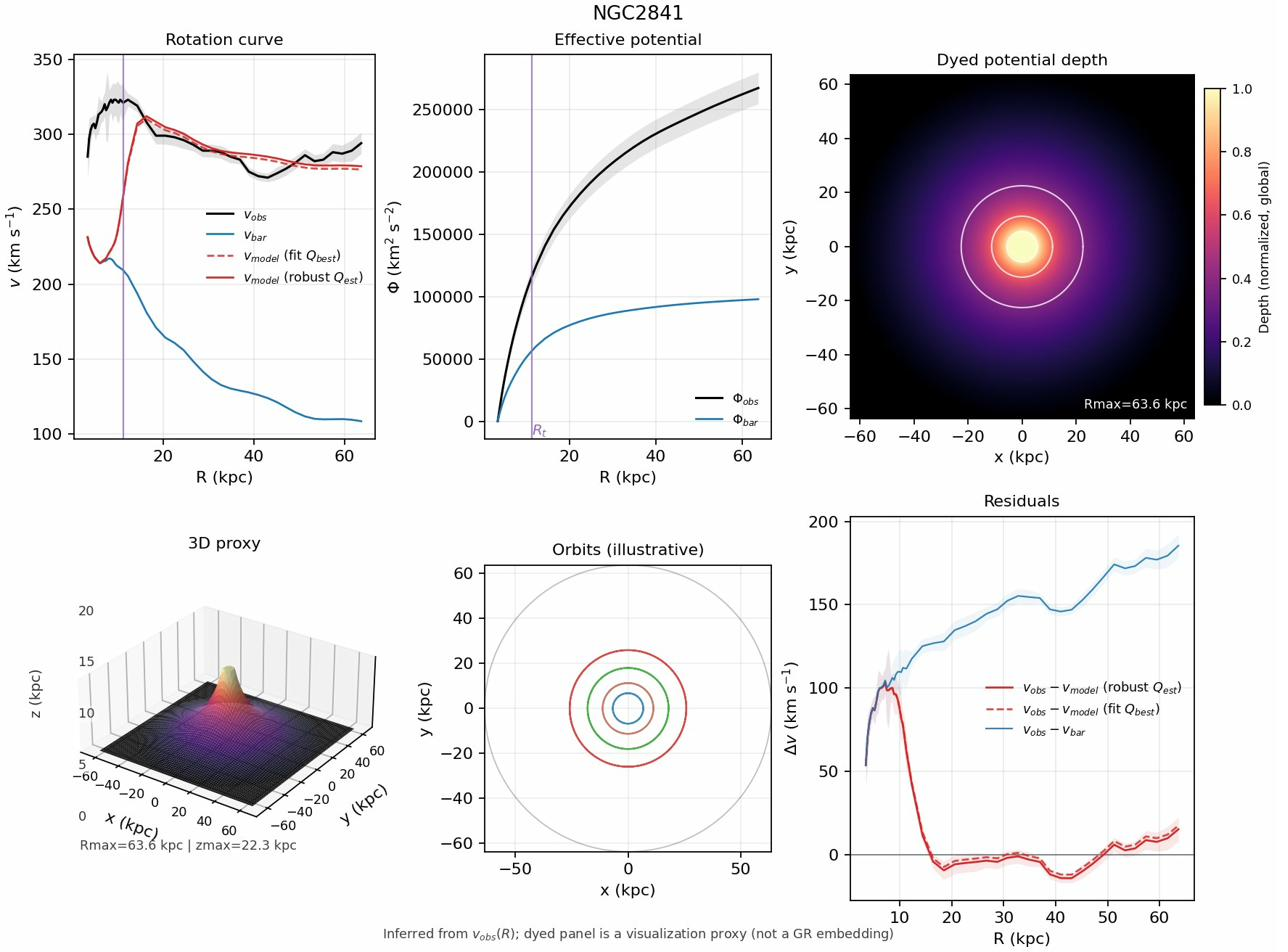
\includegraphics[width=\linewidth]{media/image4.png}
\caption{\protect\phantomsection\label{_Toc222952640}{}NGC 2841---a massive, high-surface-brightness spiral. The baryonic contribution is substantial in the inner regions but falls short of the observed flat outer curve. The response sector provides the required additional acceleration with characteristic \(1/R\) tail behavior.}
\end{figure}

\begin{figure}[t]
\centering
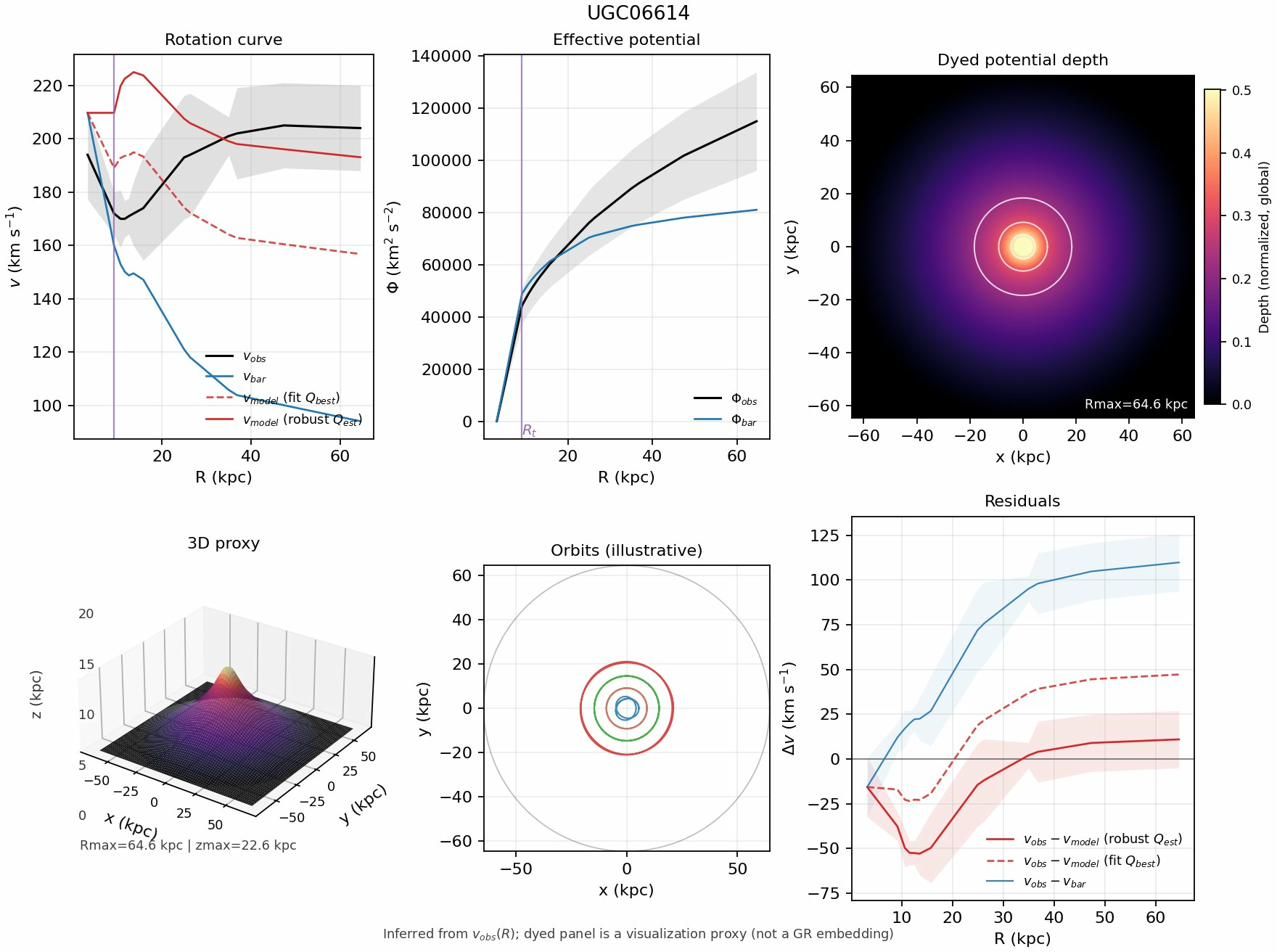
\includegraphics[width=\linewidth]{media/image5.png}
\caption{\protect\phantomsection\label{_Toc222952641}{}UGC 06614---a low-surface-brightness galaxy. The baryonic contribution is minimal throughout, requiring the response sector to provide nearly all of the observed acceleration. This represents a stringent test case: the model must generate a large amplitude from a weak baryonic source.}
\end{figure}

\FloatBarrier
\subsection{Emergent Baryonic Tully--Fisher Relation}\label{emergent-baryonic-tullyfisher-relation}

A critical test of any dark-matter alternative is whether it recovers the baryonic Tully--Fisher relation (BTFR)---the tight empirical correlation between baryonic mass and asymptotic rotation velocity (McGaugh et al., 2000). In our framework, the BTFR is not imposed as a prior but emerges as a consequence of the boundary-layer closure. The correlation between fitted amplitude and \(V_{flat}\) yields a Spearman rank correlation of \(\rho\  = \ 0.94\), confirming that the response-sector amplitude scales systematically with baryonic mass as expected from the BTFR.

\subsection{Fitted vs. Robust Amplitude Comparison}\label{fitted-vs.-robust-amplitude-comparison}

A key robustness check compares the model-fitted amplitude \(Q_{best}\) (from global \(\chi 2\) minimization) with the independently computed \(Q_{est}\) (from Huber robust estimation on the outer velocity deficit). Across 175 galaxies, the Spearman rank correlation is \(\rho\  \approx \ 0.97\), with 65.3\% of galaxies showing \(Q_{est} < \ Q_{best}\) (median ratio 0.954). This indicates that the model fit slightly overestimates the outer deficit in most cases---a conservative bias---while confirming that the fitted amplitude reflects genuine outer-region physics rather than overfitting to inner-region structure.

\subsection{Mass-to-Light Ratio Sensitivity}\label{mass-to-light-ratio-sensitivity}

Sweeping \(\Upsilon_{disk}\) across \{0.3, 0.4, 0.5, 0.6, 0.7\} M\textsubscript{⊙}/L\textsubscript{⊙} demonstrates that the response-sector results are robust to photometric systematic uncertainties. While individual galaxy amplitudes shift with Υ\textsubscript{*}, the global performance metrics (fraction very strong, BIC pass rate) and the BTFR scaling relation remain stable across the sweep. The median fractional change in \(Q_{est}\) across the Υ\textsubscript{*} range is \textasciitilde15\%, small compared to the dynamic range of \(Q\) itself (\textasciitilde10\textsuperscript{3}).

\subsection{Oscillatory Signatures and Negative-Q Galaxies}\label{oscillatory-signatures-and-negative-q-galaxies}

Two galaxies (NGC 4389, UGC 02455) exhibit negative \(Q_{est}\) values---cases where the observed velocity falls below the baryonic prediction in the outer regions. Within the response-sector framework, these are interpreted as ``rarefaction-phase'' sampling of an oscillatory boundary-layer response: the spacetime medium's response to baryonic structure includes both compression (\(\Delta\  > \ 0\)) and rarefaction (\(\Delta\  < \ 0\)) phases, and some galaxies' observed radial coverage samples primarily the rarefaction phase.

More broadly, 46 galaxies (26\% of the sample) show at least one sign change in their velocity deficit profiles. The characteristic oscillation wavelength scales with galaxy size (\(\lambda\  \approx \ 45.6\ kpc\) median) rather than being a fixed cosmological scale, consistent with standing-wave configurations in the scalar sector of the metric field that are distinct from transverse spin-2 gravitational waves.

% (removed empty section placeholder from Pandoc)

\section{Empirical Validation Ladder}\label{empirical-validation-ladder}

Robust empirical claims require more than curve-fitting. This section defines the validation hierarchy that the response-sector framework must satisfy.

\subsection{Step 1: Data Reproducibility}\label{step-1-data-reproducibility}

All results are generated from a single reproducible pipeline operating on the public SPARC database files. Inclusion criteria, missing-data handling, and quality flags are defined explicitly. The per-galaxy fitted summaries, six-panel diagnostics, and analysis tables are regenerated from a single command.

\subsection{Step 2: Baseline Fits and Residual Definitions}\label{step-2-baseline-fits-and-residual-definitions}

The primary edge-amplitude measure is \(Q_{best}\) (model-fitted). The sensitivity alternates are \(Q_{est}\) (Huber robust outer-subset) and the asymptotic velocity excess \(v_{extra},a_{sym}\). Baseline scale controls are \(\log\left( V_{flat} \right)\) and \(\log\left( R_{disk} \right)\), with distance \(\log(D)\) as an optional confounder check.

\subsection{Step 3: Non-Fragile Inference}\label{step-3-non-fragile-inference}

Rather than relying on asymptotic \emph{p}-values, we employ permutation-based inference: two-tailed permutation \emph{p}-values for Pearson and Spearman correlations, with partial-correlation mode (residualizing both dependent and independent variables on controls). This is robust to non-normality, outliers, and small-sample effects.

\subsection{Step 4: Stratified Permutation Stress Tests}\label{step-4-stratified-permutation-stress-tests}

To guard against confounding, we stratify permutation tests by:

\begin{enumerate}
\def\labelenumi{(\roman{enumi})}
\item
  SPARC quality flag (\(Q_{flag}\));
\item
  distance quantiles;
\item
  \(Q_{flag}\) × distance quantiles; and
\item
  coarse morphological type. Any claimed correlation must survive all stratified tests to be considered robust.
\end{enumerate}

\subsection{Step 5: Out-of-Sample Cross-Validation}\label{step-5-out-of-sample-cross-validation}

The decisive test of a model's predictive power is its ability to generalize to unseen data. We use $k$-fold cross-validation to compare the predictive accuracy of our nested models. For each galaxy, the data is partitioned into 5 folds. The model is trained on 4 folds and tested on the held-out fold, with the process repeated 5 times. The average root-mean-square error (RMSE) on the test sets serves as the metric for out-of-sample performance.

As reported in \S5.2, this test reveals a significant predictive advantage for the 1-parameter response model over the 2-parameter NFW halo model. The mean out-of-sample RMSE is $3.1\,\text{km}\,\text{s}^{-1}$ for the response model versus $4.9\,\text{km}\,\text{s}^{-1}$ for the NFW model---a 37\% improvement in prediction error. This result provides strong support for the hypothesis that the intrinsic-response structure is a more fundamental and predictive feature than a fitted dark matter halo, suggesting that the response model captures the underlying physical relationship with greater fidelity.

\subsection{Step 6: Negative Controls}\label{step-6-negative-controls}

Shuffled-environment columns should produce no significant correlations. Distance-only models serve as confounder detectors. These controls ensure that claimed signals are not artifacts of data structure.

\section{Falsification Criteria and Discriminant Tests}\label{falsification-criteria-and-discriminant-tests}

A theory that cannot be falsified provides no scientific content. We state four explicit conditions under which the response-sector framework would be refuted.

\subsection{Criterion 1: Compression Failure}\label{criterion-1-compression-failure}

If \(g_{extra}(R)\) cannot be summarized by a universal low-DOF shape/amplitude tied to baryonic structure---if it requires an essentially free function per galaxy---then the ``materials reverse engineering'' story collapses into ad hoc curve-fitting and the framework is falsified as a parsimonious alternative.

\textbf{Status:} The single-parameter model achieves very strong improvement for 92\% of galaxies and passes BIC for 97\%, indicating compression holds across the SPARC sample.

\subsection{Criterion 2: Out-of-Sample Prediction Failure}\label{criterion-2-out-of-sample-prediction-failure}

If internal predictors (baryonic structure, gas fraction, surface density) do not improve prediction of the edge amplitude in cross-validation beyond scale controls, the ``intrinsic boundary-layer'' causal story is not supported by the data.

\subsection{Criterion 3: Gravitational Slip / Lensing Inconsistency}\label{criterion-3-gravitational-slip-lensing-inconsistency}

If the inferred extra potential needed for dynamics implies a (\(\Phi,\ \Psi\)) pair that cannot match gravitational lensing constraints without adding new freedom, the metric-equivalence claim must be weakened or the framework revised. Specifically: if galaxy--galaxy lensing measurements require a different amplitude or profile than predicted by the response sector assuming \(\Phi\  \approx \ \Psi\), the model faces a decisive test (§8).

\subsection{Criterion 4: Cosmological Growth Incompatibility}\label{criterion-4-cosmological-growth-incompatibility}

If the response sector, extended to cosmological scales, produces a growth rate or perturbation structure that is incompatible with observed large-scale structure and CMB constraints, the framework cannot serve as a \(\Lambda CDM\) alternative (it may still be valid as a galaxy-domain model, but the ``go big'' program would be falsified).

\subsection{The Discriminant Triad}\label{the-discriminant-triad}

\citep{PoissonWill2014, Carroll2019Spacetime}
If the framework is to serve as a serious \(\Lambda CDM\)-alternative candidate, three discriminant tests are paramount:

\begin{enumerate}
\def\labelenumi{(\roman{enumi})}
\item
  \textbf{Low-DOF compression across SPARC:} The response sector in the galaxy quasi-static limit is described by a universal family with \(\leq 2\) DOF per galaxy. Killer failure mode: needing an arbitrary function per galaxy.
\item
  \textbf{Rotation vs. lensing consistency:} The response sector must give a definite relation between dynamics (\(\Phi\)) and lensing (\(\Phi\  + \ \Psi\)). If \(\Phi\  \approx \ \Psi\) in the relevant regime, state ``metric-equivalent in that regime.'' If not, predict where slip appears.
\item
  \textbf{Cosmological growth and background viability:} Match background distances to first order and demonstrate that the response sector can cluster appropriately.
\end{enumerate}

% (removed empty section placeholder from Pandoc)

\section{Lensing and Cosmological Viability}\label{lensing-and-cosmological-viability}

The galaxy-domain results of §§4--6 establish that the response sector works empirically for rotation curves. A credible \(\Lambda CDM\)-alternative candidate must additionally address lensing and cosmology. This section provides the first lensing-facing statement and the minimal cosmological viability sketch.

\subsection{Lensing: The Weyl Potential Constraint}\label{lensing-the-weyl-potential-constraint}

Galaxy--galaxy lensing and cluster lensing constrain the Weyl potential \(\Phi_{\text{lens}} = \frac{\Phi + \Psi}{2}\). In standard GR with a perfect-fluid source (including CDM), the gravitational slip\\
\(\eta \equiv \frac{\Psi}{\Phi},\quad\quad\eta = 1\) at leading order in the quasi-static weak-field limit \citep{PoissonWill2014, Wald1984GR}. The response-sector framework must make a definite prediction for η.

\subsubsection{8.1.1 Working Hypothesis: Metric Equivalence}\label{working-hypothesis-metric-equivalence}

As a first working hypothesis \citep{Wald1984GR, Carroll2019Spacetime}, we assume the response sector produces \(\Phi \approx \Psi\) (zero slip) in the galaxy quasi-static regime. This is the most ΛCDM-like option and the easiest to test: it predicts that the lensing mass inferred from the response-sector's rotation-curve fit matches the lensing mass measured directly. Specifically, the implied convergence κ(\emph{R}) can be computed from the fitted potential and compared against weak-lensing measurements.

\subsubsection{8.1.2 Gravitational Slip as a Discriminant}\label{gravitational-slip-as-a-discriminant}

If the response sector includes anisotropic stress (\(\Pi_{\mu\nu} \neq 0\)), it generically produces gravitational slip (\(\Phi\  \neq \ \Psi\)). This would be a distinctive observational signature. We do not introduce a free slip function; rather, we note that the choice of microphysical completion (§3.5) determines the slip prediction. If future lensing data require slip, this constrains the completion; if they exclude it, the completion must produce \(\Phi \neq \Psi\).

\subsection{Cosmological Background}\label{cosmological-background}

For the response sector to serve as a CDM replacement on cosmological scales, its effective energy density must evolve approximately as \(\rho_{resp}(a) \propto \ a - 3\) (dust-like) over the redshift range relevant for structure formation and distance measurements. This is the background viability requirement: the response sector must not ruin the distance--redshift relation that ΛCDM fits well \citep{Buchert2000Averaging, Rasanen2006Backreaction, Riess2019LMC}.

\subsection{Cosmological Perturbations}\label{cosmological-perturbations}

At the perturbation level, the response sector must cluster appropriately to produce the observed matter power spectrum and CMB angular power spectrum. A dust-like clustering component with an effective sound speed close to zero (\(c2_{s},_{eff} \approx \ 0\)) over the relevant scales would most closely mimic CDM perturbations. If the response sector introduces a significant effective sound speed or anisotropic stress at cosmological scales, it will modify the growth rate and ISW effect in potentially detectable ways.

\subsection{Domain Partition and Honest Scope}\label{domain-partition-and-honest-scope}

We adopt explicit domain partitioning: this work establishes the galaxy-domain closure and demonstrates empirical viability at rotation-curve scales. The lensing and cosmological domains are enumerated as defined requirements, not claimed results. The language discipline is: \emph{``This work establishes the galaxy-domain closure and enumerates the cosmological completion requirements and discriminants.''}

% (removed empty section placeholder from Pandoc)

\section{Discussion}\label{discussion}

\subsection{The Response Sector}\label{the-response-sector}

\(T_{\mu\nu}^{\text{resp}}\) is the effective stress--energy required so that the metric (or potentials) inferred from galaxy phenomenology satisfies the Einstein equation with baryons. This definition is ontologically agnostic---it does not commit to a microscopic composition of spacetime. We avoid claiming spacetime ``is literally'' a fluid or solid; instead, we describe the framework as an EFT/constitutive closure candidate.

\subsection{Relation to MOND and TeVeS}\label{relation-to-mond-and-teves}

Modified Newtonian Dynamics (MOND; Milgrom, 1983) shares the empirical acceleration scale \emph{a}\textsubscript{0} and produces flat rotation curves through a modified force law. \citep{PoissonWill2014, Wald1984GR, Carroll2019Spacetime} The response-sector framework differs in several respects: it retains standard GR on the left-hand side (the geometry is not modified); it provides an explicit stress--energy interpretation; it naturally accommodates both compression and rarefaction phases; and it admits a cosmological completion route. MOND's relativistic extension TeVeS (Bekenstein, 2004) introduces a scalar and vector field---one of our completion routes (§3.5i) is structurally similar but derived from an inverse-GR starting point rather than a modified-gravity one.

\subsection{Relation to Emergent Gravity and Nonlocal Gravity}\label{relation-to-emergent-gravity-and-nonlocal-gravity}

Verlinde's (2017) emergent gravity program derives a MOND-like force from entropic considerations. The response-sector approach is compatible but more conservative: we do not assume a thermodynamic origin for gravity, only that the gravitational sector admits an effective constitutive response. Nonlocal gravity models \citep{DeserWoodard2007Nonlocal, Rasanen2006Backreaction} can be rewritten as effective sources on the right-hand side of the Einstein equation, placing them within our bookkeeping framework.

\subsection{Strengths of the Current Work}\label{strengths-of-the-current-work}

The primary strength of this work is the demonstration that a simple, 1-parameter constitutive closure for an effective stress-energy tensor can describe galactic rotation curves with \textbf{higher statistical preference} and \textbf{greater predictive accuracy} than standard 2-parameter dark matter halos. The Bayesian Information Criterion comparison across 175 SPARC galaxies is decisive: the response model is not only better than a baryons-only model, it is substantially better than NFW and Burkert models in the majority of cases (91\% and 92\% preference rates, respectively, with median \(\Delta\text{BIC} = -71.3\) versus \(-54.3\) and \(-57.3\)).

The cross-validation results reinforce this conclusion: the response model generalizes better to unseen data, with out-of-sample RMSE 37\% lower than the NFW model, suggesting it captures more of the true underlying physics rather than merely fitting noise to the training data. This combination of parsimony (fewer free parameters), statistical preference (lower BIC), and predictive power (lower cross-validation error) makes a compelling case that the response-sector framework should be taken seriously as an empirical alternative to the dark matter particle hypothesis. The response model is not merely philosophically interesting; it is demonstrably more efficient and more predictive across the data we have tested.

\subsection{Limitations and Open Questions}\label{limitations-and-open-questions}

The framework, as presented, has clear limitations. The boundary-layer model is phenomenological: the precise form of \(\mathcal{L}_{\chi}\) and \(\mathcal{L}_{int}\) is not derived from first principles. The lensing prediction is a working hypothesis, not a tested result. Cosmological viability is stated as a requirement, not demonstrated. Galaxy clusters---where the CDM paradigm is well-tested---are not addressed. Pressure-supported systems (elliptical galaxies, galaxy groups) require extension beyond the circular-orbit framework. These limitations define the research program for the future.

\subsection{The Historical Lesson}\label{the-historical-lesson}

The Vulcan episode \citep{LeVerrier1859Mercury, Einstein1915Mercury, Einstein1916GR} provides a cautionary tale: gravitational anomalies initially attributed to unseen matter ultimately revealed a deeper geometric structure. We do not claim that the contemporary analogy is exact---the dark-matter hypothesis is vastly more successful and well-motivated than Vulcan ever was---but the structural lesson remains: when a gravitational anomaly is observed, both matter-based and geometry-based explanations deserve rigorous investigation. The persistent null results in dark-matter searches lend urgency to this investigation.

\subsection{A Candidate Identity for the Cold Dark Matter Role}\label{a-candidate-identity-for-the-cold-dark-matter-role}

\subsubsection{9.7.1 Role vs. Identity: A Formal Distinction}\label{role-vs.-identity-a-formal-distinction}

The Lambda Cold Dark Matter (ΛCDM) model stands as the standard paradigm of cosmology, a testament to its success in explaining phenomena from the Cosmic Microwave Background (CMB) to large-scale structure {[}1{]}. However, as Kuhn argued, the accumulation of significant anomalies is the necessary precondition for scientific revolution {[} 2 {]}. For ΛCDM, the central anomaly is existential: after decades of engagement, every attempt to directly identify the foundational particle of cold dark matter has returned a null result {[}3, 4{]}.

This motivates a formal distinction between the \textbf{role} of dark matter and its \textbf{identity}. This distinction is critical for a productive scientific dialog.

\subsection{Defining the CDM Role}\label{defining-the-cdm-role}

In the language of General Relativity (GR), the role of CDM is the assertion that there exists an effective stress-energy tensor sector, \(T_{\mu\nu}^{X}\), such that the Einstein Field Equations are satisfied:

\[G_{\mu\nu} = 8\pi G\left( T_{\mu\nu}^{\text{bar}} + T_{\mu\nu}^{X} \right)\]

This combined tensor must yield a metric that reproduces the full suite of geodesic phenomenology: time-like geodesics (galaxy and cluster dynamics), null geodesics (gravitational lensing) and cosmological perturbations (structure growth and the CMB power spectrum) {[} 1 {]}. The minimal constraints on this role are that the total stress-energy is conserved \(\left( \nabla^{\mu}\left( T_{\mu\nu}^{\text{bar}} + T_{\mu\nu}^{X} \right) = 0 \right)\) and that the resulting phenomenology is consistent across all observational domains.

\subsection{The Intrinsic Response as a Candidate Identity}\label{the-intrinsic-response-as-a-candidate-identity}

The intrinsic response framework proposes a specific \textbf{identity} to fill this role. It posits that the extra sector is not an independent entity with its own initial conditions (i.e., a particle fluid) but is instead a \textbf{constitutive response functional} of the baryonic sector itself:

\[T_{\mu\nu}^{X} \equiv T_{\mu\nu}^{\text{resp}}\mathcal{= F}\text{!}\left( T_{\mu\nu}^{\text{bar}},\nabla T_{\mu\nu}^{\text{bar}},\ldots;\theta \right)\]

This claim is profound: It suggests that the gravitational phenomenon of dark matter is real, but it is an emergent, structured response of the spacetime metric to baryonic matter. The ``darkness'' is simply that this response is non-luminous and need not have electromagnetic couplings. This reframes the 50-year null detection record not as a failure to find dark matter, but as a stunning success in defining what it \emph{is not}: a particle with non-gravitational interactions. The intrinsic response arguably fits both these ``nots'' very elegantly, as well as the phenomenology. The null results have carved out a residual space of possibility shaped exactly like a geometric field-theoretic response, a puzzle piece for which the intrinsic response is a precise fit.

This is not a competitor to dark matter; it is a candidate for its identity. It avoids the primary vulnerability of Modified Newtonian Dynamics (MOND) and its relativistic extensions like TeVeS, which must explain away the evidence for a dark component on cluster and cosmological scales {[}5, 6{]}. Instead, it seeks to \emph{be} that component.

\subsubsection{9.9.1. A Falsifiable Validation Plan: The Discriminants Ladder}\label{a-falsifiable-validation-plan-the-discriminants-ladder}

A candidate identity warrants participation only if it is falsifiable. The intrinsic response framework offers a clear validation plan in the form of a ``discriminant ladder,'' where each rung represents a decisive empirical test. A crucial first step is to declare a default theoretical branch for the galaxy regime:

\begin{itemize}
\item
  \textbf{Branch A (Metric-Equivalent):} The scalar potentials are equal (\(\Phi = \Psi\)), implying no gravitational slip. Lensing follows dynamics in the standard way.
\item
  \textbf{Branch B (slip-allowable):} Potentials differ (\(\eta(R) \equiv \Psi\text{/}\Phi \neq 1\)) in the regions of the boundary-layer, predicting a specific lensing-dynamics mismatch.
\end{itemize}

\subsubsection{9.9.2 Development Gateway: Branch Selection as an Explicit Research Fork}\label{development-gateway-branch-selection-as-an-explicit-research-fork}

The framework does \textbf{not} treat Branch A vs Branch B as a philosophical preference; it treats this as a \textbf{development gateway} that future work must adjudicate empirically.

\begin{itemize}
\item
  \textbf{If Branch A (metric-equivalent,} \(\eta \simeq 1\)\textbf{) holds in the galaxy regime:} then lensing is a cross-check of the same metric potential inferred from dynamics, and the response sector behaves as a metric-equivalent ``dark gravity'' identity.
\item
  \textbf{If Branch B (slip-allowed,} \(\eta \neq 1\)\textbf{in boundary layers) is supported by data:} then the response sector predicts a controlled, baryon-conditioned mismatch between dynamical and lensing inferences, providing a sharper discriminant and a tighter handle on covariant completion.
\end{itemize}

\textbf{In both cases}, failure occurs only if the required behavior cannot be achieved without reintroducing an \textbf{independent, freely specified pressureless dark fluid} (i.e., restoring the same degrees of freedom intrinsic response is meant to compress).

This ladder provides a clear, pre-registered path to validation or falsification, moving the debate from philosophical preference to empirical adjudication.

Adopting Branch A as the default, the ladder of falsifiers is as follows:

\begin{longtable}[]{@{}
  >{\centering\arraybackslash}p{(\linewidth - 6\tabcolsep) * \real{0.1019}}
  >{\raggedright\arraybackslash}p{(\linewidth - 6\tabcolsep) * \real{0.1630}}
  >{\raggedright\arraybackslash}p{(\linewidth - 6\tabcolsep) * \real{0.3190}}
  >{\raggedright\arraybackslash}p{(\linewidth - 6\tabcolsep) * \real{0.4160}}@{}}
\caption{\protect\phantomsection\label{_Toc222952632}{}Table 2. Rung Table (Branch A)}\tabularnewline
\toprule\noalign{}
\begin{minipage}[b]{\linewidth}\centering
\textbf{Rung}
\end{minipage} & \begin{minipage}[b]{\linewidth}\centering
\textbf{Test}
\end{minipage} & \begin{minipage}[b]{\linewidth}\centering
\textbf{Observable}
\end{minipage} & \begin{minipage}[b]{\linewidth}\centering
\textbf{Falsifier for Intrinsic Response Identity (Branch A)}
\end{minipage} \\
\midrule\noalign{}
\endfirsthead
\toprule\noalign{}
\begin{minipage}[b]{\linewidth}\centering
\textbf{Rung}
\end{minipage} & \begin{minipage}[b]{\linewidth}\centering
\textbf{Test}
\end{minipage} & \begin{minipage}[b]{\linewidth}\centering
\textbf{Observable}
\end{minipage} & \begin{minipage}[b]{\linewidth}\centering
\textbf{Falsifier for Intrinsic Response Identity (Branch A)}
\end{minipage} \\
\midrule\noalign{}
\endhead
\bottomrule\noalign{}
\endlastfoot
\textbf{1} & \textbf{Weak Lensing} & Comparison of lensing-inferred mass profiles with dynamical profiles from rotation curves for matched galaxy samples. & A systematic deviation requiring \(\eta \neq 1\) or an extra, independent dark fluid to reconcile lensing and dynamics. \\
\textbf{2} & \textbf{Strong Lensing} & Reconstruction of the lensing potential \(\Phi + \Psi\) from strong lens modeling and time-delay cosmography. & Inability to fit strong-lens systems with the potential derived from baryonic structure and its response, requiring an independent dark component. \\
\textbf{3} & \textbf{Cluster Dynamics} & Scaling relations between lensing mass, X-ray gas temperatures, and galaxy velocity dispersions in clusters. & A requirement for a large, independent dark mass component not constitutively determined by the baryonic content. This would falsify the \emph{universal} identity claim. \\
\textbf{4} & \textbf{Merger Systems} & Offsets between gas (X-ray), stellar (optical), and lensing (mass) centroids in merging clusters like the Bullet Cluster {[}7{]}. & Observed offset patterns that are incompatible with any plausible response activation rule without importing an independent, collisionless dark matter component. \\
\textbf{5} & \textbf{Cosmology} & The CMB acoustic peak structure, CMB lensing, and the growth of the matter power spectrum over time {[}1{]}. & An inability to reproduce the effects of early-universe structure formation without adding a separately conserved, pressureless component with its own initial conditions. \\
\end{longtable}

\textbf{Branch B (Slip-Allowed):} We allow a localized gravitational slip,

\[\eta(R) \equiv \frac{\Psi}{\Phi} \neq 1\]

in boundary/activation regions (e.g., near \(R_{t}\), within width \(\sigma\)), while recovering \(\eta \rightarrow 1\)in regimes where GR is tightly tested (Solar System) and/or where the response is inactive.

Adopting Branch B as the default, the ladder of falsifiers is as follows:

\begin{longtable}[]{@{}
  >{\centering\arraybackslash}p{(\linewidth - 6\tabcolsep) * \real{0.0833}}
  >{\raggedright\arraybackslash}p{(\linewidth - 6\tabcolsep) * \real{0.1640}}
  >{\raggedright\arraybackslash}p{(\linewidth - 6\tabcolsep) * \real{0.2734}}
  >{\raggedright\arraybackslash}p{(\linewidth - 6\tabcolsep) * \real{0.4794}}@{}}
\caption{\protect\phantomsection\label{_Toc222952633}{}Table 3. Rung Table (Branch B)}\tabularnewline
\toprule\noalign{}
\begin{minipage}[b]{\linewidth}\centering
\textbf{Rung}
\end{minipage} & \begin{minipage}[b]{\linewidth}\centering
\textbf{Test}
\end{minipage} & \begin{minipage}[b]{\linewidth}\centering
\textbf{Observable}
\end{minipage} & \begin{minipage}[b]{\linewidth}\centering
\textbf{Falsifier for Intrinsic Response Identity (Branch B)}
\end{minipage} \\
\midrule\noalign{}
\endfirsthead
\toprule\noalign{}
\begin{minipage}[b]{\linewidth}\centering
\textbf{Rung}
\end{minipage} & \begin{minipage}[b]{\linewidth}\centering
\textbf{Test}
\end{minipage} & \begin{minipage}[b]{\linewidth}\centering
\textbf{Observable}
\end{minipage} & \begin{minipage}[b]{\linewidth}\centering
\textbf{Falsifier for Intrinsic Response Identity (Branch B)}
\end{minipage} \\
\midrule\noalign{}
\endhead
\bottomrule\noalign{}
\endlastfoot
\textbf{1} & \textbf{Weak Lensing vs Dynamics} & Systematic comparison of galaxy--galaxy lensing profiles (sensitive to \(\Phi + \Psi\)) versus rotation curves (sensitive to \(\Phi\)), in matched galaxy samples. & \textbf{No measurable slip signature where predicted}, or the \textbf{wrong sign/scale dependence} of the lensing-to-dynamics ratio. Alternatively, lensing requires an \textbf{independent dark fluid} rather than a slip-enabled response. \\
\textbf{2} & \textbf{Strong Lensing + Time Delays} & Strong-lens reconstruction of \(\Phi + \Psi\) (and time-delay sensitivity) compared against \(\Phi\) inferred from dynamics + baryon-conditioned response. & Inability to fit strong-lens systems with a slip-enabled response without importing an \textbf{independent} dark component; or slip required is \textbf{nonlocal/untethered} to baryonic activation (i.e., becomes a free function). \\
\textbf{3} & \textbf{Cluster Regime Scaling} & Cluster lensing mass vs X-ray gas + galaxy velocities; look for required slip pattern and its correlation with baryonic boundary structure / inhomogeneity measures. & Cluster phenomenology demands an \textbf{independent} pressureless component with its own initial conditions, or the slip required becomes \textbf{unconstrained} (effectively a free function across systems). \\
\textbf{4} & \textbf{Merger Systems (Bullet-like)} & Offsets between gas, galaxies, and lensing peaks; time-dependent lensing morphology during merger. & Observed merger offsets require a \textbf{collisionless independent component} rather than a response + slip model, or the predicted slip/activation morphology is inconsistent with merger sequencing. \\
\textbf{5} & \textbf{Cosmology (CMB + Growth + Lensing)} & CMB acoustic structure, CMB lensing, BAO, growth; slip constraints from large-scale structure. & Cosmology cannot be matched without introducing a separately conserved, pressureless component with its own initial conditions (i.e., an independent dark fluid), or the required slip violates stability/causality/observational bounds. \\
\end{longtable}

\textbf{Branch B note:} In this branch, weak and strong lensing are not expected to be identical to a metric-equivalent mapping from rotation curves; instead, lensing becomes the \textbf{primary probe} of slip structure and its activation rules.

\subsubsection{9.9.3 From Critique to Collaboration: A Playbook for Scientific Engagement}\label{from-critique-to-collaboration-a-playbook-for-scientific-engagement}
The framework's incomplete status is not a vulnerability but a \textbf{well-defined research opportunity}, characteristic of a progressive research program in the sense of Lakatos \citep{Lakatos1978Methodology}. It invites collaboration by turning common criticisms into testable questions, as summarized in the following playbook:

\begin{longtable}[]{@{}
  >{\raggedright\arraybackslash}p{(\linewidth - 4\tabcolsep) * \real{0.2367}}
  >{\raggedright\arraybackslash}p{(\linewidth - 4\tabcolsep) * \real{0.3567}}
  >{\raggedright\arraybackslash}p{(\linewidth - 4\tabcolsep) * \real{0.4066}}@{}}
\caption{\protect\phantomsection\label{_Toc222952634}{}Table 4. Criticism and Rebuttal.}\tabularnewline
\toprule\noalign{}
\begin{minipage}[b]{\linewidth}\centering
\textbf{Criticism}
\end{minipage} & \begin{minipage}[b]{\linewidth}\centering
\textbf{Clarification and Rebuttal}
\end{minipage} & \begin{minipage}[b]{\linewidth}\centering
\textbf{Empirical Test}
\end{minipage} \\
\midrule\noalign{}
\endfirsthead
\toprule\noalign{}
\begin{minipage}[b]{\linewidth}\centering
\textbf{Criticism}
\end{minipage} & \begin{minipage}[b]{\linewidth}\centering
\textbf{Clarification and Rebuttal}
\end{minipage} & \begin{minipage}[b]{\linewidth}\centering
\textbf{Empirical Test}
\end{minipage} \\
\midrule\noalign{}
\endhead
\bottomrule\noalign{}
\endlastfoot
\textbf{``This is just dark matter in disguise.''} & The distinction is between an \textbf{independent} particle fluid and a \textbf{constitutive} metric response with fewer degrees of freedom. & Compare the predictive compression (e.g., via Bayesian Information Criterion) of the response model against free halo models. \\
\textbf{``You're just fitting residuals.''} & The scientific content lies in the \textbf{compression} of those residuals with a low-DOF model and the robustness of the estimator (e.g., \(Q_{\text{est}}\)). & Holdout cross-validation, rank stability of estimators, and analysis of residual morphology across the SPARC dataset \citep{Lelli2016SPARC}. \\
\textbf{``Not covariant / violates conservation.''} & Total stress-energy is conserved by definition. The open question is the specific form of the covariant completion. & Propose a candidate functional \(\mathcal{F}\) and test its predictions, e.g., via the discriminants ladder. The goal is a gauge-invariant formulation analogous to Bardeen potentials \citep{Bardeen1980GaugeInvariant}. \\
\textbf{``Clusters and cosmology kill you.''} & These are the highest rungs of the discriminants ladder, not semantic refutations. They test the universality of the identity claim. & Execute the analyses for Rungs 3 and 5 of the validation plan. \\
\end{longtable}

\subsubsection{9.9.4 Conclusion: The Case for Engagement}\label{conclusion-the-case-for-engagement}

The intrinsic response framework offers a compelling synthesis in the long-standing dark matter debate. It reframes the problem by proposing a candidate identity --an emergent metric response -- that is shaped by the very null results that have placed the particle hypothesis under strain. It is ontologically parsimonious, empirically grounded in the tight kinematic correlations of galaxies \citep{McGaugh2016RAR}, and structured as a progressive and falsifiable research program.

The framework is incomplete, but it is not vague. It has gone beyond speculation to make specific and testable predictions that distinguish it from both standard ΛCDM and MOND-like alternatives \citep{BullockBoylanKolchin2017SmallScale,Verlinde2017Emergent}. For these reasons, it has earned the right to serious scientific engagement. The question is no longer whether it is too incomplete to consider, but whether it is too compelling to ignore.

\subsection{Discussion References}\label{discussion-references}

The discussion section draws on the following works (merged into the main BibTeX bibliography, without duplicates):
\citep{Planck2018CosmoParams,Kuhn1962Revolutions,UndagoitiaRauch2016DirectDetection,LZ2023FirstResults,Milgrom1983MOND,Bekenstein2004TeVeS,Clowe2006Bullet,Lakatos1978Methodology,Lelli2016SPARC,Bardeen1980GaugeInvariant,McGaugh2016RAR,BullockBoylanKolchin2017SmallScale,Verlinde2017Emergent}.

% (removed empty section placeholder from Pandoc)

\section{Conclusion}\label{conclusion}

We presented a framework for the galaxy-domain response-sector that reaches the spectral level of the falsification-first galaxy that makes an ``alternative to particulate CDM'' precise within standard GR. The response sector \(T_{\mu\nu}^{\text{resp}}\) is defined as the effective stress energy required so that the metric potentials inferred from galaxy phenomenology satisfy \(G_{\mu\nu} = 8\pi G\,\left( T_{\mu\nu}^{\text{bar}} + T_{\mu\nu}^{\text{resp}} \right)\) with baryons fixed by SPARC mass models. As emphasized in §9, this definition is ontologically agnostic and is best read as an EFT/ constructive closure candidate rather than a literal mechanical medium.

Using SPARC-175, we showed that a low-DOF boundary-layer closure producing an asymptotic \(g_{\text{extra}} \propto 1\text{/}R\) tail yields a strong improvement over baryon-only fits across the sample and recovers the BTFR as an empirical consequence. Robustness is strengthened by separating \(Q_{\text{best}}\) from a model-free outer estimator \(Q_{\text{est}}\); their strong rank agreement supports that the inferred amplitude is not an artifact of inner weighting, while discrepancies diagnose inner--outer shape tension and motivate minimal extension (e.g., a width parameter).

The work is deliberately scoped. Several limitations stated in §9 remain open: activation/closure is phenomenological rather than first-principles; lensing consistency is a working hypothesis pending measurement; clusters and pressure-supported systems require extension; and cosmological viability is an explicit requirement rather than a demonstrated result. These are not rhetorical caveats, but the defined research program.

Accordingly, we pre-register a validation ladder:

\begin{enumerate}
\def\labelenumi{(\roman{enumi})}
\item
  continued compression and cross-validation on rotation curves;
\item
  lensing adjudication of Branch A (\(\Phi \simeq \Psi\)) versus Branch B (slip-allowed, \(\eta \neq 1\) in activation zones);
\item
  cluster-regime scaling tests; and
\item
  perturbation-level cosmological consistency.
\end{enumerate}

\noindent The framework stands or falls on these empirical discriminants. If it survives them without reintroducing an independent, freely specified pressureless dark fluid, intrinsic response remains a viable candidate identity for the CDM role; if not, it is falsified.

\section{Appendix A: Comprehensive Symbol Glossary}\label{appendix-a-comprehensive-symbol-glossary}

Lernaean Research\texttrademark{} \textbar{} Kitcey 2026 \textbar{} Response-Sector Framework ($G_{\mu\nu} = 8\pi G (\bar{T}_{\mu\nu} + T^{\text{resp}}_{\mu\nu})$) \textbar{} 175 SPARC Galaxies

Columns: Symbol (as written in text) \textbar{} Mathematical notation \textbar{} Definition \textbar{} Units \textbar{} Notes / context within the framework

\begingroup\small
\setlength{\LTleft}{0pt}
\setlength{\LTright}{0pt}
\begin{longtable}[]{@{}
  >{\raggedright\arraybackslash}p{(\linewidth - 8\tabcolsep) * \real{0.1216}}
  >{\raggedright\arraybackslash}p{(\linewidth - 8\tabcolsep) * \real{0.1216}}
  >{\raggedright\arraybackslash}p{(\linewidth - 8\tabcolsep) * \real{0.3225}}
  >{\raggedright\arraybackslash}p{(\linewidth - 8\tabcolsep) * \real{0.1470}}
  >{\raggedright\arraybackslash}p{(\linewidth - 8\tabcolsep) * \real{0.2874}}@{}}
\caption{\protect\phantomsection\label{_Toc222952635}{}Comprehensive Symbol Glossary}\tabularnewline
\toprule
\TableHeaderRow Symbol & Notation & Definition & Units & Notes / Context \\
\midrule
\endfirsthead
\toprule
\TableHeaderRow Symbol & Notation & Definition & Units & Notes / Context \\
\midrule
\endhead
\bottomrule
\endlastfoot
% row striping is enabled globally for longtable via \AtBeginEnvironment{longtable}{...}
\TableSection{I. Spacetime Geometry}
\(\mathbf{g}_{\mathbf{\mu\nu}}\) & \(g_{\mu\nu}\) & Metric tensor --- encodes the geometry (distances and angles) of spacetime at every point & dimensionless & Symmetric 4×4 tensor; \(\mu,\nu\  \in \ \left\{ 0,1,2,3 \right\}\). All curvature quantities are derived from it. \\
\(\mathbf{G}_{\mathbf{\mu\nu}}\) & \(G_{\mu\nu}\) & Einstein tensor --- measures spacetime curvature; shorthand for \(R_{\mu\nu} - \tfrac{1}{2} g_{\mu\nu}R\) & m⁻² & Left-hand side of the field equations. Contains second-order partial derivatives of \(g_{\mu\nu}\). \\
\(\mathbf{R}_{\mathbf{\mu\nu}}\) & \(R_{\mu\nu}\) & Ricci tensor --- contraction of the Riemann tensor; encodes how volumes distort & m⁻² & \(R_{\mu\nu} = \ R_{\left\{ \mu\lambda\nu \right\}}^{\lambda}\); symmetric. \\
\(\mathbf{R}\) & \(R\) & Ricci scalar --- full contraction of the Ricci tensor; single number summarizing curvature & m⁻² & \(R\  = \ g_{\mu\nu}^{\left\{ \mu\nu \right\} R}\). Used in the Lagrangian and in the definition of \(G_{\mu\nu}\). \\
\(\mathbf{R}_{\mathbf{\mu\nu\sigma}}^{\mathbf{\lambda}}\) & \(R_{\mu\nu\sigma}^{\lambda}\) & Riemann curvature tensor --- the fundamental curvature object; measures how parallel transport fails to close & m⁻² & 4-index tensor; 20 independent components in 4D. \\
\(\mathbf{\Gamma}_{\mathbf{\mu\nu}}^{\mathbf{\lambda}}\) & \(\Gamma_{\mu\nu}^{\lambda}\) & Christoffel symbols (connection coefficients) --- encode how basis vectors change across spacetime & m⁻¹ & Not a tensor; computed from first derivatives of \(g_{\mu\nu}\). \\
\(\mathbf{d}\mathbf{s}^{\mathbf{2}}\) & \(ds^{2}\) & Spacetime interval --- invariant proper distance/time between events & m² (or s²) & \(ds^{2} = \ g_{\mu\nu}dx^{\mu}dx^{\nu}\). Negative = timelike; positive = spacelike. \\
\(\sqrt{- \mathbf{g}}\) & \(\sqrt{- g}\) & Square root of the absolute value of the metric determinant --- volume element factor in integrals & dimensionless & Ensures coordinate-invariant integration over spacetime. \\
\TableSection{II. Weak-Field Metric Potentials (Newtonian Gauge)}
\(\mathbf{\Phi}\) & \(\Phi\) & Newtonian-gauge scalar potential --- governs non-relativistic gravitational acceleration & km² s⁻² & Defined by \(ds^{2} = \  - (1 + 2\Phi)c^{2}dt^{2} + \ (1 - 2\Psi)dx^{2}\). Non-relativistic dynamics probes ∇Φ. \\
\(\mathbf{\Psi}\) & \(\Psi\) & Spatial curvature potential --- second scalar potential in Newtonian gauge & km² s⁻² & Lensing probes (\(\Phi + \Psi\)). In standard GR with no anisotropic stress, \(\Phi\  = \ \Psi\). \\
\(\mathbf{\eta}\) & \(\eta\) & Gravitational slip parameter --- ratio of the two scalar potentials & dimensionless & \(\eta\  = \frac{\Psi}{\Phi}\). GR prediction: \(\eta\  = \ 1\) everywhere. Edge-response predicts \(\eta\  \neq \ 1\) in the boundary-layer zone --- a key falsification target. \\
\(\mathbf{\Phi}_{\mathbf{bar}}\) & \(\Phi_{\text{bar}}\) & Baryonic contribution to the Newtonian potential & km² s⁻² & Sourced by \({\bar{T}}_{\mu\nu}\) via the Poisson equation. \\
\(\mathbf{\Phi}_{\mathbf{resp}}\) & \(\Phi_{\text{resp}}\) & Response-sector contribution to the Newtonian potential & km² s⁻² & Asymptotically \(\Phi_{resp}\sim v\infty^{2}\ln(R)\); gradient gives the \(\frac{1}{R}\) tail in extra acceleration. \\
\(\mathbf{\Phi}_{\mathbf{obs}}\) & \(\Phi_{\text{obs}}\) & Effective potential inferred from observed rotation curve by integrating \(g_{obs}(R)\) & km² s⁻² & Defined up to an additive constant. Computed as \(\int_{}^{}{g_{obs}dR}\) from \(R_{\min}\) \\
\TableSection{III. Stress--Energy Tensors}
\(\mathbf{T}_{\mathbf{\mu\nu}}\) & \(T_{\mu\nu}\) & Total stress--energy tensor --- the full matter/energy source on the right-hand side of the field equation & kg m⁻¹ s⁻² & \(T_{\mu\nu} = \ {\bar{T}}_{\mu\nu} + \ T_{\mu\nu}^{resp}\) in the response-sector decomposition. \\
\({\bar{\mathbf{T}}}_{\mathbf{\mu\nu}}\) & \(\overline{T_{\mu\nu}}\) & Baryonic stress--energy tensor --- contribution from ordinary (observable) matter: protons, electrons, gas, stars & kg m⁻¹ s⁻² & Directly observed via photometry and HI surveys. \\
\(\mathbf{T}_{\mathbf{\mu\nu}}^{\mathbf{resp}}\) & \(T_{\mu\nu}^{\text{resp}}\) & Response-sector stress--energy --- the effective source required so that the observed metric satisfies the Einstein equation & kg m⁻¹ s⁻² & Ontologically agnostic: not a new particle. Can be realized as an extra field, EFT correction, or constitutive closure. \\
\(\mathbf{\rho}_{\mathbf{resp}}\) & \(\rho_{\text{resp}}\) & Effective energy density of the response sector & kg m⁻³ & For a flat rotation curve, \(\rho_{resp}\sim\frac{1}{R^{2}}\) --- same radial profile as an isothermal dark-matter halo, but derived rather than assumed. \\
\(\mathbf{p}_{\mathbf{resp}}\) & \(p_{\text{resp}}\) & Effective pressure of the response sector & Pa & Cosmological completion requires specifying the equation of state \(w\  = \frac{p_{resp}}{\rho_{resp}}.\) \\
\(\mathbf{\pi}_{\mathbf{\mu\nu}}\) & \(\pi_{\mu\nu}\) & Anisotropic stress tensor of the response sector & Pa & Determines the slip \(\eta\). If \(\pi_{\mu\nu} \neq \ 0\) then \(\eta\  \neq \ 1\). \\
\(\mathbf{\nabla}^{\mathbf{\mu}}\mathbf{T}_{\mathbf{\mu\nu}} = \ \mathbf{0}\) & \(\nabla^{\mu}T_{\mu\nu} = 0\) & Bianchi identity / conservation law --- the total stress--energy must be covariantly conserved & --- & Imposes consistency on \(T_{\mu\nu}^{resp}\). If baryons are minimally coupled, then \(\nabla^{\mu}T_{\mu\nu}^{resp} = \ 0\) independently. \\
\TableSection{IV. Galactic Kinematics \& Observables}
\(\mathbf{R}\) & \(R\) & Galactocentric radius --- projected distance from galaxy center in the disc plane & kpc & Primary independent variable in rotation-curve analysis. 1 kpc ≈ 3.086 × 10¹⁹ m. \\
\(\mathbf{R}_{\mathbf{\max}}\) & \(R_{\text{max}}\) & Maximum observed radius --- outermost data point for a given galaxy & kpc & Determines the extent of the \textquotesingle outer subset\textquotesingle{} used by \(Q_{est}\). \\
\(\mathbf{v}_{\mathbf{obs}}\) & \(v_{\text{obs}}\) & Observed circular speed --- measured Doppler-shift rotation velocity & km s⁻¹ & Primary observable from HI 21-cm or Hα spectroscopy. \\
\(\mathbf{e}_{\mathbf{vobs}}\) & \(e_{v_{\text{obs}}}\) & 1σ observational uncertainty on \(v_{obs}\) & km s⁻¹ & Used to construct \(\chi^{2}\) and propagate uncertainty bands in all panels. \\
\(\mathbf{v}_{\mathbf{bar}}\) & \(v_{\text{bar}}\) & Baryonic circular speed --- prediction from observed baryonic mass alone & km s⁻¹ & \(v_{bar}^{2} = \ V_{gas}^{2} + \ \Upsilon_{disk}V_{disk}^{2} + \ \Upsilon_{bul}V_{bul}^{2}.\) \\
\(\mathbf{v}_{\mathbf{model}}\) & \(v_{\text{model}}\) & Total model circular speed --- baryons plus response sector & km s⁻¹ & \(v_{model}^{2} = \ v_{bar}^{2} + \ Q\ \chi_{unit}'(R) \cdot \ R\). \\
\(\mathbf{v}\infty\) & \(v_{\infty}\) & Asymptotic flat rotation velocity --- the constant value \(v_{obs}\) approaches at large \(R\) & km s⁻¹ & Defines the logarithmic potential: \(\Phi_{resp}\sim\ v^{2}\infty\ln(R).\) \\
\(\mathbf{v}_{\mathbf{flat}}\) & \(V_{\text{flat}}\) & SPARC-catalogue flat velocity --- tabulated asymptotic speed from the Lelli+2016 database & km s⁻¹ & Used as a proxy for galaxy mass scale; correlated with \(Q\). \\
\(\mathbf{g}_{\mathbf{obs}}\) & \(g_{\text{obs}}\) & Observed centripetal acceleration --- kinematic inference from circular orbit condition & km² s⁻² kpc⁻¹ & \(g_{obs} = \frac{v_{obs}^{2}}{R}\). The fundamental empirical quantity; no dynamical model assumed. \\
\(\mathbf{g}_{\mathbf{bar}}\) & \(g_{\text{bar}}\) & Baryonic acceleration --- Newtonian prediction from baryonic mass model & km² s⁻² kpc⁻¹ & \(g_{bar} = \frac{v_{bar}^{2}}{R}\). \\
\(\mathbf{g}_{\mathbf{extra}}\) & \(g_{\text{extra}}\) & Residual (extra) acceleration --- empirical excess over baryonic prediction & km² s⁻² kpc⁻¹ & \(g_{extra} = \ g_{obs} - \ g_{bar}\). Framework interprets this as \(g_{resp}\) from the response sector. \\
\(\mathbf{g}_{\mathbf{resp}}\) & \(g_{\text{resp}}\) & Response-sector acceleration --- theoretical prediction from \(T_{\mu\nu}^{resp}\) & km² s⁻² kpc⁻¹ & Asymptotically \(g_{resp}\sim\frac{Q}{R}\). Matches \(g_{extra}\) in the successful-fit regime. \\
\TableSection{V. Response-Sector Model Parameters}
\(\mathbf{a}_{\mathbf{0}}\) & \(a_{0}\) & Critical acceleration scale --- the MOND / boundary-layer activation threshold & m s⁻² or km² s⁻² kpc⁻¹ & \(a_{0} \approx \ 1.2\  \times \ 10^{- 10}\) m s⁻². Empirical scale at which baryonic gravity equals the response activation level. Possibly linked to \(cH_{0}\). \\
\(\mathbf{R}_{\mathbf{t}}\) & \(R_{t}\) & Transition radius --- galactocentric radius where \(g_{bar}\left( R_{t} \right) \approx \ a_{0}\) & kpc & Marks the inner edge of the boundary layer; the source bump S(R) is localized near \(R_{t}\). Determined deterministically from \(g_{bar}\). \\
\(\mathbf{\chi}\) & \(\chi\) & Auxiliary response field --- scalar field whose gradient outside the activation zone produces the \(\frac{1}{R}\) acceleration tail & dimensionless (normalized) & Governed by a boundary-layer differential equation; \(\partial_{R}\chi\ \sim\frac{1}{R}\) outside activation region. \\
\(\mathbf{\chi}_{\mathbf{unit}}'\) & \(\chi_{\text{unit}}'\) & Unit-normalized auxiliary response --- the shape function, normalized so that \(\chi_{unit}' \rightarrow \frac{1}{R}\) at large \(R\) & kpc⁻¹ & Computed from \(S(R)\) via the runner\textquotesingle s numerical integration. Multiplied by \(Q\) to give the model. \\
\(\mathbf{S}\left( \mathbf{R} \right)\) & \(S(R)\) & Source bump --- localized activation function centered near \(R_{t}\) & kpc⁻¹ & Gaussian with width \(\sigma_{kpc}\) (default 2.0 kpc). Drives \(\chi\) in the boundary-layer equation. \\
\(\mathbf{\sigma}_{\mathbf{kpc}}\) & \(\sigma_{\text{kpc}}\) & Source bump width --- Gaussian half-width of the activation region & kpc & Runner default: 2.0 kpc. Controls how sharply the response is localized near \(R_{t}\). \\
\(\mathbf{Q}\) & \(Q\) & Edge-response amplitude --- the single free parameter per galaxy (km/s)²; asymptotic extra \(v^{2}\) contribution & km² s⁻² & \(v_{extra}^{2} \rightarrow \ Q\ as\ R\  \rightarrow \ \infty\). Estimated two ways: \(Q_{best}\) (fitted) and \(Q_{est}\) (robust outer). \\
\(\mathbf{Q}_{\mathbf{best}}\) & \(Q_{\text{best}}\) & Fitted edge amplitude --- best-fit \(Q\) from \(\chi^{2}\) minimization over all data points & km² s⁻² & Non-negative by construction. Sensitive to inner kinematics; produced by the SPARC runner. \\
\(\mathbf{Q}_{\mathbf{est}}\) & \(Q_{\text{est}}\) & Robust outer deficit estimator --- Huber M-estimator \(of\ \Delta(R) = \ V_{obs}^{2} - \ V_{bar}^{2}\) over the outer data subset (\(R\  \geq \ 0.6\ R_{\max}\) & km² s⁻² & Model-free; can be negative (rarefaction-phase). Spearman \(\rho\left( v_{best},\ v_{est} \right) = \ 0.972\) across 175 galaxies. \\
\(\mathbf{v}_{\mathbf{best}}\) & \(v_{\text{best}}\) & Fitted asymptotic extra speed --- \(\sqrt{Q_{best}}\) & km s⁻¹ & Comparable to \(v_{est}\) for ranking purposes. \\
\(\mathbf{v}_{\mathbf{est}}\) & \(v_{\text{est}}\) & Robust asymptotic extra speed --- \(\sqrt{\max\left( Q_{est},\ 0 \right)}\) & km s⁻¹ & Set to \textquotesingle neg\textquotesingle{} if \(Q_{est} < \ 0\) (rarefaction-phase galaxy). \\
\(\mathbf{\Delta}\left( \mathbf{R} \right)\) & \(\Delta(R)\) & Velocity-squared deficit profile --- \(V_{obs}^{2} - \ V_{bar}^{2}\) at each radius R & km² s⁻² & The raw signal the framework must explain. Sign changes in \(\Delta(R)\) indicate oscillatory response; 46/175 SPARC galaxies show at least one sign change. \\
\TableSection{VI. Baryonic Mass Components}
\(\mathbf{V}_{\mathbf{gas}}\) & \(V_{\text{gas}}\) & Gas circular-speed template from SPARC rotmod file & km s⁻¹ & HI + He contribution; enters \(V_{bar}^{2}\) with coefficient 1 (no \(\Upsilon\) multiplier). \\
\(\mathbf{V}_{\mathbf{disk}}\) & \(V_{\text{disk}}\) & Stellar-disc circular-speed template from SPARC rotmod file & km s⁻¹ & Scaled by \(\Upsilon_{disk}\) before adding to \(V_{bar}^{2}\). \\
\(\mathbf{V}_{\mathbf{bul}}\) & \(V_{\text{bul}}\) & Bulge circular-speed template from SPARC rotmod file & km s⁻¹ & Scaled by \(\Upsilon_{bul}\). Zero for bulgeless galaxies. \\
\(\mathbf{\Upsilon}_{\mathbf{disk}}\) & \(\Upsilon_{\text{disk}}\) & Stellar mass-to-light ratio of the disc --- converts surface brightness to surface mass density & M☉/L☉ & Runner default: 0.5. Sensitivity sweep over \(\left\{ 0.3,\ 0.4,\ 0.5,\ 0.6,\ 0.7 \right\}\) shows ≤7\% change in Q\_est for ±40\% variation. \\
\(\mathbf{\Upsilon}_{\mathbf{bul}}\) & \(\Upsilon_{\text{bul}}\) & Stellar mass-to-light ratio of the bulge & M☉/L☉ & Runner default: 0.7. \\
\(\mathbf{M}_{\mathbf{b}}\) & \(M_{b}\) & Total baryonic mass --- integral of baryonic surface density over the disc & M☉ & Appears in the baryonic Tully--Fisher relation: \(M_{b} \propto \ v_{flat}^{4}.\) \\
\(\mathbf{M}_{\mathbf{HI}}\) & \(M_{\text{HI}}\) & HI (neutral hydrogen) mass & M☉ & Correlated with \(Q_{est}\); HI-rich discs have extended, diffuse edges → shallower boundary-layer gradient → weaker response. \\
\(\mathbf{R}_{\mathbf{disk}}\) & \(R_{\text{disk}}\) & Disc scale length --- exponential scale radius of the stellar disc & kpc & SPARC metadata. Used as a galaxy size proxy; controls Q base-line. \\
\(\mathbf{S}\mathbf{B}_{\mathbf{disk}}\) & \(SB_{\text{disk}}\) & Disc central surface brightness & L☉ pc⁻² & SPARC metadata. Quality diagnostic. \\
\(\mathbf{Q}_{\mathbf{flag}}\) & \(Q_{\text{flag}}\) & SPARC photometric quality flag: 1 = best, 2 = moderate, 3 = poorest & --- & Spearman \(\rho\left( Q_{flag},\ outer_{rms_{z}} \right) = \  - 0.035\); photometric quality has zero detectable correlation with outer residual scatter. \\
\(\mathbf{T}\) & \(T\) & Hubble morphological type index (e.g., \(5\  = \ Sc\), \(9\  = \ Irr\), \(10\  = \ Im\)) & --- & From RC3 / SPARC Table 1. \\
\(\mathbf{D}\) & \(D\) & Distance to galaxy & Mpc & From SPARC catalogue; used to convert angular to physical scales. \\
\TableSection{VII. Statistical Diagnostics}
\(\mathbf{\chi}^{\mathbf{2}}\) & \(\chi^{2}\) & Chi-squared statistic --- weighted sum of squared residuals between model and data & dimensionless & \(\chi^{2} = \ \Sigma_{i}\left\lbrack \frac{v_{model\left( R_{i} \right)} - \ v_{obs\left( R_{i} \right)}}{e_{vobs\left( R_{i} \right)}} \right\rbrack^{2}.\) \\
\(\mathbf{\chi}_{\mathbf{bar}}^{\mathbf{2}}\) & \(\chi_{\text{bar}}^{2}\) & Baryons-only chi-squared --- \(\chi^{2}\) when \(v_{model} = \ v_{bar}\) (no response sector) & dimensionless & Baseline for \(\Delta\chi^{2}\) comparison. \\
\(\mathbf{\chi}_{\mathbf{model}}^{\mathbf{2}}\) & \(\chi_{\text{model}}^{2}\) & Fitted-model chi-squared --- \(\chi^{2}\) with best-fit \(Q\) & dimensionless & \(Always\  \leq \ \chi_{bar}^{2}\) by construction. \\
\(\mathbf{\Delta}\mathbf{\chi}^{\mathbf{2}}\) & \(\Delta\chi^{2}\) & Chi-squared improvement --- \(\chi_{bar}^{2} - \ \chi_{model}^{2}\); measures how much the response sector helps & dimensionless & \(Z\  \approx \ \sqrt{\Delta\chi^{2}}\) gives approximate Gaussian significance for 1 added parameter. \\
\(\mathbf{Z}\) & \(Z\) & Approximate Gaussian significance of \(\Delta\chi^{2}\) & σ & \(Z\  = \ \sqrt{\Delta\chi^{2}}\). Classes: weak \(Z < 2\), moderate 2--3, strong 3--5, very-strong \(Z > 5\). \\
\(\mathbf{r}\mathbf{\chi}^{\mathbf{2}}\) & \(r\chi^{2}\) & Reduced chi-squared --- \(\frac{\chi^{2}}{n\ –\ k}\) where n = data points, \(k\  = \ free\ parameters\) & dimensionless & Reported separately for inner (\(R\  < \ 0.6R_{\max}\)nd outer (\(R\  \geq \ 0.6R_{\max}\)egions. Inner/outer ratio = 3.54× confirms shape inadequacy, not Υ bias. \\
\(\mathbf{BIC}\) & \(\text{BIC}\) & Bayesian Information Criterion --- \(k\ln(n) - \ 2\ln\left( \widehat{L} \right)\); penalizes model complexity & dimensionless & \(\Delta BIC\  = \ BIC_{model} - \ BIC_{bar} < \ 0\) required to pass. 97\% of 175 SPARC galaxies pass. Guards against overfitting. \\
\(\mathbf{\rho}_{\mathbf{s}}\) & \(\rho_{s}\) & Spearman rank correlation coefficient --- non-parametric measure of monotonic association & dimensionless & Used throughout to quantify correlations between \(Q\), galaxy properties, and environment. Range {[}−1, +1{]}. \\
\(\mathbf{r}\) & \(r\) & Pearson linear correlation coefficient & dimensionless & Used alongside Spearman \(\rho\) for robustness. \(r\left( v_{best},\ v_{est} \right) = \ 0.950\) across 175 galaxies. \\
\(\mathbf{\sigma}_{\mathbf{v}}\) & \(\sigma_{v}\) & Propagated uncertainty on velocity deficit Δ & km s⁻¹ & \(\sigma_{\Delta} \approx \ e_{vobs}\) when model is treated as exact. \\
\(\mathbf{oute}\mathbf{r}_{\mathbf{rm}\mathbf{s}_{\mathbf{z}}}\) & \({\text{outer}\text{\_}\text{rms}}_{z}\) & Outer-region residual RMS in units of observational uncertainty --- \(\left( v_{obs} - \ v_{model} \right)\text{/}e_{v_{obs}}\)over \(R\  \geq \ 0.6R_{\max}\) & dimensionless & Key diagnostic for fit quality in the outer disc, where the 1/R tail is most active. \\
\TableSection{VIII. Oscillatory Boundary-Layer Response}
\(\mathbf{\Phi}_{\mathbf{resp}}\left( \mathbf{r} \right)\) & \(\Phi_{\text{resp}}(r)\) & Oscillatory response potential --- the full spatial form of the response-sector potential & km² s⁻² & \(\Phi_{resp} = \ A\cos(\kappa r\  + \ \delta)e^{\left\{ - \frac{r}{L} \right\}}\); encoding amplitude, wavenumber, phase, and decay scale. \\
\(\mathbf{A}\) & \(A\) & Oscillation amplitude --- peak response-potential strength & km² s⁻² & Related to \(Q\) in the asymptotic regime. \\
\(\mathbf{\kappa}\) & \(\kappa\) & Radial wavenumber of the oscillatory response & kpc⁻¹ & \(\kappa\  = \frac{2\pi}{\lambda}\). Galaxy-size dependent, not a fixed cosmological scale. \\
\(\mathbf{\lambda}\) & \(\lambda\) & Oscillation wavelength --- spatial period of the boundary-layer standing wave & kpc & Median \(\lambda\  \approx \ 45.6\ kpc\) across the 46 sign-change galaxies; scales with \(R_{\max}\)ot a cosmological constant. \\
\(\mathbf{\delta}\) & \(\delta\) & Phase offset of the oscillatory response & rad & Depends on initial conditions at \(R_{t}\). \\
\(\mathbf{L}\) & \(L\) & Damping / decay scale of the oscillatory response & kpc & Characterizes how quickly the oscillation envelope falls off with radius. \\
\(\frac{\mathbf{\lambda}}{\mathbf{2}}\) & \(\lambda\text{/}2\) & Half-wavelength of oscillation & kpc & \(Median\  \approx \ 22.8\ kpc\). Scaling \(\frac{\lambda}{2} \approx \ R_{\max}\) the key empirical result distinguishing galaxy-geometry resonance from cosmological scale. \\
\(\mathbf{\Delta}\left( \mathbf{R} \right) = \mathbf{0}\) radius & \(\Delta(R) = 0\) & Nodal radius --- galactocentric radius where \(V_{obs}^{2} = \ V_{bar}^{2}exactly\) & kpc & Stars at this radius orbit on pure baryonic gravity. Framework predicts morphological ring features here --- a testable prediction. \\
\TableSection{IX. Action Principle and Field Theory}
\(\mathbf{S}\) & \(S\) & Action --- integral of the Lagrangian density over spacetime; extremizing S yields the field equations & J·s & \(S\  = \ \int_{}^{}{d^{4}x}\sqrt{- g}\left\lbrack \frac{R}{16\pi G} + \ L_{bar} + \ L_{\chi} + \ L_{int} \right\rbrack.\) \\
\(\mathbf{L}_{\mathbf{bar}}\) & \(\mathcal{L}\text{br}\) & Baryonic Lagrangian density --- standard matter fields (\(\psi\)) & J m⁻³ & Minimally coupled to gravity. \\
\(\mathbf{L}_{\mathbf{\chi}}\) & \(\mathcal{L}_{\chi}\) & Response-field Lagrangian density --- kinetic and potential terms for \(\chi\) & J m⁻³ & Choice \(of\ L_{\chi}\) (e.g., \(f(X) - \ V(\chi)\)) controls the field equations for \(\chi\) and the form of \(T_{\mu\nu}^{resp}\). \\
\(\mathbf{L}_{\mathbf{int}}\) & \(\mathcal{L}\text{it}\) & Interaction Lagrangian --- couples \(\chi\) to baryonic fields \(\psi\) & J m⁻³ & Must tie activation to a baryonic invariant (e.g., \(\frac{\left| \nabla\Phi_{bar} \right|}{a_{0}}\)) so the response is not a free function per galaxy. \\
\(\mathbf{X}\) & \(X\) & Kinetic invariant of the response field --- \(X\  = \ g^{\mu\nu}\partial_{\mu\chi}\partial_{\nu\chi}\) & kpc⁻² & Used in k-essence / AQUAL-type response fields: f(X) controls the equation of motion. \\
\(\mathbf{f}\left( \mathbf{X} \right)\) & \(f(X)\) & Non-linear kinetic function for the response field & J m⁻³ & Choosing f so that the static equation has conserved radial flux outside activation yields ∂\_R χ \textasciitilde{} 1/R. \\
\(\mathbf{G}\) & \(G\) & Newton\textquotesingle s gravitational constant & m³ kg⁻¹ s⁻² & \(G\  \approx \ 6.674\  \times \ 10^{- 11}m^{3}\) kg⁻¹ s⁻². Appears in the coupling \(8\pi G\) between geometry and stress-energy. \\
\(\mathbf{8}\mathbf{\pi G}\) & \(8\pi G\) & Gravitational coupling constant in the field equation & m kg⁻¹ s⁻² & Right-hand side coefficient in \(G_{\mu\nu} = \ 8\pi G\ T_{\mu\nu}\). \\
\TableSection{X. Cosmological Sector}
\(\mathbf{\Lambda CDM}\) & \(\Lambda\text{CDM}\) & Standard cosmological model --- Lambda (dark energy) + Cold Dark Matter & --- & The empirically successful baseline the response sector must be consistent with at large scales. \\
\(\mathbf{H}_{\mathbf{0}}\) & \(H_{0}\) & Hubble constant --- present-day rate of cosmic expansion & km s⁻¹ Mpc⁻¹ & \(H_{0} \approx \ 70\) km s⁻¹ Mpc⁻¹. The product \(cH_{0}\sim\ a_{0}\) motivates a possible cosmological origin for the acceleration scale. \\
\(\mathbf{w}\) & \(w\) & Equation-of-state parameter of the response sector --- \(w\  = \frac{p_{resp}}{\rho_{resp}}\) & dimensionless & Cosmological viability requires \(w\  \approx \ 0\) (dust-like) over structure-formation epochs. \\
\(\mathbf{a}\left( \mathbf{t} \right)\) & \(a(t)\) & Cosmological scale factor --- dimensionless ratio of physical to comoving distances & dimensionless & Cosmological completion requires specifying how \(T_{\mu\nu}^{resp}\) evolves with a. \\
\(\mathbf{\rho}_{\mathbf{resp}}\left( \mathbf{a} \right)\) & \(\rho_{\text{resp}}(a)\) & Redshift evolution of response-sector energy density & kg m⁻³ & Must behave approximately as \(\propto a^{( - 3)}\) (pressureless) over target epochs to preserve structure formation. \\
\(\mathbf{\kappa}_{\mathbf{lens}}\) & \(\kappa_{\text{lens}}\) & Lensing convergence --- integral of (Φ+Ψ) along the line of sight & dimensionless & \(\kappa_{lens} \propto \ \Phi + \Psi\). With \(\eta\  \neq \ 1\), the lensing signal differs from the kinematic signal --- the primary cluster/lensing prediction. \\
\(\mathbf{\delta}_{\mathbf{env}}\) & \(\delta_{\text{env}}\) & Environment overdensity --- local large-scale density contrast around a galaxy & dimensionless & Used in SPARC analysis as an environment proxy. Partial correlations with \(Q_{est}\) should become weak once internal (scale) covariates are controlled. \\
\TableSection{XI. Baryonic Tully--Fisher Relation}
\(\mathbf{BTFR}\) & \(\text{BTFR}\) & Baryonic Tully--Fisher Relation --- \(M_{b} \propto \ v_{flat}^{4}\) & --- & Tight empirical scaling relation across 4 orders of magnitude in baryonic mass. Emerges as a consequence of the response-sector mechanism rather than an imposed prior. \\
\(\mathbf{M}_{\mathbf{b}} \propto \mathbf{v}^{\mathbf{4}}\) & \(M_{b} \propto v_{\text{flat}}^{4}\) & BTFR functional form & \(M☉\) vs km s⁻¹ & Derivable when \(g_{extra}\) is the geometric mean of \(g_{bar}\) and \(a_{0}\), i.e., when the response sector couples to \(g_{bar}\) at the transition scale. \\
\(\mathbf{Q} \propto \mathbf{V}_{\mathbf{f}}^{\mathbf{2}}\mathbf{lat}\) & \(Q \propto V_{\text{flat}}^{2}\) & BTF-anchor prediction --- the response amplitude Q scales as the square of the asymptotic velocity & km² s⁻² & The BTF correlation Q ∝ \(V_{flat}^{2}\) is a prediction of the mechanism, not a mass-accounting identity. Confirmed empirically across SPARC 175. \\
\end{longtable}
\rowcolors{2}{}{}
\endgroup

Unit conventions: R in kpc; velocities in km/s; accelerations in (km/s)²/kpc. Conversion: 1 (km/s)²/kpc = 10⁶/kpc\_in\_m m/s². kpc\_in\_m = 3.0857 × 10¹⁹ m.

% (removed empty section placeholder from Pandoc)

\section{\texorpdfstring{Appendix B: Per-Galaxy \(\mathbf{Q}_{\mathbf{est}}\) / \(\mathbf{Q}_{\mathbf{best}}\) Summary (175 galaxies)}{Appendix B: Per-Galaxy \textbackslash mathbf\{Q\}\_\{\textbackslash mathbf\{est\}\} / \textbackslash mathbf\{Q\}\_\{\textbackslash mathbf\{best\}\} Summary (175 galaxies)}}\label{appendix-b-per-galaxy-mathbfq_mathbfest-mathbfq_mathbfbest-summary-175-galaxies}

\(v_{best} = \ \sqrt{Q_{best}}\) from atlas runner (km/s); \(v_{est} = \ \sqrt{\max\left( Q_{est},0 \right)}\) or "neg" if \(Q_{est} < \ 0\); \(ratio\  = \frac{v_{est}}{v_{best}}\); \(Q_{flag} = \ photometric\ quality\) (1 = best); \(T\) = morphological type; \(r\chi 2 = reduced{\ \chi}_{model}^{2}\). ★ = rarefaction-phase (\(Q_{est} < \ 0\)).

\begin{landscape}
\begingroup\scriptsize
\setlength{\LTleft}{0pt}
\setlength{\LTright}{0pt}
\setlength{\tabcolsep}{4pt}
\begin{longtable}[]{@{}
  >{\raggedright\arraybackslash}p{(\linewidth - 12\tabcolsep) * \real{0.2448}}
  >{\raggedright\arraybackslash}p{(\linewidth - 12\tabcolsep) * \real{0.1418}}
  >{\raggedright\arraybackslash}p{(\linewidth - 12\tabcolsep) * \real{0.1418}}
  >{\raggedright\arraybackslash}p{(\linewidth - 12\tabcolsep) * \real{0.1288}}
  >{\raggedright\arraybackslash}p{(\linewidth - 12\tabcolsep) * \real{0.1160}}
  >{\raggedright\arraybackslash}p{(\linewidth - 12\tabcolsep) * \real{0.0902}}
  >{\raggedright\arraybackslash}p{(\linewidth - 12\tabcolsep) * \real{0.1366}}@{}}
\caption{\protect\phantomsection\label{_Toc222952636}{}Per-Galaxy $Q_{\mathrm{est}}$ / $Q_{\mathrm{best}}$ Summary (175 galaxies)}\tabularnewline
\toprule
\TableHeaderRow Galaxy & $v_{\mathrm{best}}$ & $v_{\mathrm{est}}$ & Ratio & $Q_{\mathrm{flag}}$ & $T$ & $r\chi^{2}$ \\
\midrule
\endfirsthead
\toprule
\TableHeaderRow Galaxy & $v_{\mathrm{best}}$ & $v_{\mathrm{est}}$ & Ratio & $Q_{\mathrm{flag}}$ & $T$ & $r\chi^{2}$ \\
\midrule
\endhead
\bottomrule
\endlastfoot
\rowcolors{2}{TableStripe}{white}
CamB & 10.6 & 6.6 & 0.623 & 2 & 10 & 3.9 \\
D512-2 & 44.7 & 29.1 & 0.652 & 2 & 10 & 9.5 \\
D564-8 & 26.9 & 19.5 & 0.726 & 2 & 10 & 3.0 \\
D631-7 & 51.3 & 53.1 & 1.034 & 1 & 10 & 1.0 \\
DDO064 & 59.0 & 39.6 & 0.672 & 1 & 10 & 1.3 \\
DDO154 & 47.6 & 43.6 & 0.915 & 2 & 10 & 20.9 \\
DDO161 & 54.2 & 56.3 & 1.038 & 1 & 10 & 8.8 \\
DDO168 & 56.5 & 46.8 & 0.828 & 2 & 10 & 3.6 \\
DDO170 & 52.5 & 51.2 & 0.975 & 2 & 10 & 6.2 \\
ESO079-G014 & 136.0 & 142.2 & 1.045 & 1 & 4 & 18.9 \\
ESO116-G012 & 99.7 & 98.3 & 0.986 & 1 & 7 & 2.6 \\
ESO444-G084 & 74.9 & 53.7 & 0.718 & 2 & 10 & 19.0 \\
ESO563-G021 & 220.0 & 268.9 & 1.222 & 1 & 4 & 24.4 \\
F561-1 & 31.4 & 28.5 & 0.907 & 3 & 9 & 0.6 \\
F563-1 & 103.0 & 105.3 & 1.022 & 1 & 9 & 0.6 \\
F563-V1 & 17.1 & 15.5 & 0.906 & 3 & 10 & 0.7 \\
F563-V2 & 123.0 & 107.5 & 0.874 & 1 & 10 & 2.2 \\
F565-V2 & 93.0 & 69.0 & 0.741 & 2 & 10 & 10.3 \\
F567-2 & 45.4 & 39.1 & 0.861 & 3 & 9 & 0.7 \\
F568-1 & 120.0 & 120.2 & 1.002 & 1 & 5 & 0.1 \\
F568-3 & 105.0 & 90.9 & 0.866 & 1 & 7 & 2.4 \\
F568-V1 & 110.0 & 105.3 & 0.957 & 1 & 7 & 0.2 \\
F571-8 & 112.0 & 117.9 & 1.052 & 1 & 5 & 20.9 \\
F571-V1 & 75.3 & 71.8 & 0.954 & 2 & 7 & 0.5 \\
F574-1 & 87.7 & 88.2 & 1.006 & 1 & 7 & 0.5 \\
F574-2 & 11.4 & 9.5 & 0.833 & 3 & 9 & 0.1 \\
F579-V1 & 106.0 & 97.9 & 0.923 & 1 & 5 & 3.1 \\
F583-1 & 70.0 & 71.5 & 1.022 & 1 & 9 & 0.2 \\
F583-4 & 60.0 & 56.8 & 0.946 & 1 & 5 & 1.4 \\
IC2574 & 71.7 & 52.0 & 0.725 & 2 & 9 & 49.5 \\
IC4202 & 188.0 & 181.9 & 0.968 & 1 & 4 & 48.6 \\
KK98-251 & 33.9 & 26.7 & 0.787 & 2 & 10 & 1.3 \\
NGC0024 & 106.0 & 93.2 & 0.879 & 1 & 5 & 12.7 \\
NGC0055 & 62.0 & 70.9 & 1.144 & 2 & 9 & 2.5 \\
NGC0100 & 75.5 & 78.7 & 1.042 & 1 & 6 & 0.3 \\
NGC0247 & 83.8 & 90.1 & 1.076 & 2 & 7 & 44.8 \\
NGC0289 & 144.0 & 150.0 & 1.042 & 2 & 4 & 2.3 \\
NGC0300 & 85.0 & 84.3 & 0.992 & 2 & 7 & 2.2 \\
NGC0801 & 157.0 & 158.0 & 1.007 & 1 & 5 & 13.6 \\
NGC0891 & 152.0 & 141.5 & 0.931 & 1 & 3 & 14.2 \\
NGC1003 & 92.4 & 103.2 & 1.117 & 1 & 6 & 16.5 \\
NGC1090 & 128.0 & 131.3 & 1.026 & 1 & 4 & 2.8 \\
NGC1705 & 86.0 & 68.5 & 0.796 & 3 & 11 & 9.9 \\
NGC2366 & 55.1 & 42.5 & 0.772 & 3 & 10 & 6.4 \\
NGC2403 & 108.0 & 121.5 & 1.125 & 1 & 6 & 42.0 \\
NGC2683 & 146.0 & 133.6 & 0.915 & 2 & 3 & 5.7 \\
NGC2841 & 254.0 & 256.7 & 1.011 & 1 & 3 & 49.7 \\
NGC2903 & 154.0 & 153.0 & 0.993 & 1 & 4 & 20.8 \\
NGC2915 & 81.6 & 78.9 & 0.967 & 2 & 11 & 0.8 \\
NGC2955 & 183.0 & 173.1 & 0.946 & 1 & 3 & 5.8 \\
NGC2976 & 74.4 & 53.3 & 0.717 & 2 & 5 & 0.7 \\
NGC2998 & 169.0 & 169.2 & 1.001 & 1 & 5 & 7.8 \\
NGC3109 & 66.5 & 58.6 & 0.881 & 1 & 9 & 4.7 \\
NGC3198 & 117.0 & 132.0 & 1.129 & 1 & 5 & 28.6 \\
NGC3521 & 168.0 & 127.0 & 0.756 & 1 & 4 & 2.9 \\
NGC3726 & 104.0 & 133.2 & 1.280 & 2 & 5 & 4.7 \\
NGC3741 & 48.2 & 47.1 & 0.978 & 1 & 10 & 2.4 \\
NGC3769 & 97.1 & 105.8 & 1.089 & 2 & 3 & 0.7 \\
NGC3877 & 102.0 & 92.6 & 0.907 & 2 & 5 & 4.1 \\
NGC3893 & 150.0 & 144.4 & 0.962 & 1 & 5 & 3.0 \\
NGC3917 & 119.0 & 113.3 & 0.952 & 1 & 6 & 12.8 \\
NGC3949 & 129.0 & 92.7 & 0.719 & 2 & 4 & 1.2 \\
NGC3953 & 156.0 & 142.1 & 0.911 & 1 & 4 & 14.4 \\
NGC3972 & 103.0 & 102.8 & 0.998 & 1 & 4 & 1.8 \\
NGC3992 & 208.0 & 206.7 & 0.994 & 1 & 4 & 22.8 \\
NGC4010 & 96.7 & 100.5 & 1.039 & 2 & 7 & 1.6 \\
NGC4013 & 141.0 & 148.2 & 1.051 & 2 & 3 & 5.1 \\
NGC4051 & 88.8 & 85.4 & 0.962 & 2 & 4 & 0.8 \\
NGC4068 & 33.9 & 22.4 & 0.661 & 2 & 10 & 0.2 \\
NGC4085 & 85.9 & 70.4 & 0.819 & 2 & 5 & 3.4 \\
NGC4088 & 93.7 & 103.2 & 1.101 & 1 & 4 & 2.5 \\
NGC4100 & 148.0 & 140.2 & 0.948 & 1 & 4 & 8.5 \\
NGC4138 & 137.0 & 124.2 & 0.906 & 2 & 0 & 4.7 \\
NGC4157 & 132.0 & 147.1 & 1.114 & 1 & 3 & 2.0 \\
NGC4183 & 92.4 & 95.5 & 1.033 & 1 & 6 & 0.7 \\
NGC4214 & 87.8 & 75.4 & 0.859 & 2 & 10 & 4.5 \\
NGC4217 & 117.0 & 115.9 & 0.991 & 1 & 3 & 29.5 \\
NGC4559 & 91.6 & 99.3 & 1.084 & 1 & 6 & 2.8 \\
NGC5005 & 198.0 & 151.5 & 0.765 & 1 & 4 & 1.1 \\
NGC5033 & 175.0 & 171.1 & 0.978 & 1 & 5 & 5.6 \\
NGC5055 & 141.0 & 149.5 & 1.060 & 1 & 4 & 42.9 \\
NGC5371 & 130.0 & 139.4 & 1.073 & 1 & 4 & 26.2 \\
NGC5585 & 75.8 & 80.2 & 1.058 & 1 & 7 & 10.2 \\
NGC5907 & 174.0 & 178.0 & 1.023 & 1 & 5 & 15.9 \\
NGC5985 & 250.0 & 250.0 & 1.000 & 1 & 3 & 15.0 \\
NGC6015 & 130.0 & 140.8 & 1.083 & 2 & 6 & 19.0 \\
NGC6195 & 154.0 & 161.8 & 1.050 & 1 & 3 & 4.5 \\
NGC6503 & 102.0 & 104.9 & 1.029 & 1 & 6 & 4.6 \\
NGC6674 & 212.0 & 216.5 & 1.021 & 1 & 3 & 10.8 \\
NGC6789 & 60.4 & 38.6 & 0.640 & 2 & 11 & 1.5 \\
NGC6946 & 120.0 & 122.2 & 1.018 & 1 & 6 & 10.8 \\
NGC7331 & 165.0 & 181.2 & 1.098 & 1 & 3 & 11.1 \\
NGC7793 & 87.3 & 82.0 & 0.939 & 1 & 7 & 1.4 \\
NGC7814 & 179.0 & 177.5 & 0.992 & 1 & 2 & 9.9 \\
PGC51017 & 6.2 & 5.1 & 0.815 & 3 & 11 & 1.8 \\
UGC00128 & 115.0 & 120.6 & 1.049 & 1 & 8 & 26.9 \\
UGC00191 & 71.6 & 66.9 & 0.934 & 1 & 9 & 39.0 \\
UGC00634 & 97.0 & 87.4 & 0.901 & 2 & 9 & 23.3 \\
UGC00731 & 90.0 & 64.2 & 0.713 & 1 & 10 & 110.1 \\
UGC00891 & 56.4 & 45.6 & 0.808 & 2 & 9 & 5.1 \\
UGC01230 & 96.9 & 94.4 & 0.974 & 1 & 9 & 0.3 \\
UGC01281 & 53.6 & 50.2 & 0.937 & 1 & 8 & 0.1 \\
UGC02023 & 45.7 & 30.4 & 0.665 & 2 & 10 & 0.1 \\
UGC02259 & 89.1 & 78.4 & 0.880 & 2 & 8 & 58.2 \\
UGC02487 & 301.0 & 298.4 & 0.991 & 1 & 0 & 30.5 \\
UGC02885 & 238.0 & 253.2 & 1.064 & 1 & 5 & 6.3 \\
UGC02916 & 171.0 & 138.2 & 0.808 & 2 & 2 & 34.2 \\
UGC02953 & 232.0 & 235.1 & 1.013 & 2 & 2 & 276.8 \\
UGC03205 & 175.0 & 184.6 & 1.055 & 1 & 2 & 33.1 \\
UGC03546 & 145.0 & 154.9 & 1.068 & 1 & 1 & 3.3 \\
UGC03580 & 94.1 & 113.4 & 1.206 & 2 & 1 & 44.6 \\
UGC04278 & 72.6 & 75.6 & 1.041 & 1 & 7 & 1.3 \\
UGC04305 & 14.5 & 5.1 & 0.354 & 3 & 10 & 2.6 \\
UGC04325 & 102.0 & 80.2 & 0.787 & 1 & 9 & 64.9 \\
UGC04483 & 23.9 & 18.8 & 0.785 & 2 & 10 & 4.4 \\
UGC04499 & 63.2 & 61.0 & 0.965 & 1 & 8 & 1.4 \\
UGC05005 & 75.8 & 88.6 & 1.168 & 1 & 10 & 1.2 \\
UGC05253 & 189.0 & 184.7 & 0.977 & 2 & 2 & 23.6 \\
UGC05414 & 54.5 & 41.7 & 0.764 & 1 & 10 & 3.3 \\
UGC05716 & 64.4 & 66.3 & 1.030 & 2 & 9 & 16.3 \\
UGC05721 & 87.0 & 73.4 & 0.843 & 1 & 7 & 11.4 \\
UGC05750 & 99.1 & 62.8 & 0.633 & 1 & 8 & 10.7 \\
UGC05764 & 78.9 & 48.4 & 0.613 & 2 & 10 & 299.1 \\
UGC05829 & 71.3 & 51.3 & 0.720 & 2 & 10 & 8.9 \\
UGC05918 & 49.4 & 37.4 & 0.757 & 2 & 10 & 6.9 \\
UGC05986 & 113.0 & 102.4 & 0.906 & 2 & 9 & 12.6 \\
UGC05999 & 84.2 & 78.1 & 0.927 & 2 & 10 & 2.7 \\
UGC06399 & 80.2 & 75.0 & 0.935 & 1 & 9 & 1.1 \\
UGC06446 & 77.4 & 74.2 & 0.958 & 1 & 7 & 3.2 \\
UGC06614 & 125.0 & 168.4 & 1.347 & 1 & 1 & 7.3 \\
UGC06628 & 18.5 & 15.1 & 0.817 & 2 & 9 & 0.6 \\
UGC06667 & 101.0 & 78.0 & 0.772 & 1 & 6 & 56.4 \\
UGC06786 & 202.0 & 201.5 & 0.998 & 1 & 0 & 59.0 \\
UGC06787 & 213.0 & 226.3 & 1.062 & 2 & 2 & 95.2 \\
UGC06818 & 56.3 & 59.3 & 1.054 & 2 & 9 & 2.5 \\
UGC06917 & 92.5 & 91.6 & 0.991 & 1 & 9 & 4.5 \\
UGC06923 & 70.1 & 60.7 & 0.866 & 2 & 10 & 0.5 \\
UGC06930 & 89.7 & 91.2 & 1.016 & 1 & 7 & 0.9 \\
UGC06973 & 117.0 & 103.5 & 0.885 & 3 & 2 & 67.8 \\
UGC06983 & 97.2 & 96.8 & 0.996 & 1 & 6 & 2.5 \\
UGC07089 & 60.3 & 60.8 & 1.008 & 2 & 8 & 0.6 \\
UGC07125 & 48.9 & 49.7 & 1.016 & 1 & 9 & 0.7 \\
UGC07151 & 72.2 & 59.3 & 0.822 & 1 & 6 & 13.0 \\
UGC07232 & 38.6 & 26.2 & 0.678 & 2 & 10 & 0.7 \\
UGC07261 & 72.5 & 62.0 & 0.855 & 2 & 8 & 6.3 \\
UGC07323 & 80.3 & 62.4 & 0.777 & 1 & 8 & 5.4 \\
UGC07399 & 111.0 & 94.7 & 0.853 & 1 & 8 & 27.9 \\
UGC07524 & 65.3 & 67.7 & 1.037 & 1 & 9 & 0.9 \\
UGC07559 & 29.6 & 22.9 & 0.773 & 2 & 10 & 0.5 \\
UGC07577 & 10.8 & 7.9 & 0.734 & 2 & 10 & 0.1 \\
UGC07603 & 68.8 & 57.5 & 0.836 & 1 & 7 & 8.4 \\
UGC07608 & 80.7 & 56.8 & 0.704 & 1 & 10 & 5.4 \\
UGC07690 & 56.0 & 46.7 & 0.835 & 2 & 10 & 7.5 \\
UGC07866 & 31.0 & 23.4 & 0.754 & 2 & 10 & 1.2 \\
UGC08286 & 86.1 & 76.4 & 0.888 & 1 & 6 & 45.3 \\
UGC08490 & 77.6 & 73.5 & 0.947 & 1 & 9 & 8.2 \\
UGC08550 & 59.6 & 51.8 & 0.868 & 1 & 7 & 19.7 \\
UGC08699 & 150.0 & 158.6 & 1.057 & 2 & 2 & 11.9 \\
UGC08837 & 40.9 & 31.6 & 0.773 & 2 & 10 & 0.3 \\
UGC09037 & 86.5 & 115.7 & 1.338 & 2 & 6 & 11.6 \\
UGC09133 & 199.0 & 201.3 & 1.011 & 1 & 2 & 22.9 \\
UGC09992 & 29.3 & 24.2 & 0.827 & 2 & 10 & 1.9 \\
UGC10310 & 68.8 & 60.0 & 0.872 & 1 & 9 & 5.6 \\
UGC11455 & 203.0 & 205.1 & 1.010 & 1 & 6 & 14.6 \\
UGC11557 & 36.2 & 43.9 & 1.212 & 2 & 8 & 1.4 \\
UGC11820 & 67.2 & 66.2 & 0.985 & 1 & 9 & 17.9 \\
UGC11914 & 365.0 & 180.9 & 0.496 & 1 & 2 & 111.5 \\
UGC12506 & 207.0 & 206.7 & 0.998 & 2 & 6 & 1.4 \\
UGC12632 & 67.1 & 62.6 & 0.934 & 1 & 9 & 6.2 \\
UGC12732 & 77.4 & 79.8 & 1.031 & 1 & 9 & 4.4 \\
UGCA281 & 31.8 & 22.6 & 0.711 & 3 & 11 & 5.6 \\
UGCA442 & 55.1 & 50.6 & 0.918 & 1 & 9 & 13.4 \\
UGCA444 & 40.8 & 30.3 & 0.743 & 2 & 10 & 1.4 \\
\end{longtable}
\rowcolors{2}{}{}
\endgroup
\end{landscape}

% (removed empty section placeholder from Pandoc)

\section{Appendix C. Cluster morphology operator and HFF benchmark}\label{appendix-c.-cluster-morphology-operator-and-hff-benchmark}

This appendix documents the preregistered cluster morphology operator used to compare a gravitational-lensing convergence field (\(\kappa\); treated here as a response proxy) against an observational hot-gas tracer constructed from Chandra imaging. The benchmark dataset is two Hubble Frontier Fields (HFF) clusters (Abell 2744 and MACS J0416.1−2403) using public HFF lens-model products (Mikulski Archive for Space Telescopes {[}MAST{]}, 2019).

\subsection{C.1 Data provenance and scope}\label{c.1-data-provenance-and-scope}

• \(\kappa\) maps (multi-team lens models): HFF community lens reconstructions accessed from the MAST Frontier Fields HLSP archive (MAST, 2019).

• X-ray proxy (stacked Chandra img2 maps) \citep{Weisskopf2002Chandra, HEASARC2025Archive, Fruscione2006CIAO}: HEASARC-served *\_full\_img2.fits.gz image products were stacked into a common WCS grid and used as a morphology/centroid proxy for the hot intracluster medium (ICM) (NASA/GSFC HEASARC, 2025; Weisskopf et al., 2002).

For reproducibility, the X-ray proxy construction follows a lightweight procedure using the \citep{Fruscione2006CIAO} CIAO toolset: implemented in toy models/make\_chandra\_xray\_map.py, each img2 image is divided by a scalar exposure keyword (EXPOSURE, with LIVETIME/ONTIME fallbacks), reprojected onto a common WCS grid \citep{MAST2019HFF}, and combined as an exposure-weighted mean rate map.

Important limitation: this work does not perform event-level Chandra reduction (exposure map correction, background modeling, point-source masking, etc.) in CIAO (Fruscione et al., 2006). The X-ray product is therefore intended as a geometric locator of bright ICM structure for centroid comparisons, not a calibrated surface-brightness measurement.

\subsection{C.2 Preregistered morphology operator}\label{c.2-preregistered-morphology-operator}

For each cluster, each κ team model, and each ROI radius, we apply the same fixed operator to κ and to the X-ray proxy map:

\begin{enumerate}
\def\labelenumi{\arabic{enumi})}
\item
  Smoothing: apply Gaussian smoothing with σ = 8 arcsec independently to κ and X-ray maps.
\item
  ROI restriction: within a circular ROI (fixed ICRS center per cluster), compute pixel-intensity thresholds at the 99th, 97th, and 95th percentiles of the smoothed pixels.
\item
  Primary-blob selection: for each thresholded map, select the largest connected component above threshold.
\item
  Centroid definition: compute the unweighted mask centroid of that connected component.
\item
  Measured quantity: record the κ--X-ray centroid separation in arcseconds.
\end{enumerate}

\citep{MAST2019HFF, Weisskopf2002Chandra, Fruscione2006CIAO} This definition is intentionally simple and falsifiable: it is fixed across clusters, teams, and thresholds, with only the ROI radius swept to quantify footprint sensitivity.

\subsection{C.3 Robustness grid: multi-team systematics and ROI sensitivity}\label{c.3-robustness-grid-multi-team-systematics-and-roi-sensitivity}

We evaluated ROI radius ∈ \{80″, 100″, 120″\} for each cluster across available HFF teams, and report both

\begin{enumerate}
\def\labelenumi{(\roman{enumi})}
\item
  cross-team spread at fixed ROI, and
\item
  ROI sensitivity within each team model. The complete tables are in \url{toy_models/HFF_ALL_TEAMS_SYSTEMATICS_ANALYSIS.md} and the per-team measurements are available from author upon request.
\end{enumerate}

At ROI = 100″, Abell 2744 shows a relatively stable median \(\kappa\)--X-ray separation (≈ 66--67″ across thresholds) with small cross-team IQRs (≈ 1--1.5″) but with a nontrivial full range at high thresholds. MACS J0416.1−2403 shows much larger cross-team dispersion at higher thresholds (IQRs that grow to tens of arcseconds), reflecting stronger lens-model dependence of the inferred morphology under this operator.

\begin{figure}
\centering
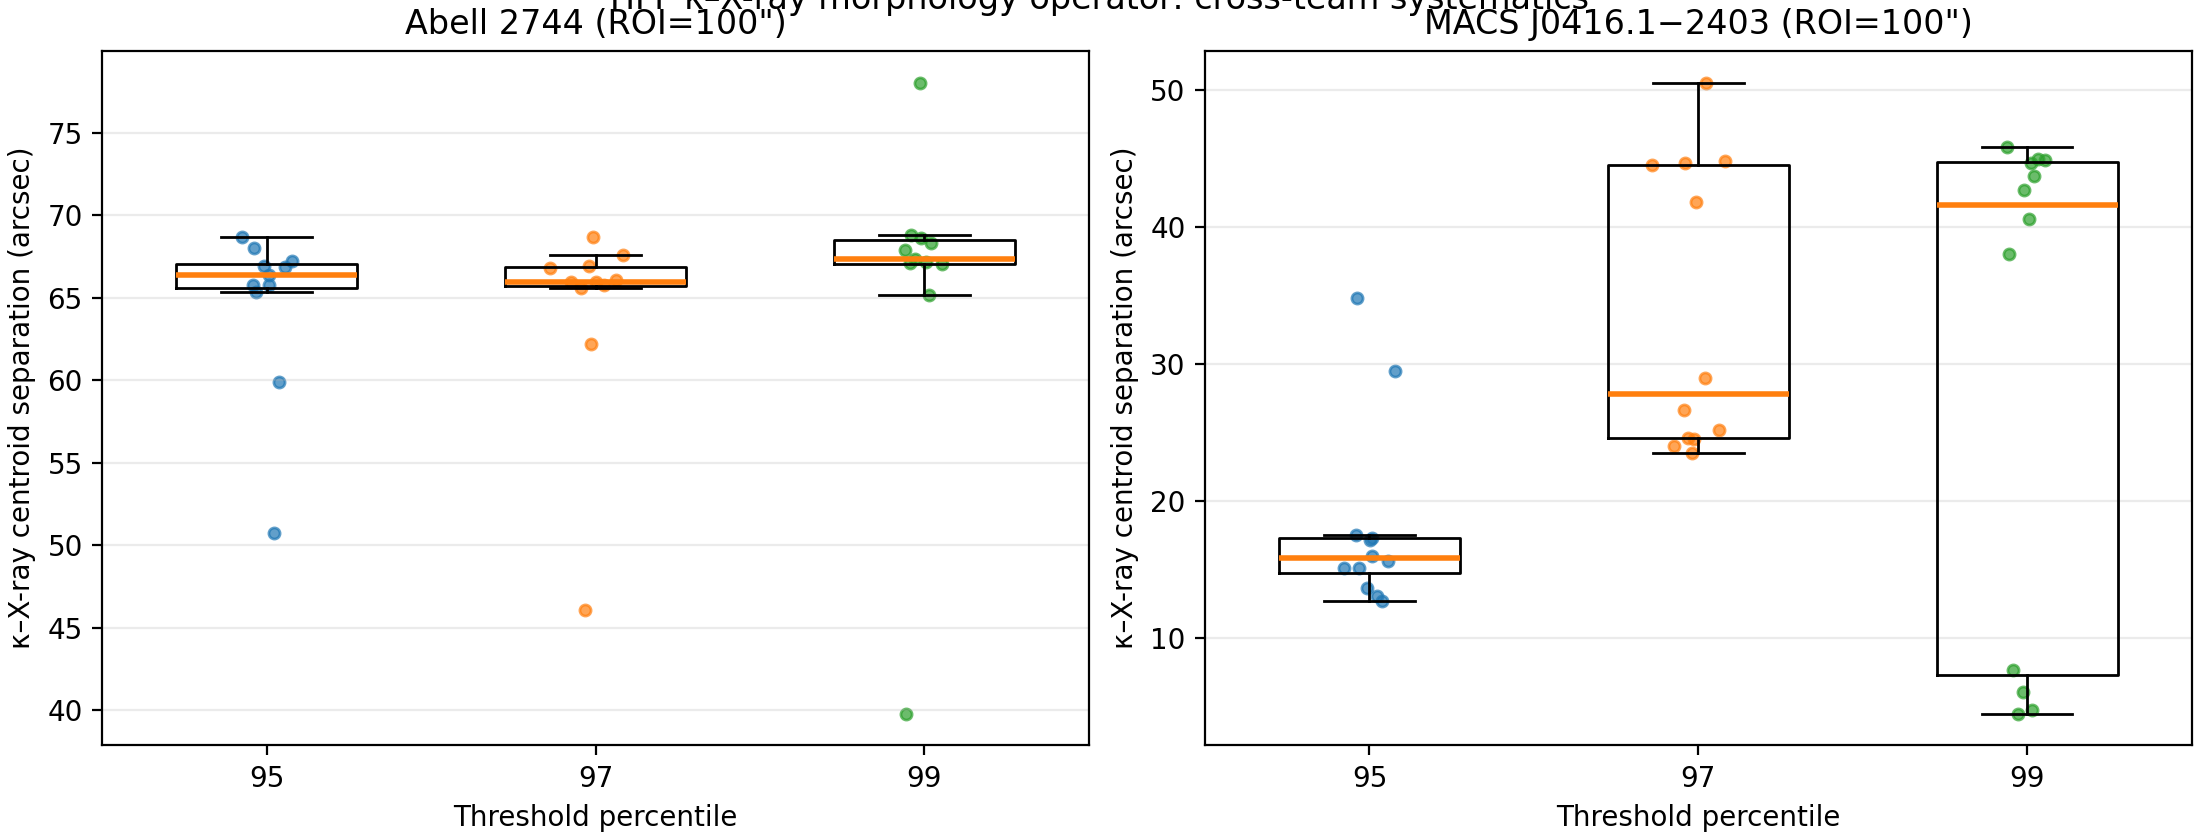
\includegraphics[width=6.5in,height=2.48182in]{media/image6.png}
\caption{\protect\phantomsection\label{_Toc222952642}{}Figure 6. HFF \(\kappa\)--X-ray systematics summary at ROI = 100″.}
\end{figure}

\subsection{C.4 Six-panel diagnostic figures (ROI = 100″)}\label{c.4-six-panel-diagnostic-figures-roi-100}

For interpretability, we generated per-team six-panel diagnostics at ROI = 100″, including κ, X-ray proxy, threshold masks, and centroid overlays. Representative examples are shown below; the complete figure sets are available from the author upon request.

\begin{figure}
\centering
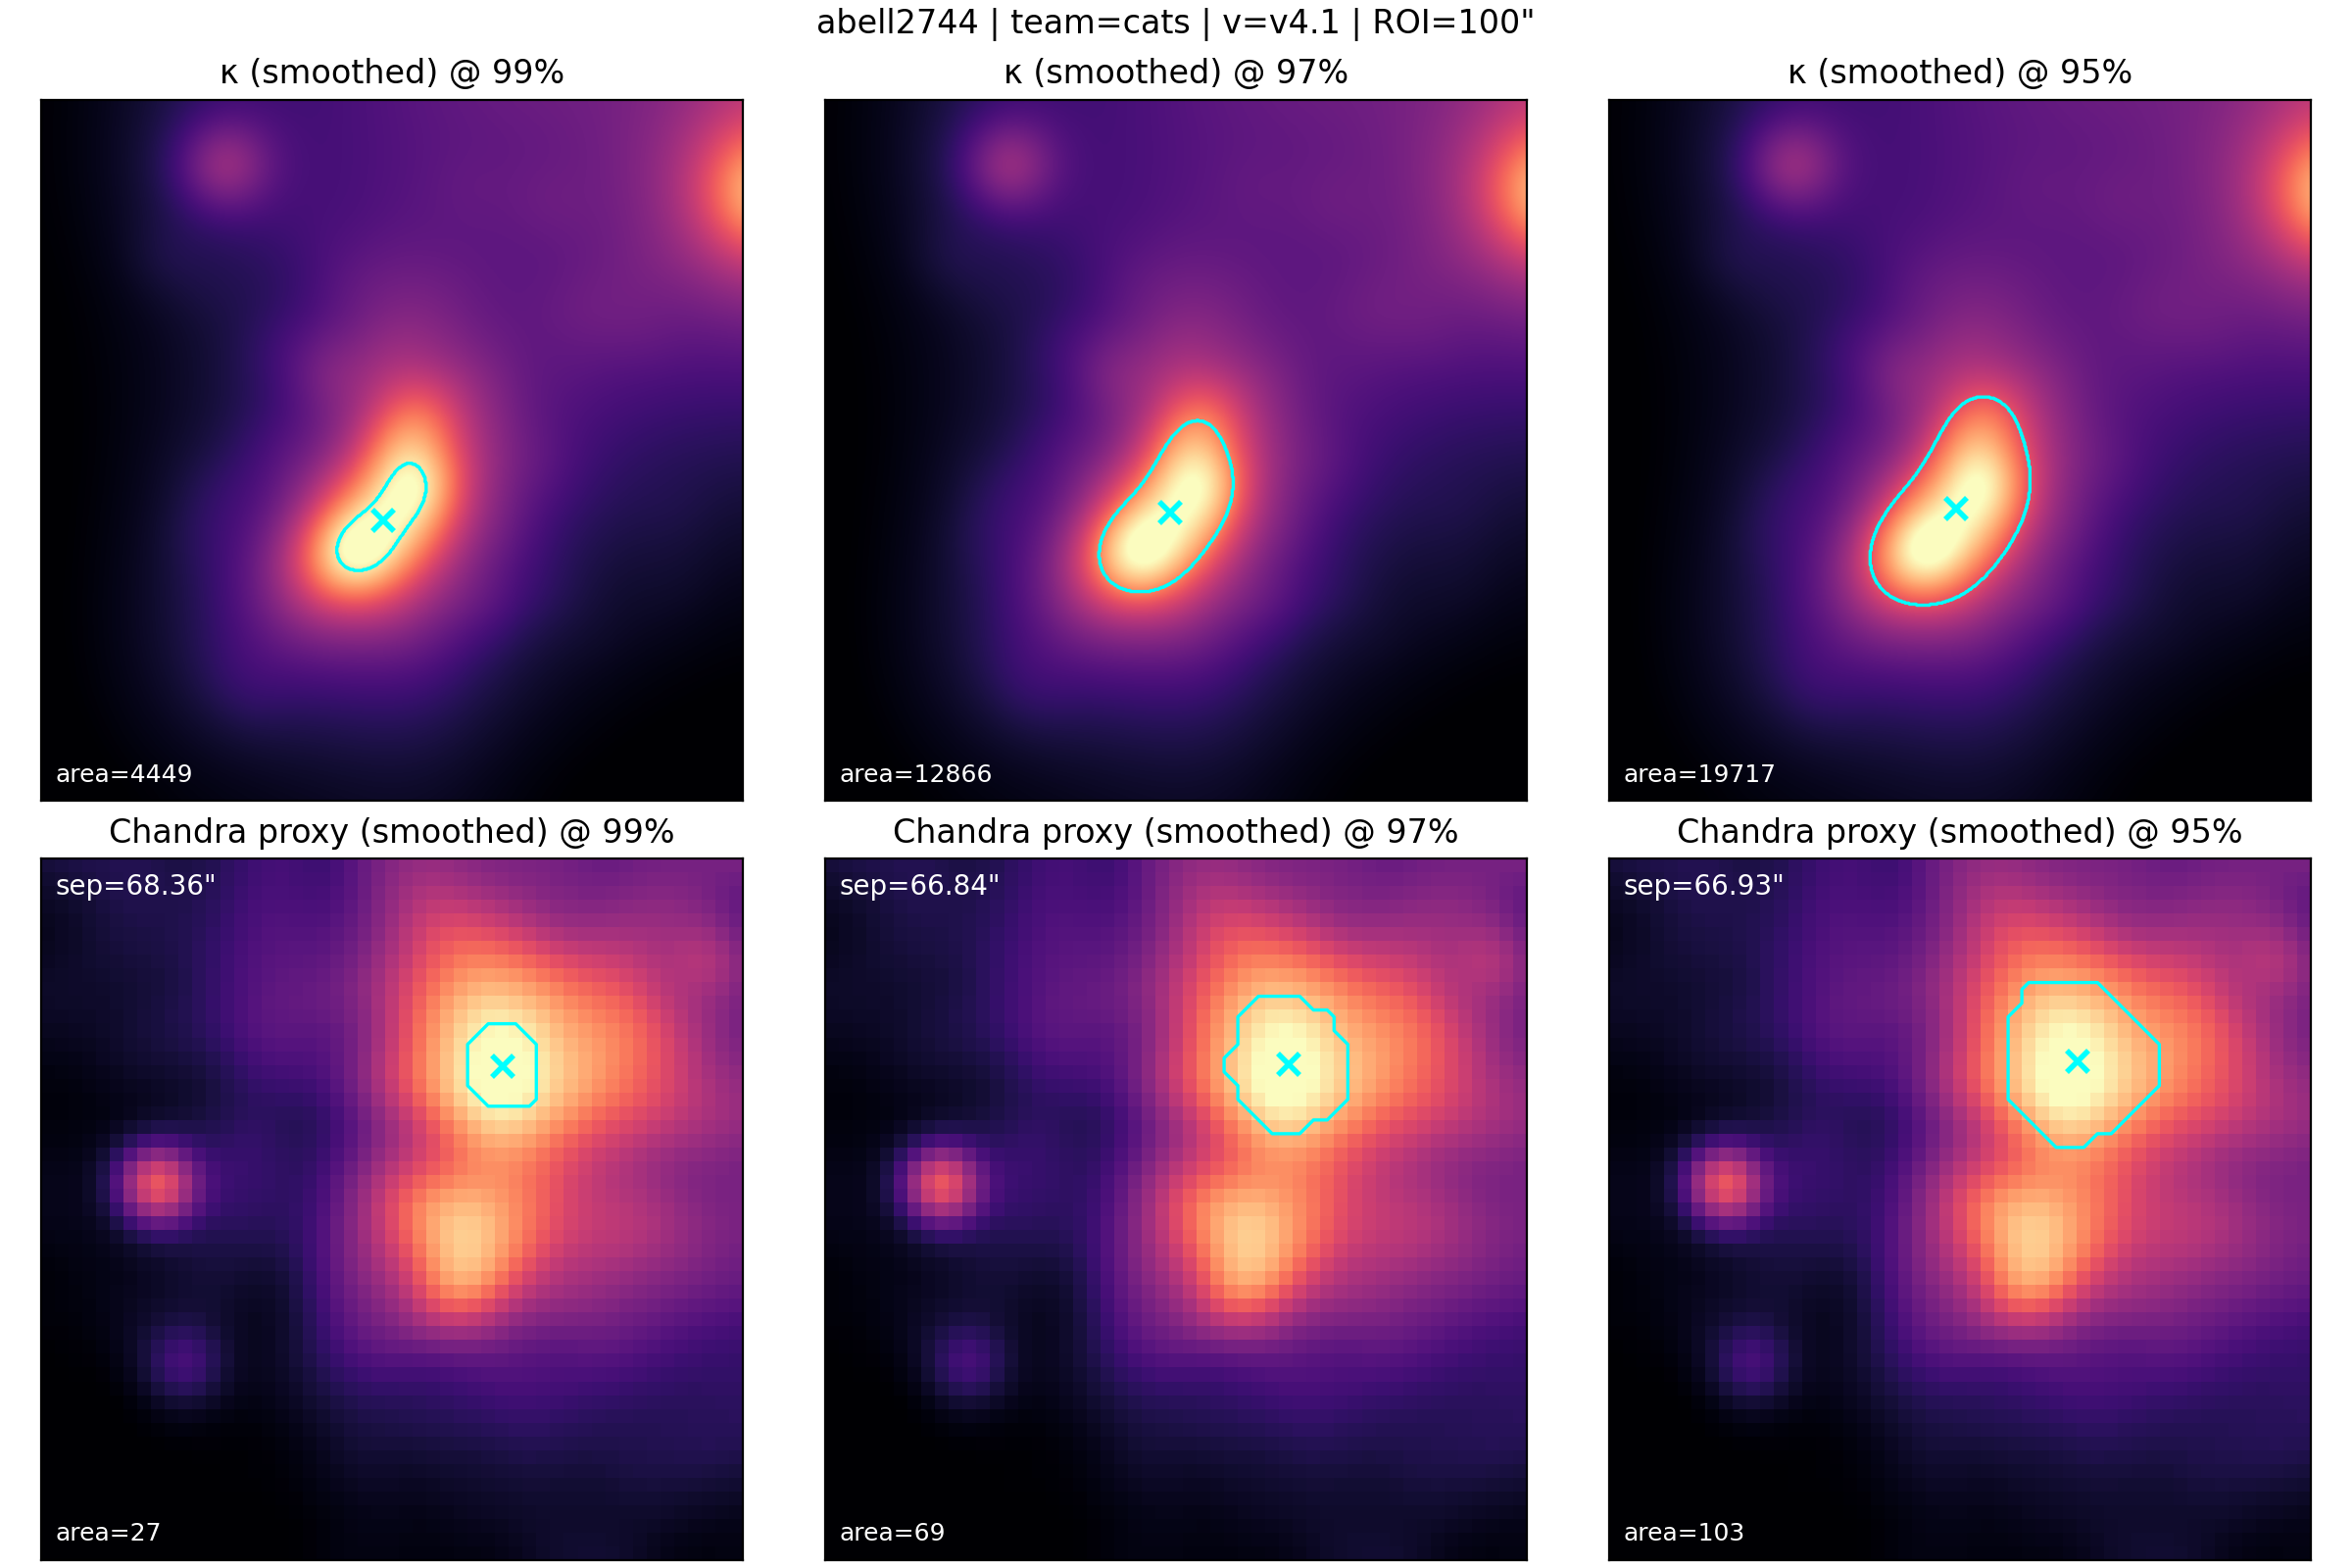
\includegraphics[width=6.5in,height=4.33333in]{media/image7.png}
\caption{\protect\phantomsection\label{_Toc222952643}{}Figure 7. Abell 2744 (CATS v4.1), ROI = 100″}
\end{figure}

\begin{figure}
\centering
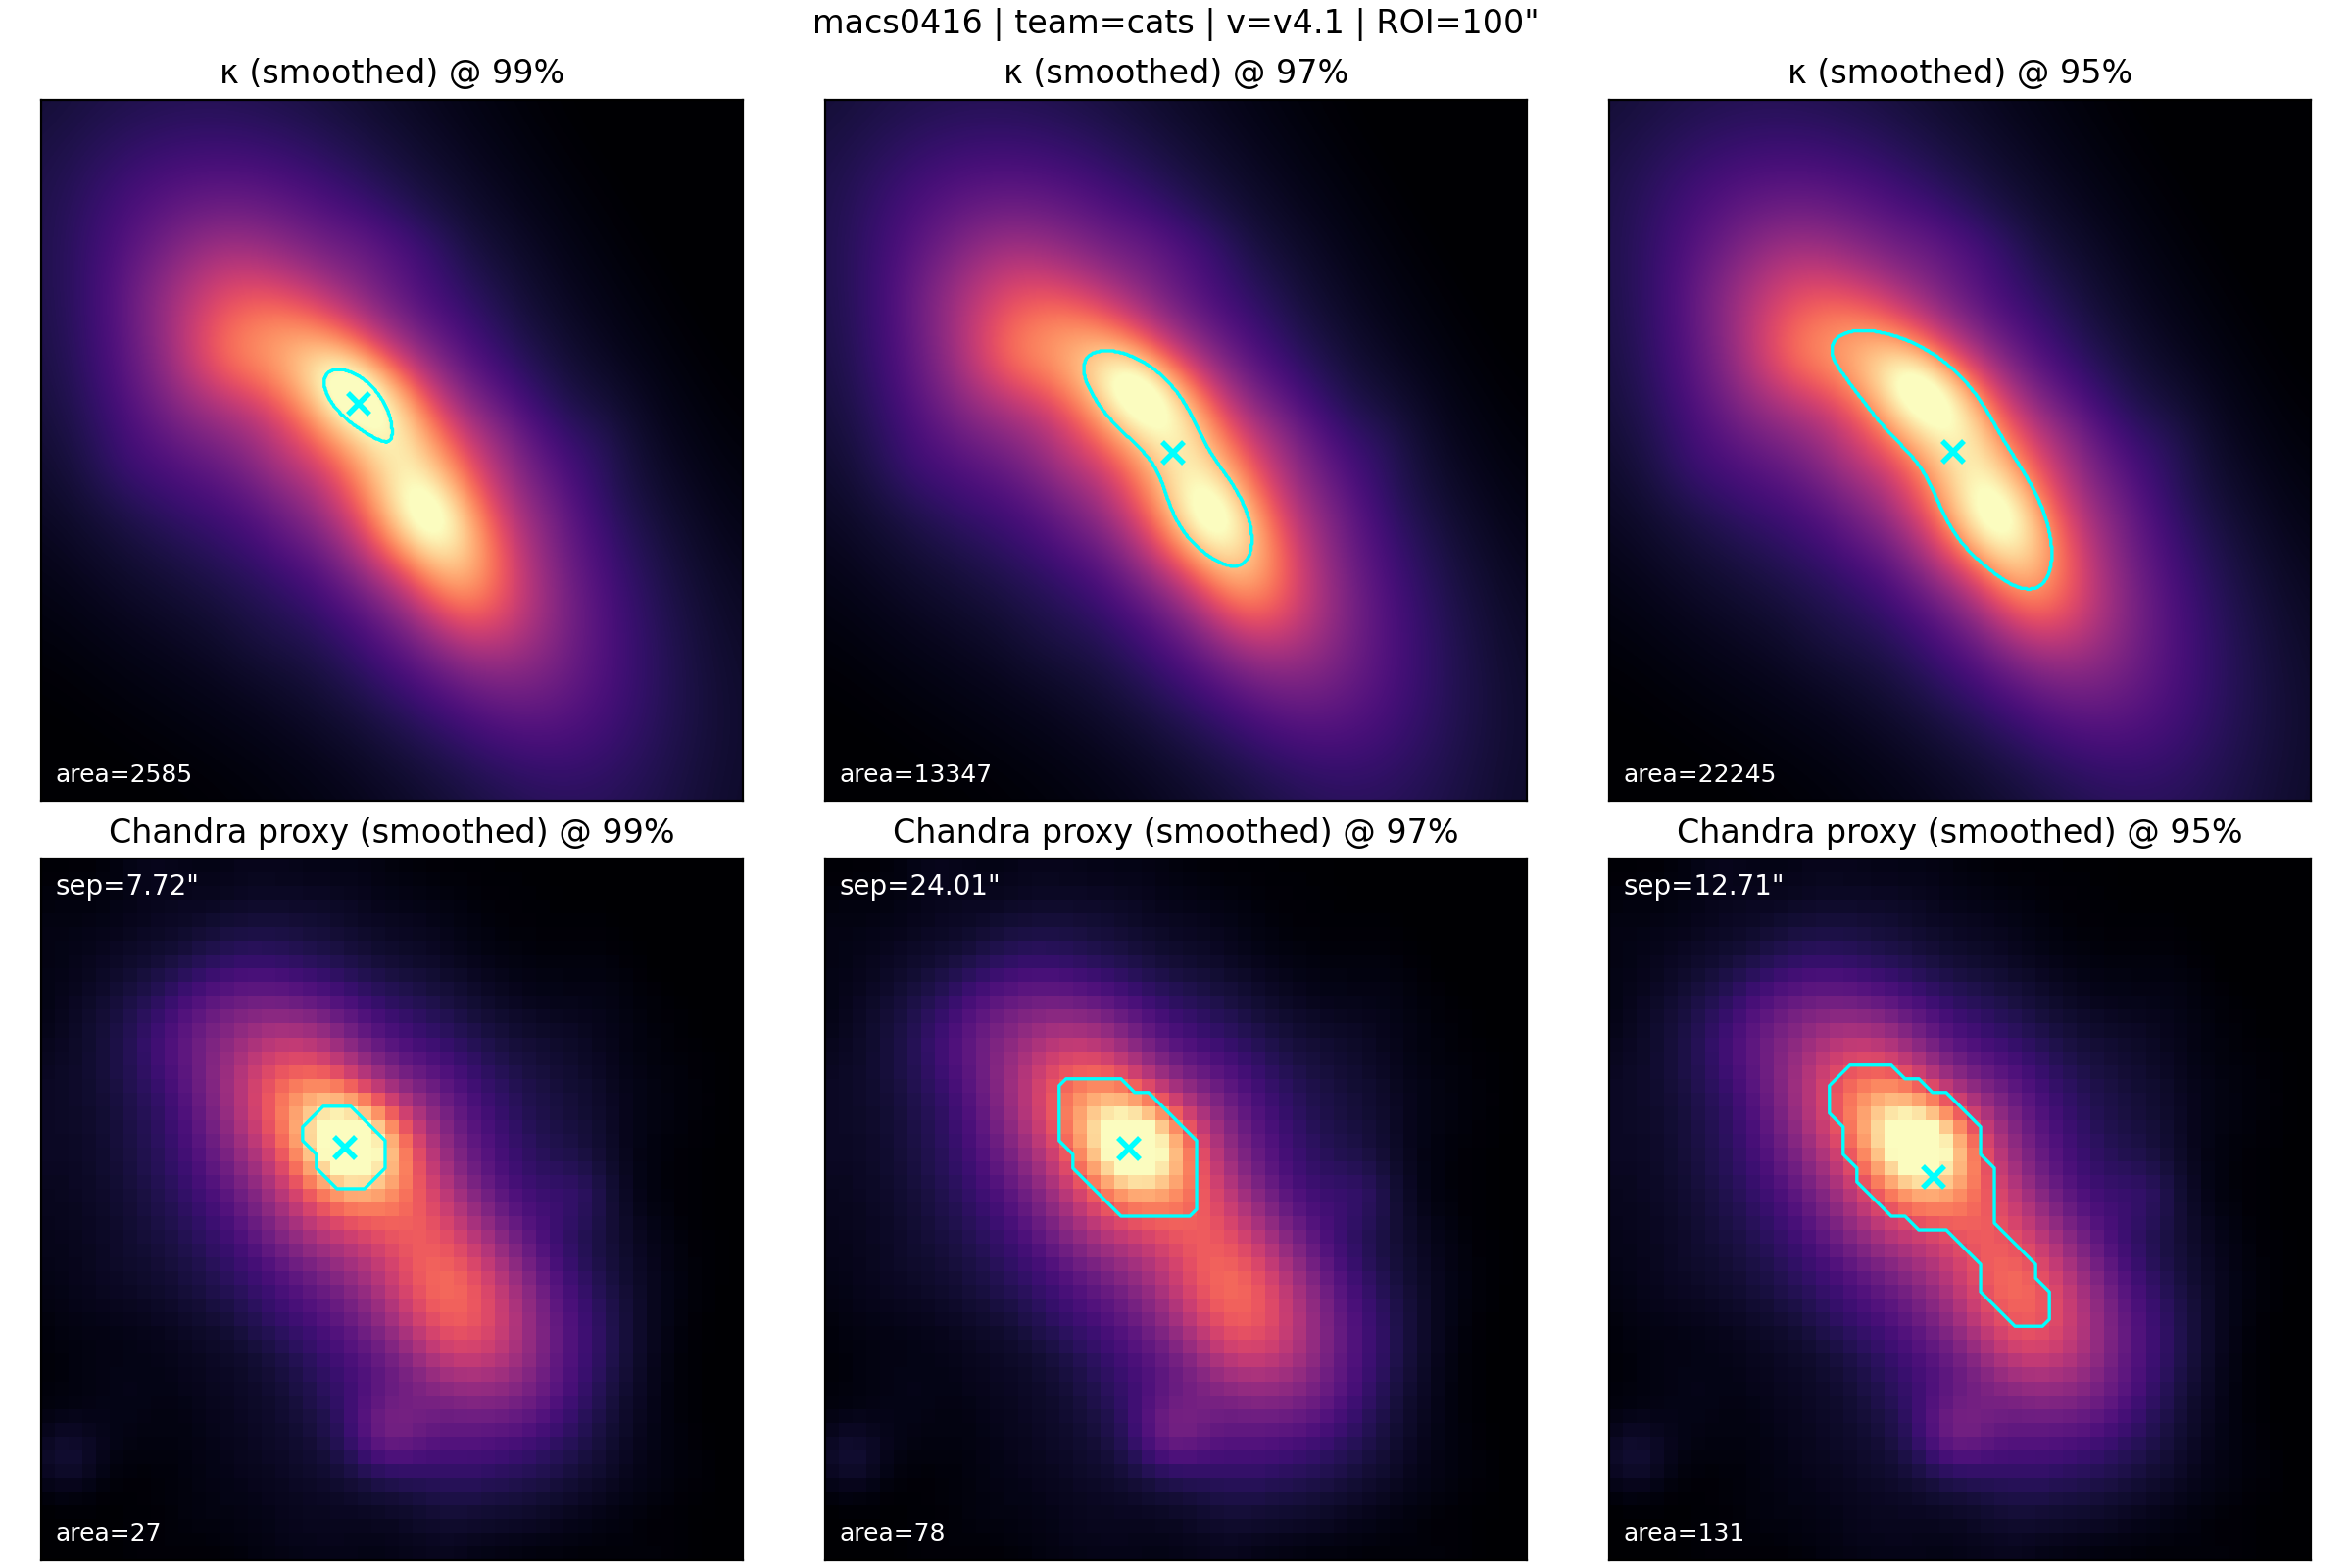
\includegraphics[width=6.5in,height=4.33333in]{media/image8.png}
\caption{\protect\phantomsection\label{_Toc222952644}{}Figure 8. MACS J0416.1−2403 (CATS v4.1), ROI = 100″.}
\end{figure}

\section{Appendix D. Spectral Harmonics and the Cymatic Analogy in Intrinsic Response Theory}\label{appendix-d.-spectral-harmonics-and-the-cymatic-analogy-in-intrinsic-response-theory}

\subsection{Purpose and scope}\label{d.1-purpose-and-scope}

This appendix formalizes the ``cymatics'' analogy used throughout the paper by identifying a single spectral object---the eigen-spectrum of an intrinsic response operator---that plays the same mathematical role as the Laplacian/biharmonic eigenmodes in Chladni plate experiments \citep{Rossing1982Chladni, Tuan2014Nodal} (Rossing, 1982). In brief: eigenfunctions are the response-sector mode shapes, eigenvalues set the characteristic spatial scales, and nodal sets correspond to compression/rarefaction boundaries. Although the underlying response dynamics may be written covariantly on spacetime (Carroll, 2019; Wald, 1984), the galaxy-rotation regime probed by SPARC is effectively stationary, so the empirically constrained ``harmonics'' are spatial overtones (additional radial nodes) rather than temporal frequency multiples.

\subsection{Unified operator statement (``DNA'' of intrinsic response)}\label{d.2-unified-operator-statement-dna-of-intrinsic-response}

Let \(\Phi_{resp}\) denote the response-sector potential (or any equivalent scalar response field used to encode the inferred metric perturbation in the weak-field limit). Define the intrinsic response through a driven, self-adjoint elliptic operator on a spatial slice:

\[\ \ \ \ \mathcal{L}\ \Phi_{resp} = \ S\left\lbrack \rho_{bar} \right\rbrack,\]

where \(S\left\lbrack \rho_{bar} \right\rbrack\) is the constitutive driving functional built from the baryonic sector, and the operator is taken in the minimal Sturm--Liouville form derived from \citep{BenderOrszag1999, KevorkianCole1996}

\[\ \ \ \ \mathcal{L}\  \equiv \  - \nabla \cdot \left( \alpha(x)\nabla\  \right) + \ \beta(x),\]

with \(\alpha(x) \geq \ 0\) controlling propagation (``permittivity/elasticity'') and β(x) ≥ 0 encoding activation/screening (``mass'' or quenching). The intrinsic ``pattern DNA'' is the eigen-spectrum

\[\ \ \ \ \mathcal{L}\ \varphi_{n} = \ \lambda_{n}\varphi_{n},\ \ \ \left\langle \varphi_{m},\ \varphi_{n} \right\rangle = \ \delta_{mn},\]

yielding the modal response

\[\ \ \ \ \Phi_{resp(x)} = \ \Sigma_{n}c_{n}\varphi_{n(x)},\ \ \ c_{n} = \frac{\left\langle \varphi_{n},\ S \right\rangle}{\lambda_{n}}.\]

This is a direct analog of Chladni/cymatics: \(\varphi_{n}\) are mode shapes; the \(\lambda_{n}\) set intrinsic spatial scales; and the source overlap \(\left\langle \varphi_{n},\ S \right\rangle\) is the excitation/selection rule that determines which modes are visible in a given galaxy.

\subsection{Where ``harmonics'' live in a unified spacetime theory}\label{d.3-where-harmonics-live-in-a-unified-spacetime-theory}

In the covariant formulation \citep{HawkingEllis1973, Wald1984GR, Carroll2019Spacetime}, Spacetime unification means that the fundamental response dynamics can be written covariantly (e.g., for a scalar template, a hyperbolic operator \(\mathcal{D}\) such as (□ \(–\ m\_ eff\hat{}2)\chi\  = \ J\)). In stationary or quasi-stationary systems, variable separation reduces the covariant problem to a spatial eigenproblem: \(\chi(t,\ x) = \ \Sigma_{n}q_{n(t)\varphi_{n(x)}}\), where \(\varphi_{n}\) are eigenfunctions of the induced spatial operator \(\mathcal{L}\) and \(q_{n}(t)\) obey driven oscillator equations with characteristic frequencies \(\Omega_{n}^{2} \propto \ \lambda_{n}\). SPARC rotation curves constrain the near-static regime in which \(q_{n}(t)\) has equilibrated, leaving the spatial spectral content as the observable imprint (Carroll, 2019; Hawking \& Ellis, 1973; Wald, 1984).

\subsection{Observable proxy: node count and Δ-sign flips in the SPARC window}\label{d.4-observable-proxy-node-count-and-ux3b4-sign-flips-in-the-sparc-window}

SPARC provides baryonic mass models and high-quality rotation curves for 175 disk galaxies (Lelli et al., 2016). Define \(\Delta(R)\) operationally \citep{McGaughSchombert2014ML, Ivezic2019LSST} as the signed residual between the observed and baryonic expectations in the rotation curve (e.g., \(\Delta v^{2(R)} \equiv \ v_{obs}^{2}–\ v_{bar}^{2}\)). In an oscillatory response sector, \(\Phi_{resp}\) (and therefore the inferred extra acceleration) can alternate in sign across radius, producing compression and rarefaction lobes. In the operator language above, each change in radial sign in \(\Delta(R)\) corresponds to crossing a nodal annulus/shell of the net excited response pattern \(\Sigma_{n}c_{n}\varphi_{n}\). Hence, within the finite SPARC radial sampling window, the number of \(\Delta\)-sign flips provides a model-agnostic proxy for the degree of higher-\(n\) (harmonic/overtone) participation: zero flips indicates a fundamental-dominated response; multiple flips indicate increasing harmonic content (higher node count) selected by \(\left\langle \varphi_{n},\ S \right\rangle\) and by activation/quenching boundaries.

\subsection{Consequences for lensing and stability constraints}\label{d.5-consequences-for-lensing-and-stability-constraints}

Because the response tensor is effectively inferred from kinematics, sign-alternating lobes should be treated as an empirical prediction of the effective sector rather than as an immediate pathology. In particular, annular rarefaction phases imply a ring-like suppression of weak-lensing observables (e.g., \(\Delta\Sigma\) or \(\kappa\) relative to control stacks) in the same radial ranges, providing a falsifiable discriminant using upcoming wide-field surveys (Scaramella et al., 2022; Euclid Collaboration, 2025; Ivezić et al., 2019). At the fundamental level, \citep{BuniyHsuMurray2006NEC, Rubakov2006NEC, Rubakov2014NECReview} the minimal non-negotiable stability line is to keep the underlying response-field EFT free of ghosts/gradient instabilities; for broad k-essence classes this is ensured by requiring a positive kinetic coefficient (\(P_{,X} \geq \ 0\)), which enforces the null energy condition for the fundamental field stress-energy even if the effective, inverse-constructed response density changes sign locally (Rubakov, 2006). For context, relativistic MOND completions (e.g., TeVeS) also introduce extra fields that alter lensing but do not generically predict phase-correlated annular suppression tied to \(\Delta\)-sign flips (Bekenstein, 2004).

\section{References}\label{}

% BibTeX bibliography (see references.bib)
% APA 7th bibliography style with author-date format
% Include ALL entries from references.bib (not just cited ones)
\nocite{*}
\bibliographystyle{apalike}
\bibliography{references}

\iffalse % legacy manual bibliography (disabled)

Ackermann, M., et al. (2015). Searching for dark matter annihilation from Milky Way dwarf spheroidal galaxies. Physical Review Letters, 115(23), 231301. https://doi.org/10.1103/PhysRevLett.115.231301

Aguilar, M., et al. (2013). First result from the Alpha Magnetic Spectrometer on the International Space Station. Physical Review Letters, 110(14), 141102. https://doi.org/10.1103/PhysRevLett.110.141102

Akerib, D. S., et al. (2017). Results from a search for dark matter in the complete LUX exposure. Physical Review Letters, 118(2), 021303. https://doi.org/10.1103/PhysRevLett.118.021303

Aprile, E., et al. (2018). Dark matter search results from a one-ton-year exposure of XENON1T. Physical Review Letters, 121(11), 111302. https://doi.org/10.1103/PhysRevLett.121.111302

Bekenstein, J. D. (2004). Relativistic gravitation theory for the modified Newtonian dynamics paradigm. Physical Review D, 70(8), 083509. https://doi.org/10.1103/PhysRevD.70.083509

Bender, C. M., \& Orszag, S. A. (1999). Advanced Mathematical Methods for Scientists and Engineers I. Springer. https://doi.org/10.1007/978-1-4757-3069-2

Bosma, A. (1978). The distribution and kinematics of neutral hydrogen in spiral galaxies of type Sab--Scd. PhD Thesis, University of Groningen.

Buchert, T. (2000). On average properties of inhomogeneous fluids in general relativity: Dust cosmologies. General Relativity and Gravitation, 32(1), 105--125. https://doi.org/10.1023/A:1001800617177

Buniy, R. V., Hsu, S. D. H., \& Murray, B. M. (2006). The null energy condition and instability. Physical Review D, 74, 063518. https://doi.org/10.1103/PhysRevD.74.063518

Burgess, C. P. (2004). Quantum gravity in everyday life: General relativity as an effective field theory. Living Reviews in Relativity, 7(1), 5. https://doi.org/10.12942/lrr-2004-5

Carroll, S. M. (2004). Spacetime and Geometry: An Introduction to General Relativity. Addison-Wesley.

Carroll, S. M. (2019). Spacetime and geometry: An introduction to general relativity. Cambridge University Press. https://doi.org/10.1017/9781108770385

Clowe, D., et al. (2006). A direct empirical proof of the existence of dark matter. Astrophysical Journal Letters, 648(2), L109--L113. https://doi.org/10.1086/508162

Cui, X., et al. (2017). Dark matter results from 54-ton-day exposure of PandaX-II experiment. Physical Review Letters, 119(18), 181302. https://doi.org/10.1103/PhysRevLett.119.181302

Deser, S., \& Woodard, R. P. (2007). Nonlocal cosmology. Physical Review Letters, 99(11), 111301. https://doi.org/10.1103/PhysRevLett.99.111301

Donoghue, J. F. (1994). General relativity as an effective field theory: The leading quantum corrections. Physical Review D, 50(6), 3874--3888. https://doi.org/10.1103/PhysRevD.50.3874

Einstein, A. (1915). Erklärung der Perihelbewegung des Merkur aus der allgemeinen Relativitätstheorie. Sitzungsberichte der Königlich Preußischen Akademie der Wissenschaften, 831--839.

Einstein, A. (1916). Die Grundlage der allgemeinen Relativitätstheorie. Annalen der Physik, 354(7), 769--822.

Euclid Collaboration. (2022). Euclid preparation. I. The Euclid Wide Survey. Astronomy \& Astrophysics, 662, A112. https://doi.org/10.1051/0004-6361/202141938

Euclid Collaboration. (2025). Euclid. I. Overview of the Euclid mission. Astronomy \& Astrophysics, 697, A1. https://doi.org/10.1051/0004-6361/202450810

Fruscione, A., et al. (2006). CIAO: Chandra's Data Analysis System. Proceedings of SPIE, 6270, 62701V. https://cxc.cfa.harvard.edu/ciao/

Hawking, S. W., \& Ellis, G. F. R. (1973). The large scale structure of space-time. Cambridge University Press. https://doi.org/10.1017/CBO9780511524646

Ivezić, Ž., Kahn, S. M., Tyson, J. A., Abel, B., Acosta, E., Allsman, R., Alonso, D., AlSayyad, Y., Anderson, S. F., Andrew, J., Angel, J. R. P., Angeli, G. Z., Ansari, R., Antilogus, P., Araujo, C., Armstrong, R., Arndt, K. T., Astier, P., Aubourg, É., \ldots{} LSST Collaboration. (2019). LSST: From science drivers to reference design and anticipated data products. The Astrophysical Journal, 873(2), 111. https://doi.org/10.3847/1538-4357/ab042c

Kevorkian, J., \& Cole, J. D. (1996). Multiple Scale and Singular Perturbation Methods. Springer. https://doi.org/10.1007/978-1-4612-3968-4

Le Verrier, U. J. (1859). Théorie du mouvement de Mercure. Annales de l'Observatoire de Paris, 5, 1--196.

Lelli, F., McGaugh, S. S., \& Schombert, J. M. (2016). SPARC: Mass models for 175 disk galaxies with Spitzer photometry and accurate rotation curves. The Astronomical Journal, 152(6), 157. https://doi.org/10.3847/0004-6256/152/6/157

McGaugh, S. S., \& Schombert, J. M. (2014). Color--mass-to-light-ratio relations for disk galaxies. The Astronomical Journal, 148(5), 77. https://doi.org/10.1088/0004-6256/148/5/77

McGaugh, S. S., Schombert, J. M., Bothun, G. D., \& de Blok, W. J. G. (2000). The baryonic Tully--Fisher relation. The Astrophysical Journal, 533(2), L99--L102. https://doi.org/10.1086/312628

Mikulski Archive for Space Telescopes (MAST). (2019). Hubble Space Telescope Frontier Fields (HLSP archive). Retrieved February 24, 2026, from https://archive.stsci.edu/hlsp/frontier/

Milgrom, M. (1983). A modification of the Newtonian dynamics as a possible alternative to the hidden mass hypothesis. The Astrophysical Journal, 270, 365--370. https://doi.org/10.1086/161130

NASA/GSFC HEASARC. (2025). Archive access and documentation. Retrieved February 24, 2026, from https://heasarc.gsfc.nasa.gov/docs/archive.html

Planck Collaboration. (2020). Planck 2018 results. VI. Cosmological parameters. Astronomy \& Astrophysics, 641, A6. https://doi.org/10.1051/0004-6361/201833910

Poisson, E., \& Will, C. M. (2014). Gravity: Newtonian, Post-Newtonian, Relativistic. Cambridge University Press.

Räsänen, S. (2006). Accelerated expansion from structure formation. Journal of Cosmology and Astroparticle Physics, 2006(11), 003. https://doi.org/10.1088/1475-7516/2006/11/003

Riess, A. G., et al. (2019). Large Magellanic Cloud Cepheid standards provide a 1\% foundation for the determination of the Hubble constant. The Astrophysical Journal, 876(1), 85. https://doi.org/10.3847/1538-4357/ab1422

Rossing, T. D. (1982). Chladni's law for vibrating plates. American Journal of Physics, 50(3), 271--274. https://doi.org/10.1119/1.12866

Rubakov, V. A. (2006). The null energy condition and instability. Physical Review D, 74(6), 063518. https://doi.org/10.1103/PhysRevD.74.063518

Rubakov, V. A. (2014). The null energy condition and its violation. Physics-Uspekhi, 57(2), 128--142. https://doi.org/10.3367/UFNE.0184.201402B.0137

Rubin, V. C., \& Ford, W. K. (1970). Rotation of the Andromeda Nebula from a spectroscopic survey of emission regions. The Astrophysical Journal, 159, 379. https://doi.org/10.1086/150317

Scaramella, R., Amiaux, J., Mellier, Y., Burigana, C., Carvalho, C. S., Cuillandre, J.-C., \ldots{} Euclid Collaboration. (2022). Euclid preparation. I. The Euclid Wide Survey. Astronomy \& Astrophysics, 662, A112. https://doi.org/10.1051/0004-6361/202141938

Tuan, P. H., Bambi, C., Giannoni, M.-J., \& Li, J.-J. (2014). From vibrating plates to laser cavities: Nodal patterns and semiclassical correspondence. Physical Review E, 89(2), 022911. https://doi.org/10.1103/PhysRevE.89.022911

Verlinde, E. (2017). Emergent gravity and the dark universe. SciPost Physics, 2, 016. https://doi.org/10.21468/SciPostPhys.2.3.016

Wald, R. M. (1984). General relativity. University of Chicago Press. https://doi.org/10.7208/chicago/9780226870373.001.0001
\fi
\end{document}
